% !TEX program = xelatex
\documentclass[8pt,aspectratio=169]{beamer}
\usetheme[numbering=none,block=fill]{metropolis}
\usepackage[backend=bibtex,url=false,doi=false,maxcitenames=1, style=authoryear]{biblatex}
\usepackage{amsthm,amsmath,amssymb,braket,fontspec,unicode-math,appendixnumberbeamer,pifont}
\usepackage[absolute,overlay]{textpos}

\setbeamertemplate{frametitle continuation}{}
\setbeamerfont{alerted text}{series=\bfseries}

\makeatletter
\def\@makefnmark{}
\makeatletter

\makeatletter
\setlength{\metropolis@titleseparator@linewidth}{2pt}
\setlength{\metropolis@progressonsectionpage@linewidth}{2pt}
\setlength{\metropolis@progressinheadfoot@linewidth}{2pt}
\makeatother



\setbeamertemplate{footline}{%
  \begin{beamercolorbox}[wd=\textwidth, sep=1ex]{footline}%
    \hspace{0.3cm}
    \usebeamerfont{page number in head/foot}%
    \usebeamertemplate*{frame footer}
    \hfill%
    \usebeamertemplate*{frame numbering}
  \end{beamercolorbox}%
}


\setbeamertemplate{section page}{
  \begin{minipage}{\linewidth}
  \centering
  \raggedright
  \usebeamercolor[fg]{section title}
  \usebeamerfont{section title}
  {\huge \insertsectionhead}\\[-1ex]
  \usebeamertemplate*{progress bar in section page}
  \par
  \ifx\insertsubsectionhead\@empty\else%
    \usebeamercolor[fg]{subsection title}%
    \usebeamerfont{subsection title}%
    \insertsubsectionhead
  \fi
  \end{minipage}
  \par
  \vspace{\baselineskip}
}


\setmainfont{Fira Sans}
\setsansfont{Fira Sans}
\setmathfont{Fira Math}
\setmathfont{Latin Modern Math}[range={frak,\bigcap,\bigcup}]


\setbeamercolor{footnote}{fg=navyblue}
\setbeamerfont{footnote}{series=\bfseries}
\setbeamerfont{title}{size=\huge,shape=\scshape}

\bibliography{bib}
\AtBeginBibliography{\scriptsize}

\newcommand{\focus}[1]{\textcolor{red}{\bf{#1}}}
\newcommand{\nitem}{\item[\ding{51}]}

\definecolor{red}{HTML}{CC0000}
\definecolor{lred}{HTML}{e24a33}
\definecolor{lblue}{HTML}{348abd}
\definecolor{navyblue}{HTML}{000080}
\setbeamertemplate{bibliography item}[triangle]

\graphicspath{{./figures/}} % Change the path

\setbeamerfont{institute}{size=\large}
\setbeamerfont{author}{size=\large}
\setbeamerfont{date}{size=\large}

\title{\vspace*{\fill}Emergence in free and correlated fermions: from impurity models to the bulk}
\subtitle{JRF-to-SRF Upgradation Presentation}
\author{
{\bf Abhirup Mukherjee}}

\date{\today \hspace*{0.25\textwidth} Supervisor: Dr. Siddhartha Lal}

\institute{Department of Physical Sciences, IISER Kolkata, Mohanpur\\[20pt]

\includegraphics[width=0.1\textwidth]{figures/epqm_logo_mod.jpeg}
\hspace*{\fill}

\includegraphics[width=0.1\textwidth]{figures/dps_logo.jpeg}
\hspace*{\fill}

\includegraphics[width=0.1\textwidth]{figures/IISER-K_Logo.png}
\vspace*{-20pt}
}

\begin{document}

\centering

\begin{frame}
\maketitle
% \begin{textblock*}{\textwidth}(0.5cm, 7.3cm)
% 	\centering
% 	
\includegraphics[width=0.1\textwidth]{figures/epqm_logo_mod.jpeg}
% 	\hspace*{\fill}
% 	
\includegraphics[width=0.1\textwidth]{figures/dps_logo.jpeg}
% 	\hspace*{\fill}
% 	
\includegraphics[width=0.1\textwidth]{figures/IISER-K_Logo.png}
% \end{textblock*}
\end{frame}

\begin{frame}{}
% \flushleft
% 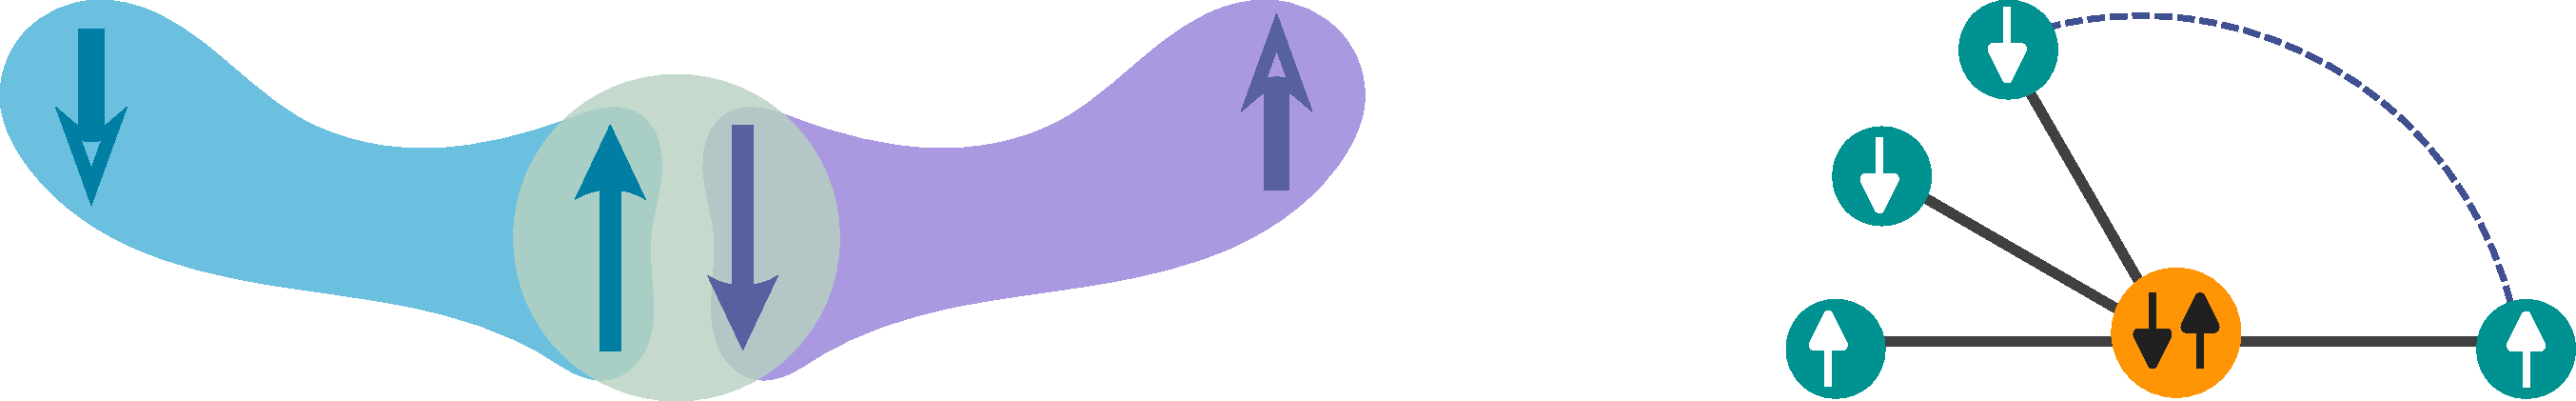
\includegraphics[width=0.6\textwidth]{./figures/summary.pdf}

% \vspace*{40pt}

\section{Summary of Work}

% \vspace*{30pt}

% \flushright
% 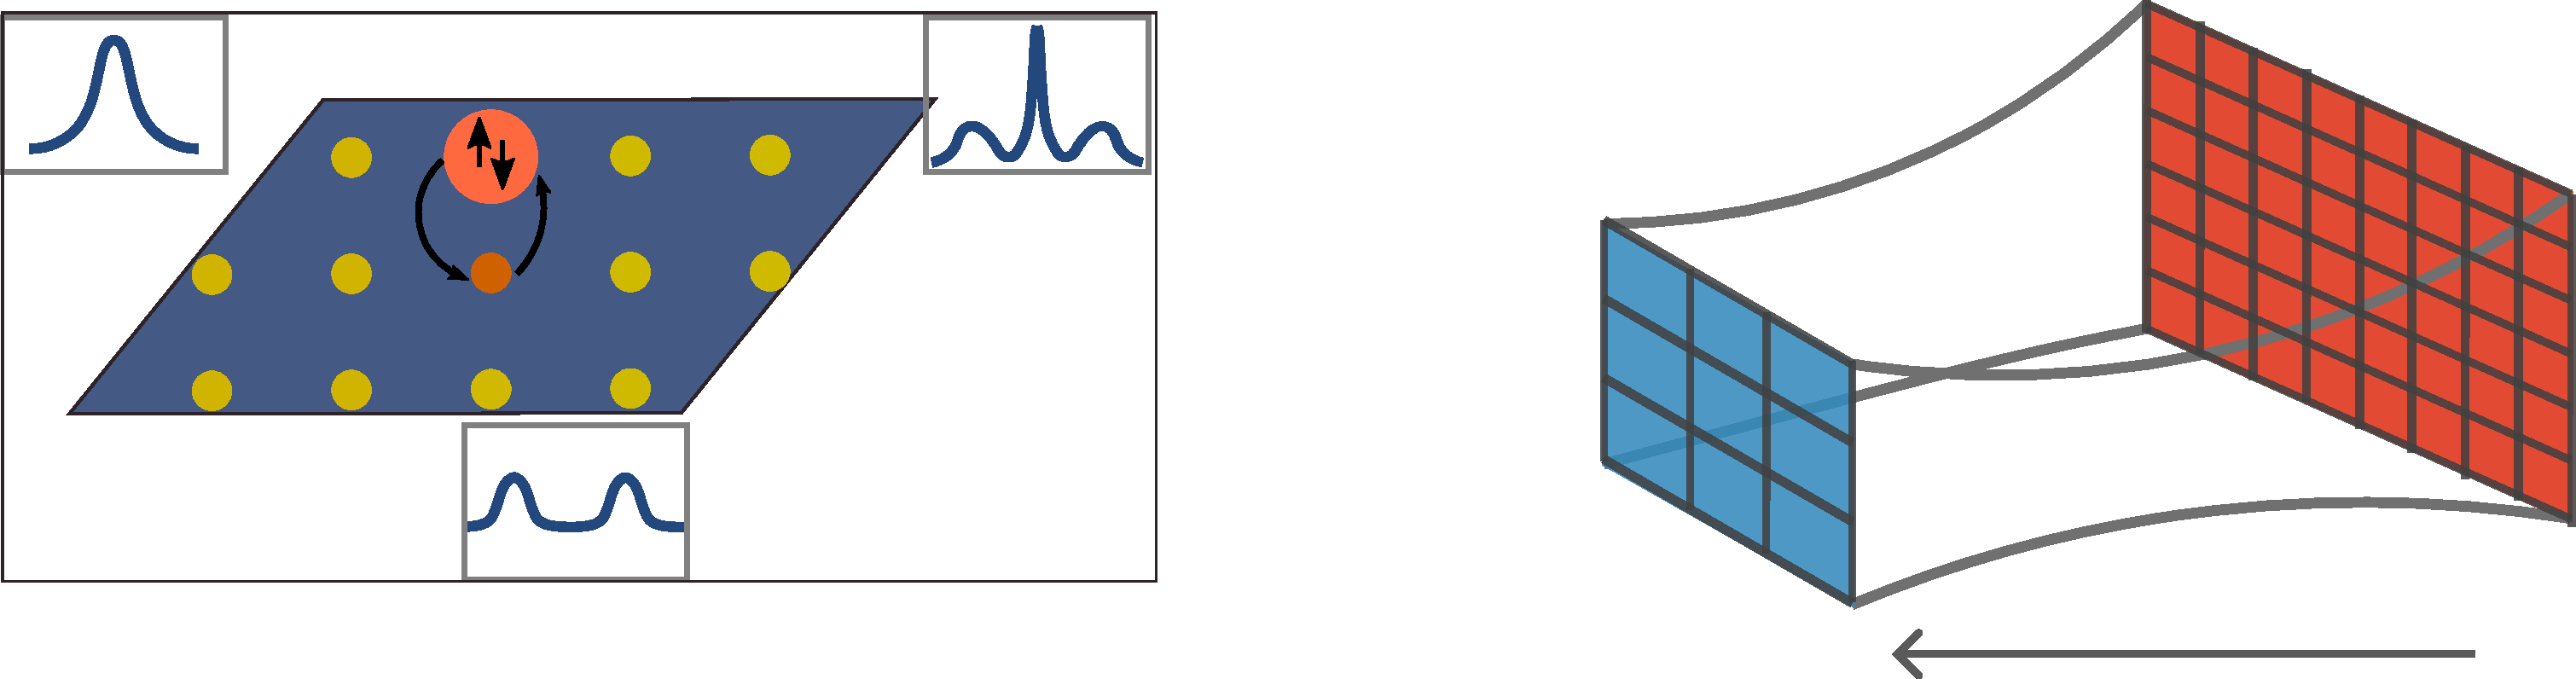
\includegraphics[width=0.6\textwidth]{./figures/summary2.pdf}
\end{frame}

\begin{frame}{Summary of Work}
\flushleft 
{\bf Completed Projects}
\vspace*{\fill}
\begin{itemize}
\nitem Unveiling the Kondo cloud: Unitary renormalization-group study of the Kondo model \\[2pt]
{\small\alert{Phys. Rev. B 105, 085119}, arXiv:2111.10580v3}\\
{\small A. Mukherjee, {\it Abhirup Mukherjee}, N. S. Vidhyadhiraja, A. Taraphder, and S. Lal}\\[10pt]

\nitem Frustration shapes multi-channel Kondo physics: A star graph perspective\\[2pt]
\small{\alert{under review at PRB}, arXiv:2205.00790\\
S. Patra, {\it Abhirup Mukherjee}, A. Mukherjee, N. S. Vidhyadhiraja, A. Taraphder, S. Lal} \\[10pt]
\end{itemize}
\vspace*{\fill}

{\bf Ongoing Projects}
\vspace*{\fill}
\begin{itemize}
	\nitem \underline{Metal-insulator transition in an extended Anderson impurity model} ({\it \small{manuscript in preparation}})\\[10pt]
	\nitem Holography and topology of entanglement scaling in free fermions ({\it \small{manuscript in preparation}})\\[10pt]
	\nitem URG-based auxiliary model approach to correlated systems ({\it \small{ongoing}})
\end{itemize}

\end{frame}

\begin{frame}{}
\section{Local MIT in an extended Anderson impurity model}

\begin{minipage}{0.5\textwidth}
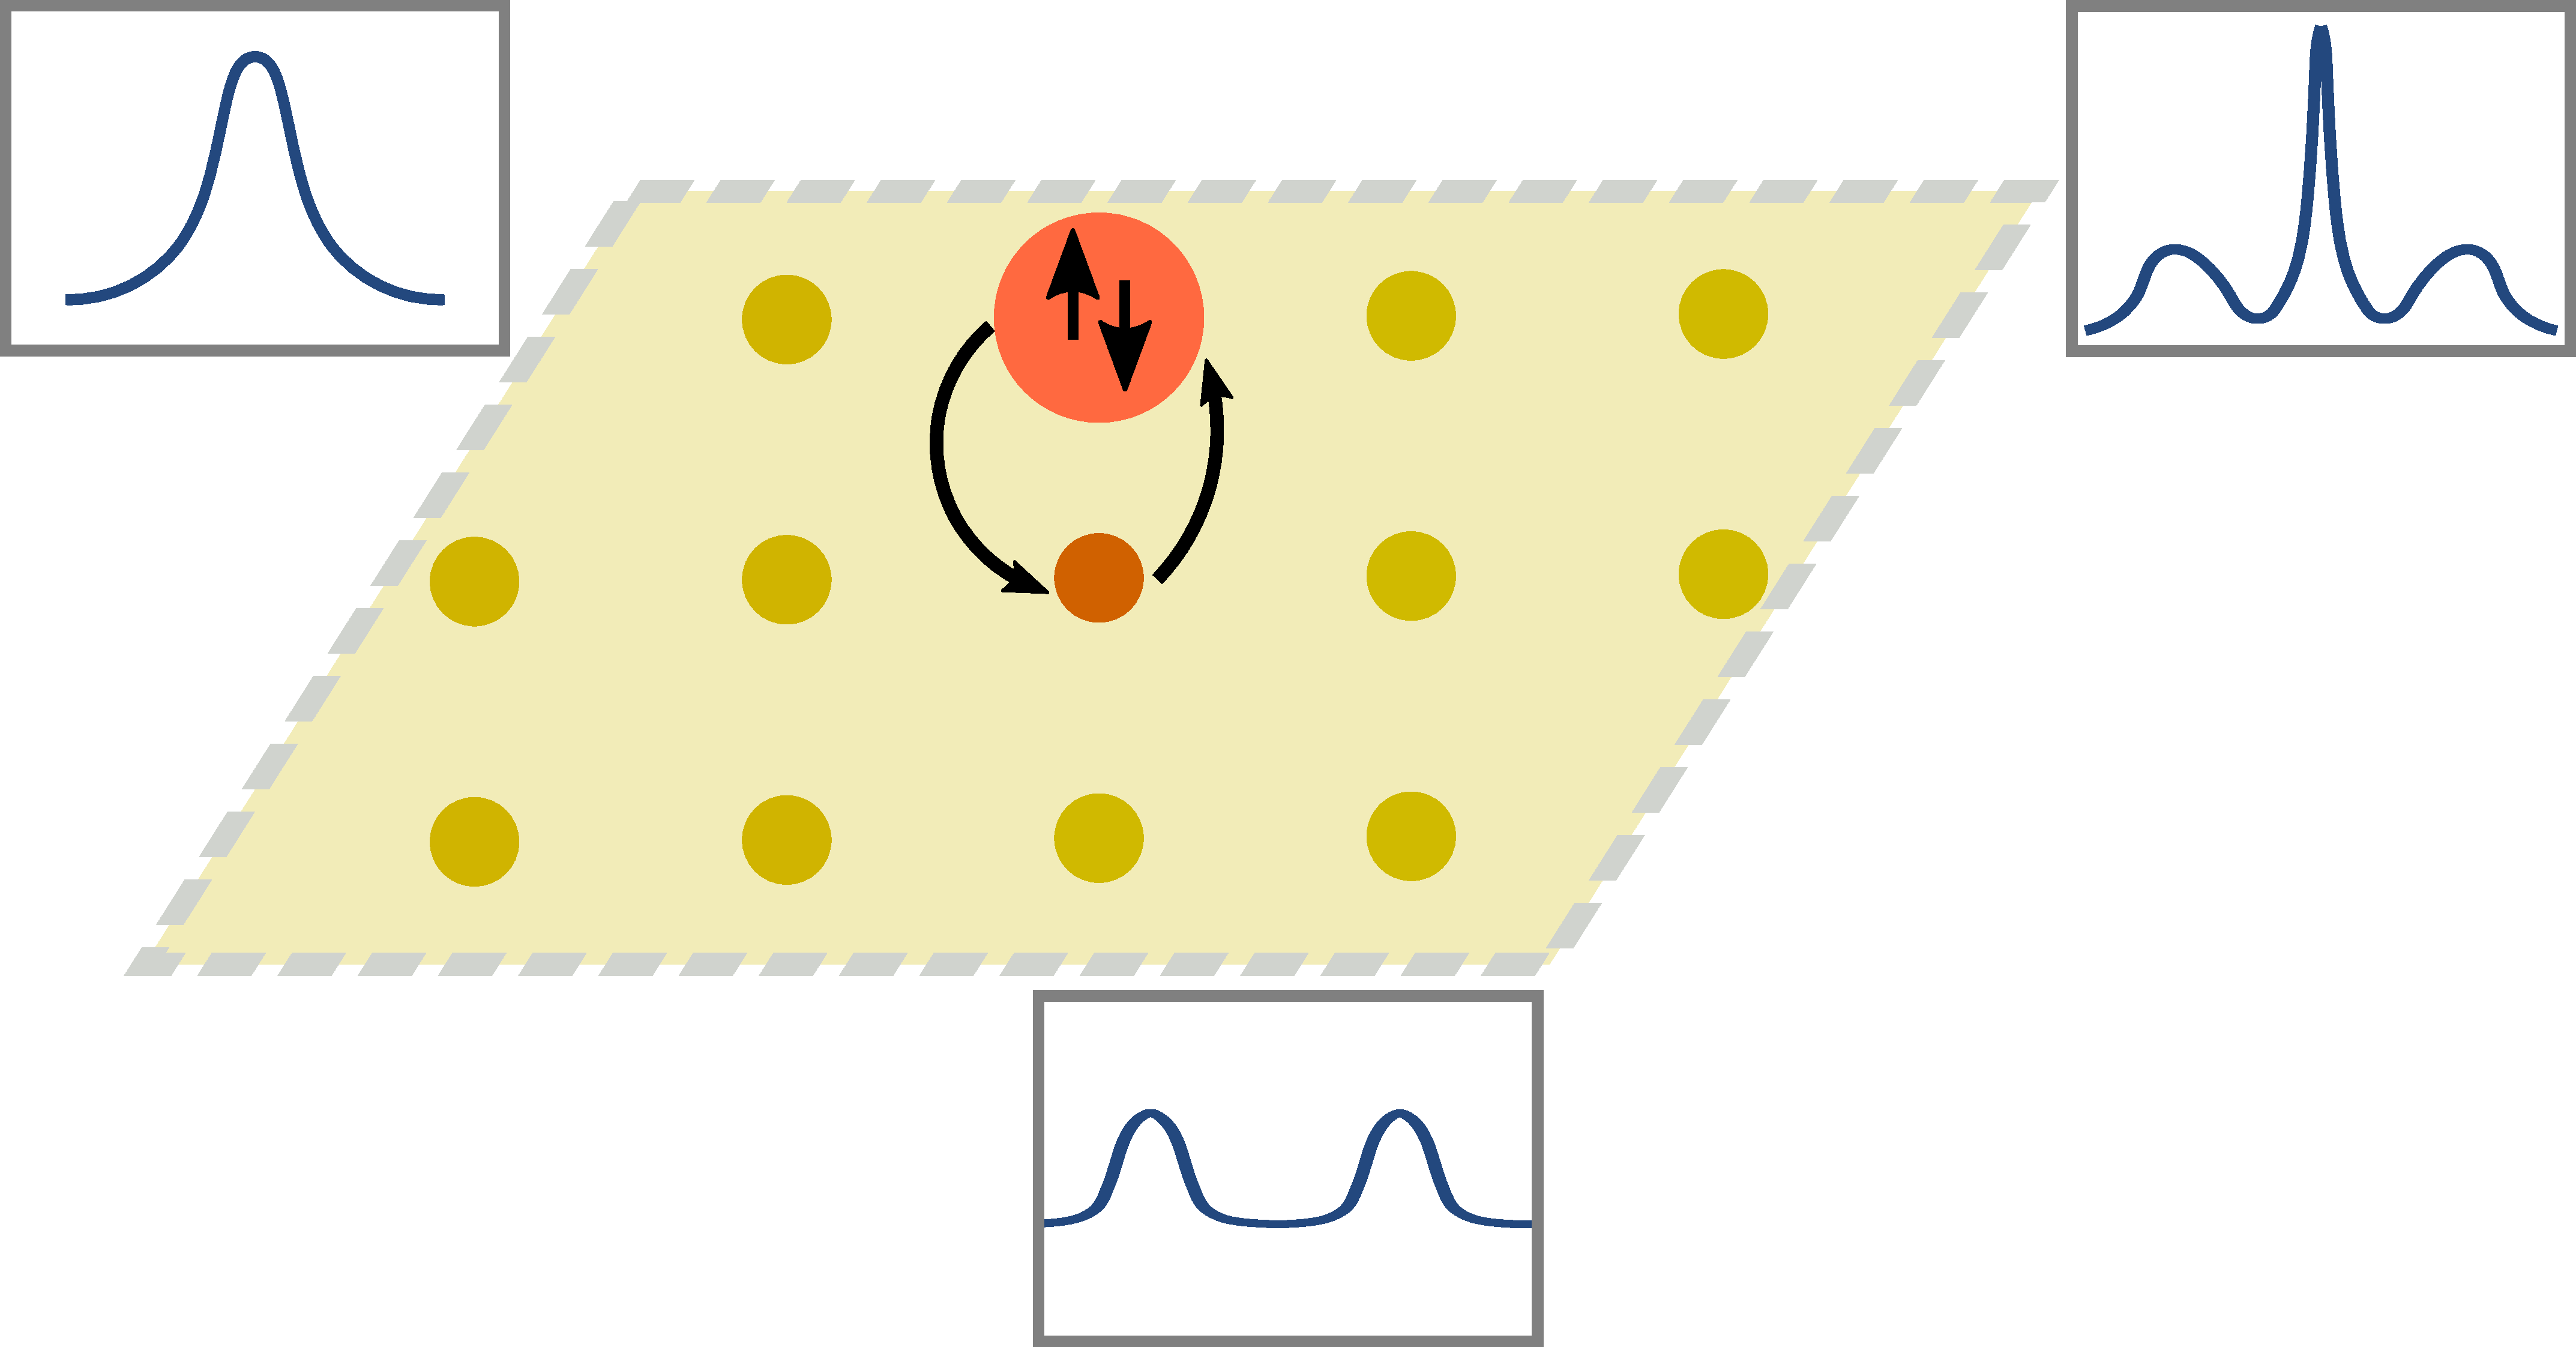
\includegraphics[width=0.8\textwidth]{DMFT.pdf}
\end{minipage}
\hspace*{\fill}
\begin{minipage}{0.45\textwidth}
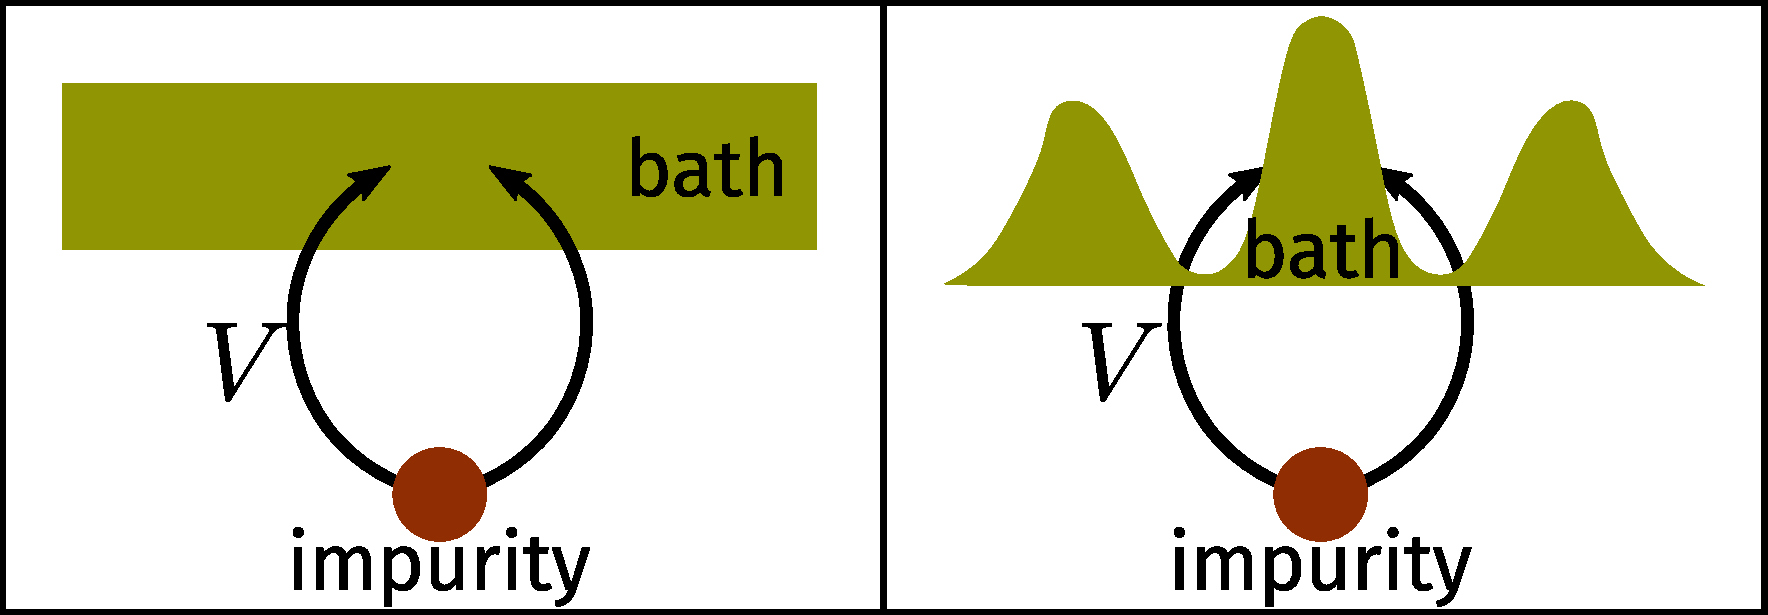
\includegraphics[width=\textwidth]{dos_diff.pdf}
\end{minipage}

\end{frame}

\begin{frame}{}
\section{Introducing the extended Anderson impurity model}
\end{frame}

\begin{frame}{Introducing the extended Anderson impurity model}
\footcite{anderson_1961,anderson_1978,wilson1974,nozieres1974fermi,hrk_wilson_1980,andrei_1980,tsvelickKondoreview,hewson1993,costi_hewson_1990,costi2000,kuramoto1987,Cox1988,metzner_volhardt_1989,kotliar1996,parcollet_2004,maier_2005,kotliar_rmp_2006,ohashi_2008}

\begin{minipage}{0.5\textwidth}
{\bf Standard Anderson impurity model\\}
\begin{itemize}
	\nitem no local-moment phase, \(A(\omega)\) gapless
	\nitem cannot explain insulating phase of DMFT
\end{itemize}
\end{minipage}
\hspace*{\fill}
\begin{minipage}{0.45\textwidth}
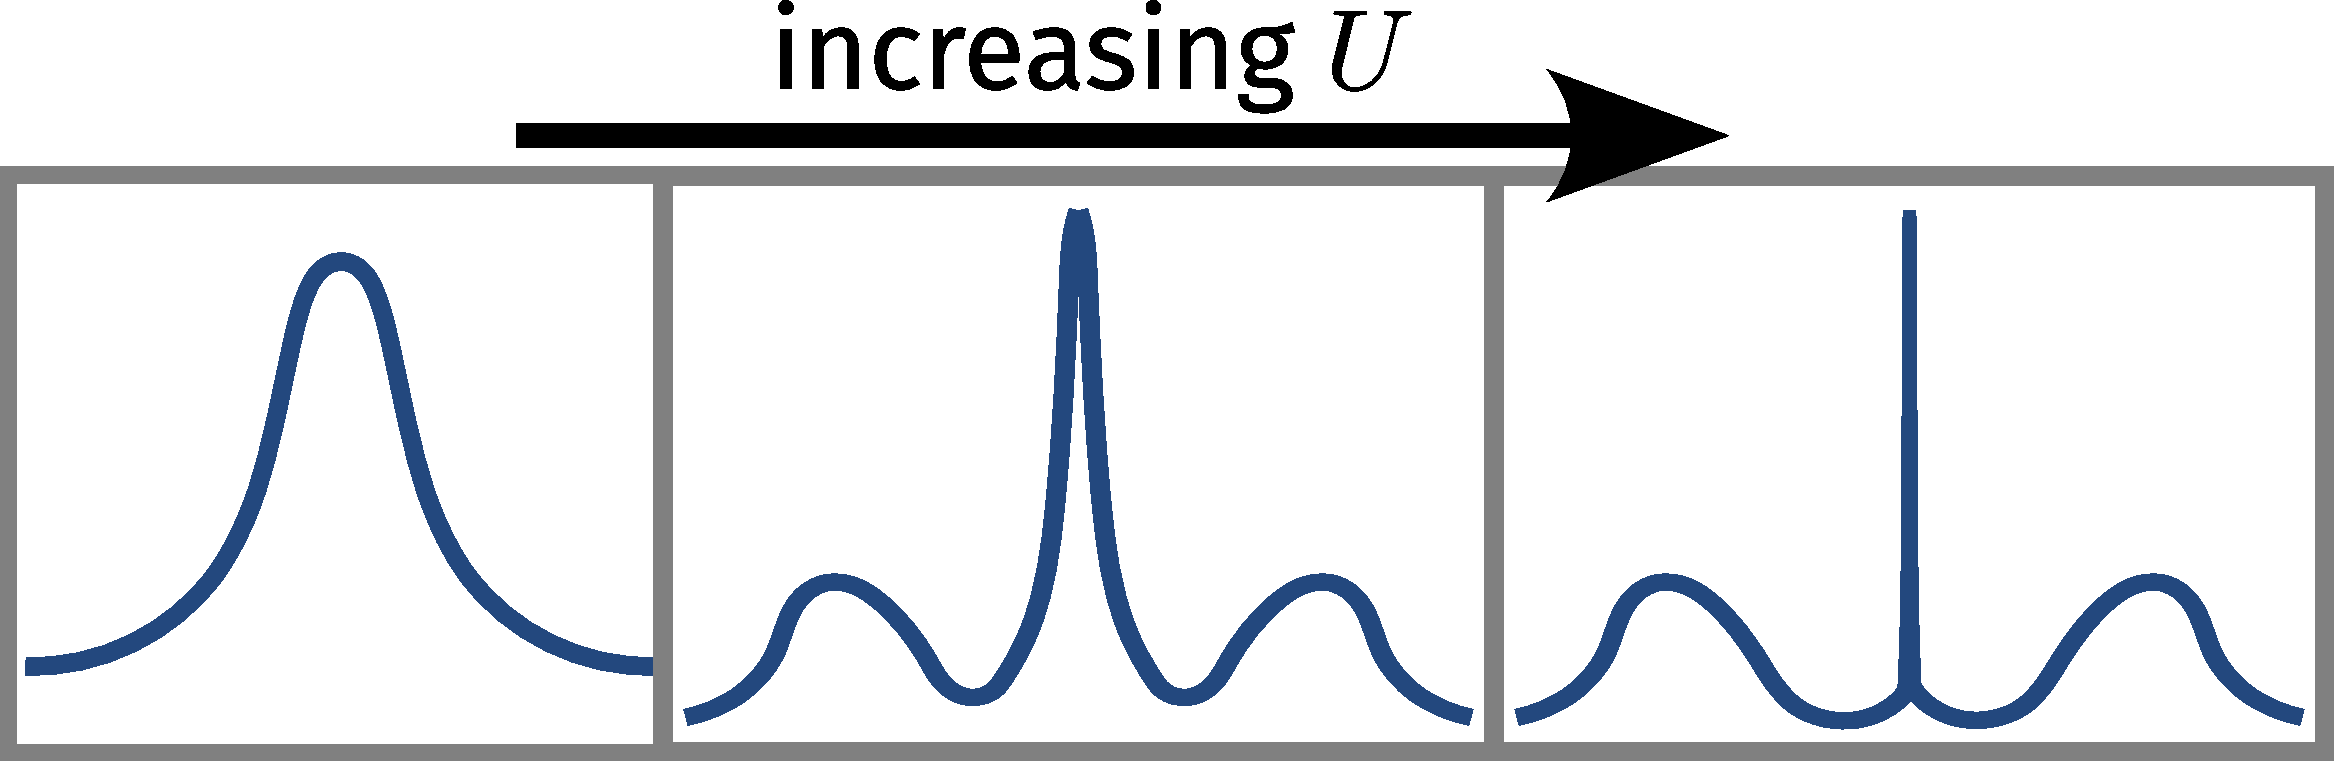
\includegraphics[width=\textwidth]{standard-siam.pdf}
\end{minipage}

\vspace*{20pt}

\alert{Gap in spectral function requires additional physics!}

\vspace*{20pt}

\begin{minipage}{0.5\textwidth}
\textbf{{\it Extended} Anderson impurity model\\}
\begin{itemize}
\nitem impurity-bath spin correlation: \(J\)
\nitem bath zeroth site local correlation: \(U_b\)
\end{itemize}
\end{minipage}
\hspace*{\fill}
\begin{minipage}{0.48\textwidth}
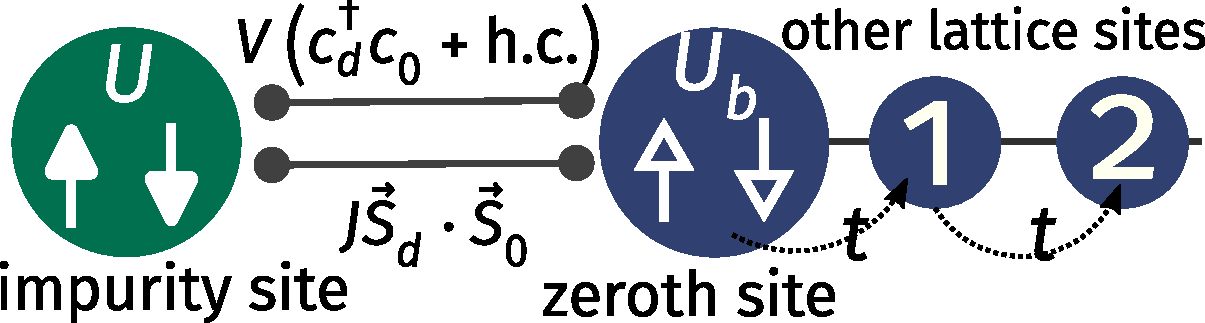
\includegraphics[width=\textwidth]{zeromode_bare.pdf}
\end{minipage}

\end{frame}

\begin{frame}{}
\section{Phase Diagram \& Ground-States}
\end{frame}

\begin{frame}{Nature of RG flows}

\begin{itemize}
\nitem URG Equations reveal \alert{critical} point at  \(r = -U_b / J = 1/4\)\\[10pt]
\nitem allows averting strong-coupling behaviour\\[10pt]
\nitem \(U_b\) always marginal
\end{itemize}

\vspace*{\fill}

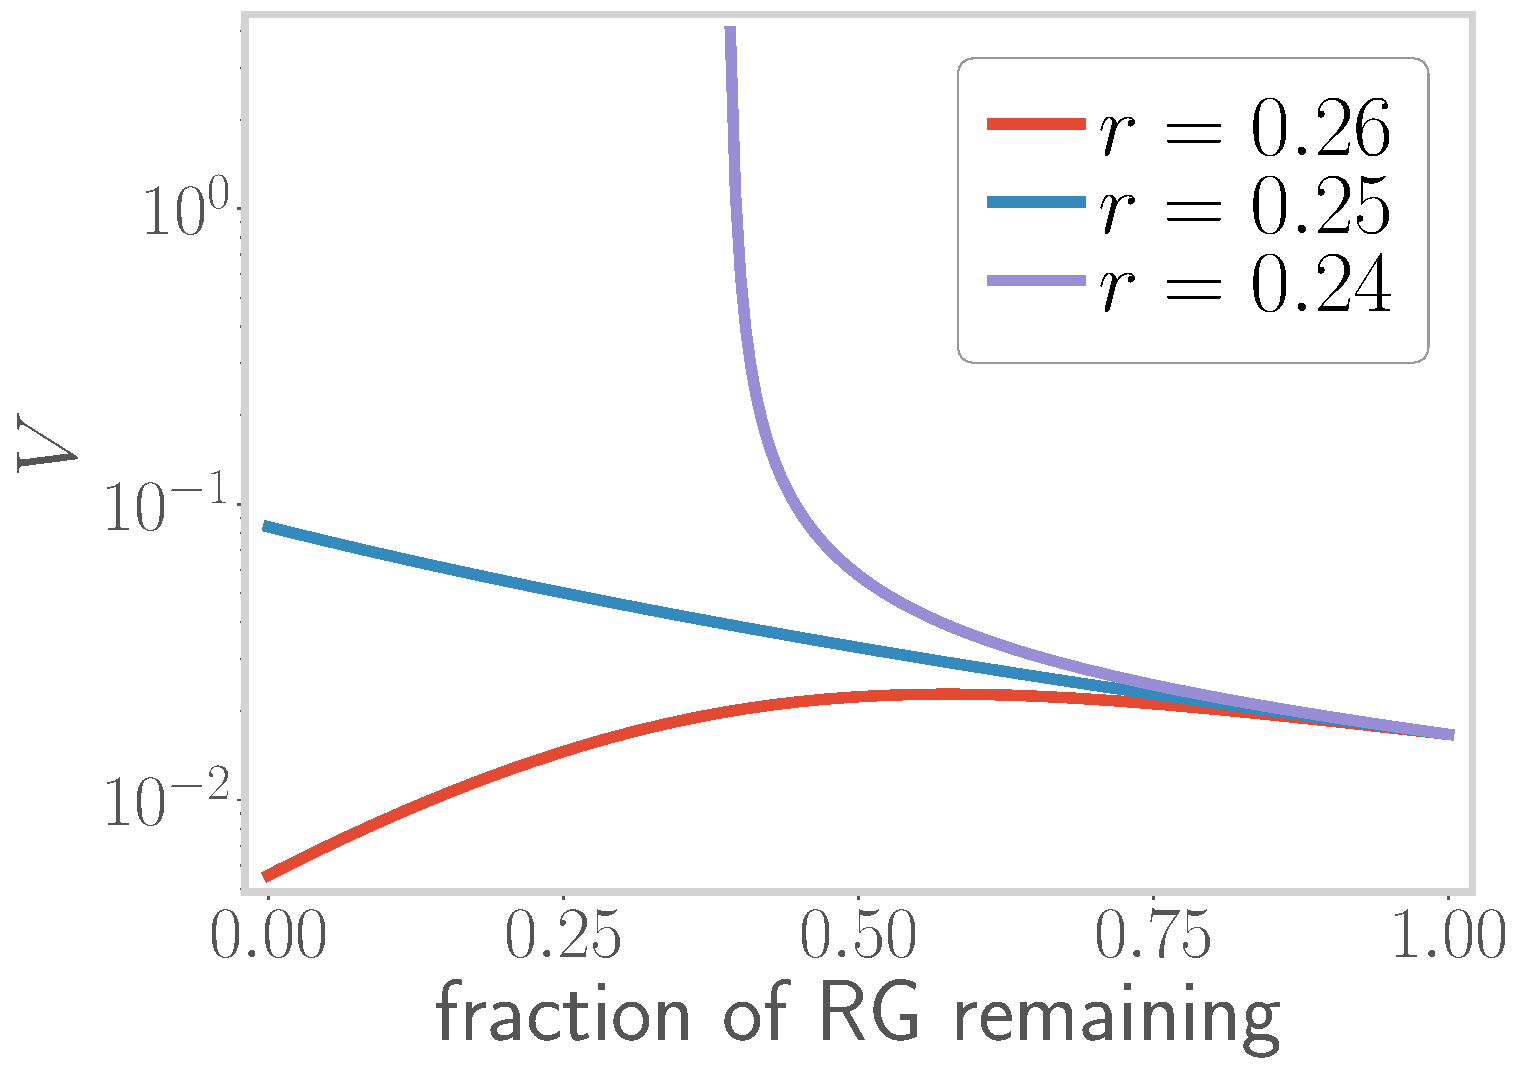
\includegraphics[width=0.45\textwidth]{V_Ub.pdf}
\hspace*{\fill}
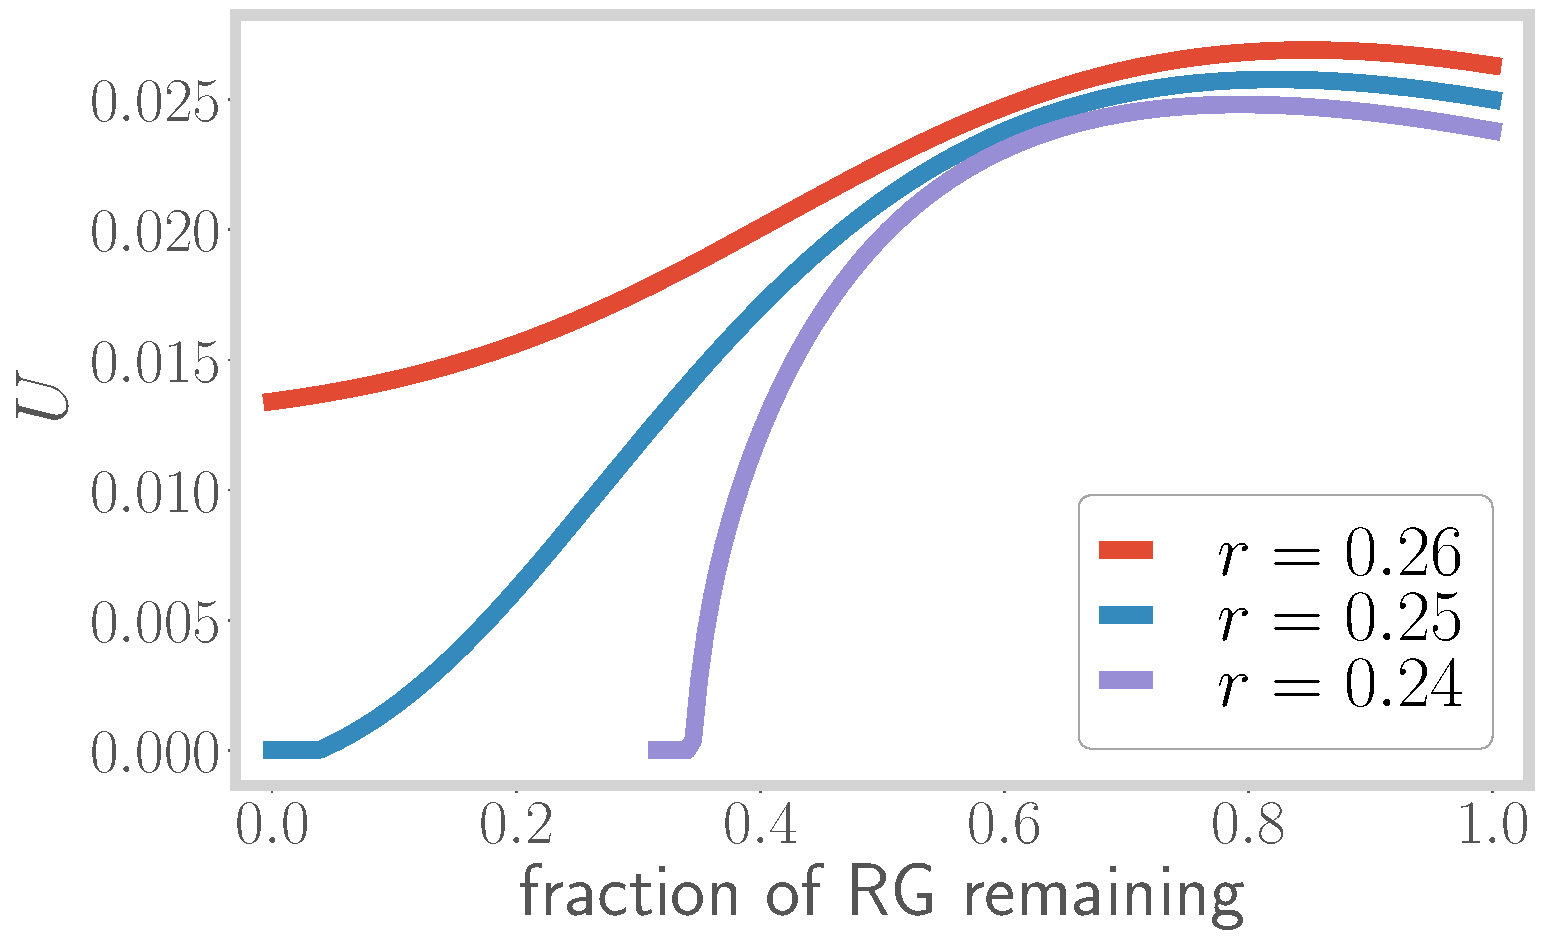
\includegraphics[width=0.45\textwidth]{U_Ub.pdf}

\end{frame}

\begin{frame}{RG Phase Diagram}
\centering

\flushright
\begin{minipage}{0.7\textwidth}
\begin{enumerate}
\nitem blue phase \(\longrightarrow\) \(U_b < -J/4\) : \(V,J\) are \alert{irrelevant} \(\longrightarrow\) local moment flows
\end{enumerate}
\end{minipage}

\vspace*{\fill}

\begin{minipage}{0.45\textwidth}
\begin{enumerate}
\nitem yellow phase: \(J \ll D_0\): involves \alert{\(V,U,U_b\)}\\[5pt]
{\it vanishes for large systems}\\
\vspace*{40pt}
\nitem gray phase: \(J \sim D_0\): \alert{all} couplings irrelevant\\[5pt]
{\it vanishes for large systems}
\end{enumerate}
\end{minipage}
\hspace*{\fill}
\begin{minipage}{0.5\textwidth}
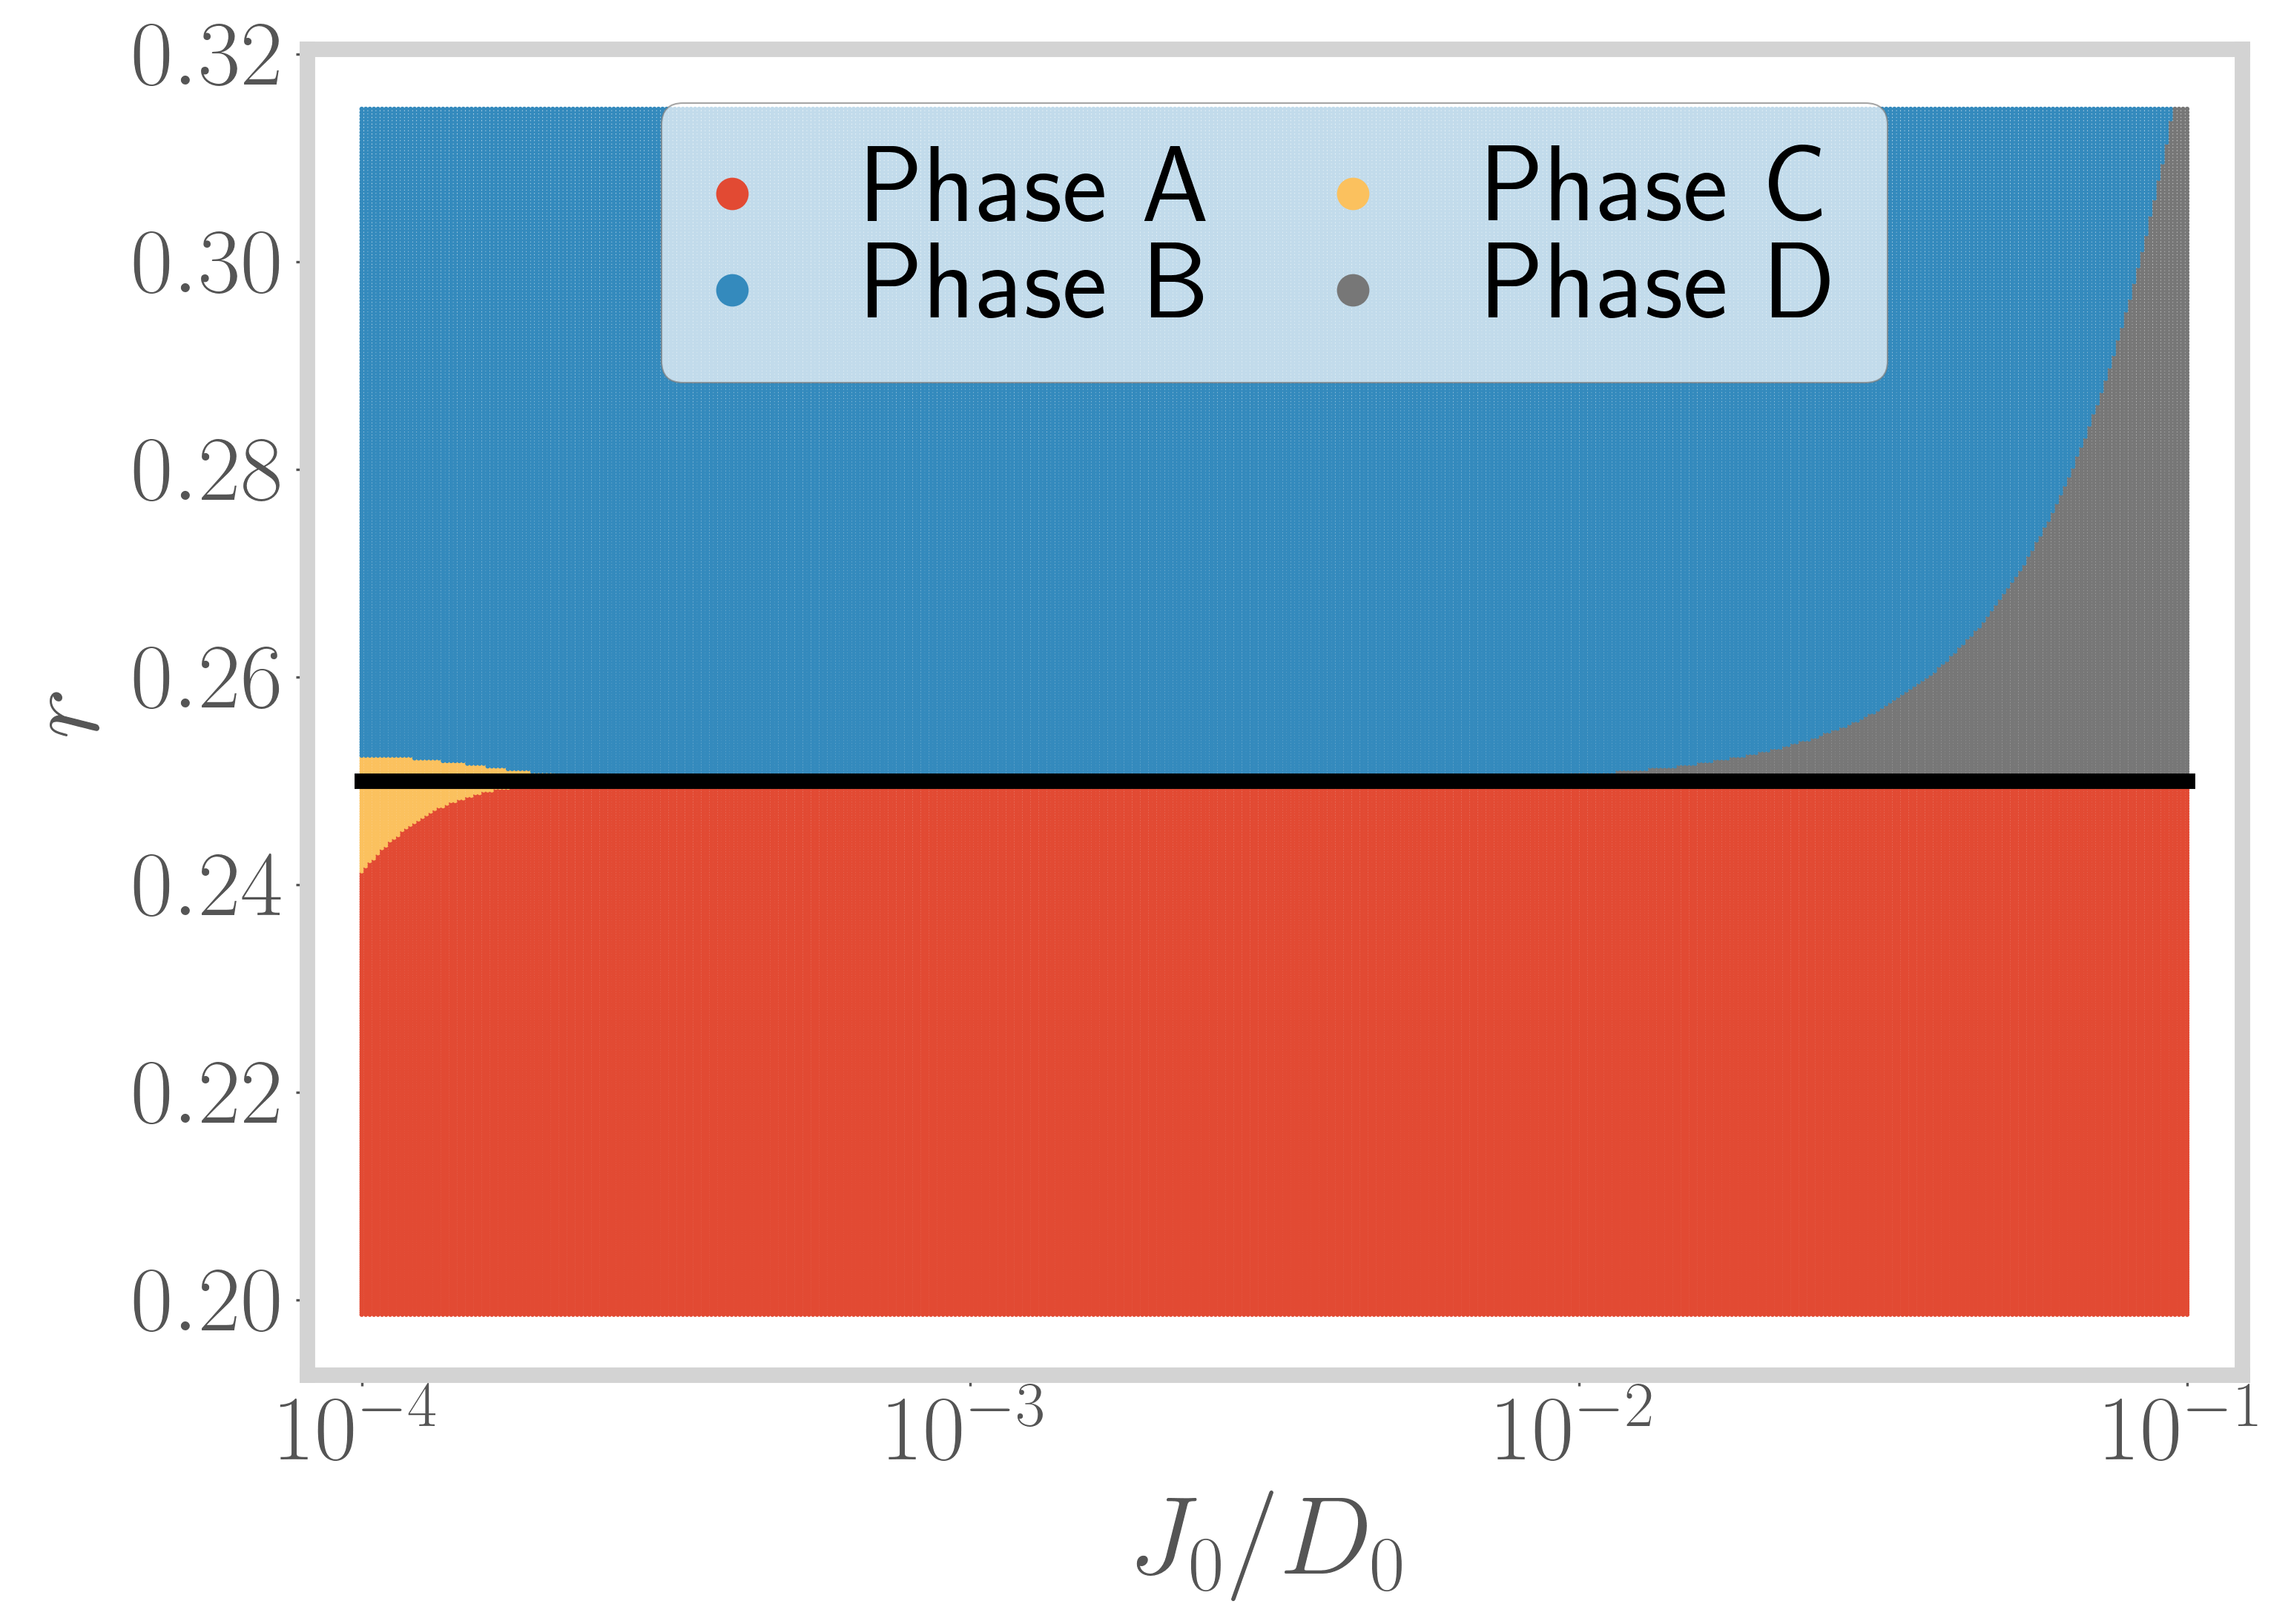
\includegraphics[width=\textwidth]{phase-map-MIT.png}
\end{minipage}

\vspace*{\fill}

\flushright
\begin{minipage}{0.7\textwidth}
\begin{enumerate}
\nitem red phase \(\longrightarrow\) \(U_b > -J/4\): \(V,J\) are \alert{relevant} \(\longrightarrow\) strong-coupling flows
\end{enumerate}
\end{minipage}

\end{frame}

\begin{frame}{Low-energy effective Hamiltonians and ground-states}

\only<1>{
{\Large\underline{\(|U_b| < J/4\)}}\\
\vspace*{\fill}
\begin{minipage}{0.4\textwidth}
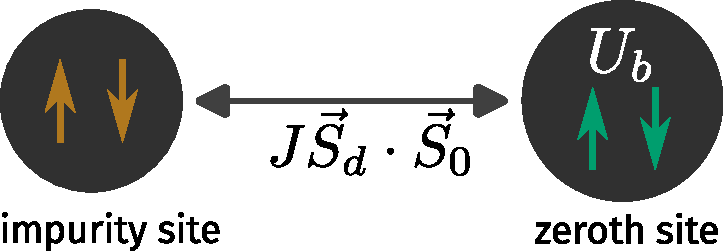
\includegraphics[width=\textwidth]{singlet.pdf}
\end{minipage}
\hspace*{\fill}
\begin{minipage}{0.48\textwidth}
\begin{enumerate}
\nitem two-spin Heisenberg, attractive zeroth site \\[6pt]
\nitem \alert{singlet} ground state
\end{enumerate}
\end{minipage}
}

\only<2>{
{\Large\underline{\(|U_b| \sim J/4\)}}\\
\vspace*{\fill}
\begin{minipage}{0.4\textwidth}
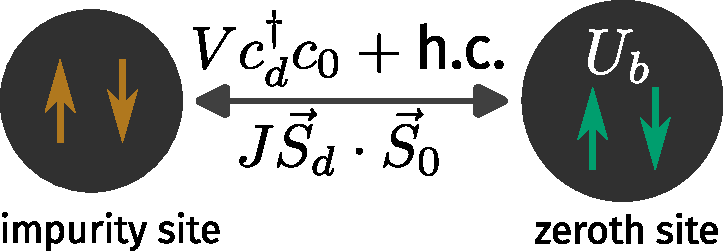
\includegraphics[width=\textwidth]{siam-JV.pdf}
\end{minipage}
\hspace*{\fill}
\begin{minipage}{0.48\textwidth}
\begin{enumerate}
	\nitem \alert{spin+charge} dimer with attractive zeroth site\\[6pt]
\nitem spin-singlet + charge triplet zero in ground state
\end{enumerate}
\end{minipage}
}

\only<3>{
{\Large\underline{\(|U_b| > J/4\)}}\\
\vspace*{\fill}
\begin{minipage}{0.4\textwidth}

\includegraphics[width=\textwidth]{local-moment.pdf}
\end{minipage}
\hspace*{\fill}
\begin{minipage}{0.48\textwidth}
\begin{enumerate}
\nitem impurity site detaches from bath\\[6pt]
\nitem \alert{local moment} ground-state
\end{enumerate}
\end{minipage}
}

\only<4>{
Ground-state overlap with spin singlet and charge triplet zero\\
\vspace*{\fill}
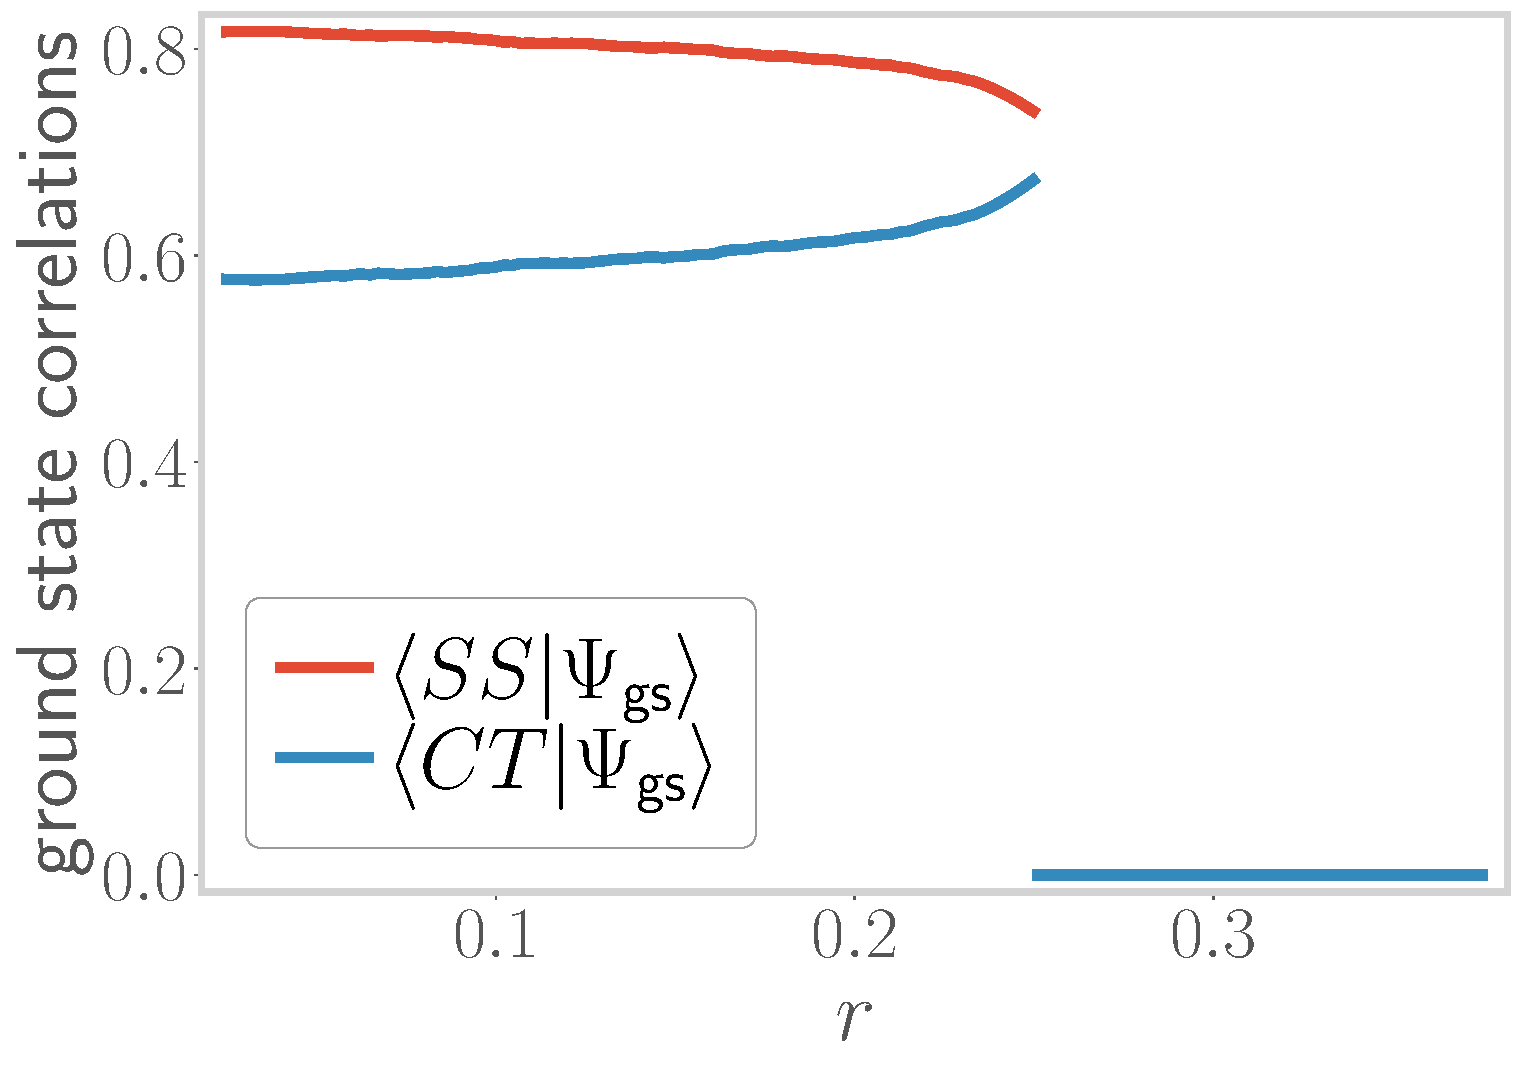
\includegraphics[width=0.6\textwidth]{corrs_gs.pdf}
}
\end{frame}

\begin{frame}{}
\section{Nature of the Transition}
\end{frame}

\begin{frame}{Gapping of the impurity spectral function}
\begin{minipage}{0.25\textwidth}
\begin{itemize}
\nitem Broad central peak at \(|U_b| \ll J/4\)
\end{itemize}
\end{minipage}
\hspace{\fill}
\begin{minipage}{0.45\textwidth}
\begin{itemize}
\nitem Correlated \alert{three peak} structure at \(|U_b| \lesssim J/4\)\\[10pt]
\end{itemize}
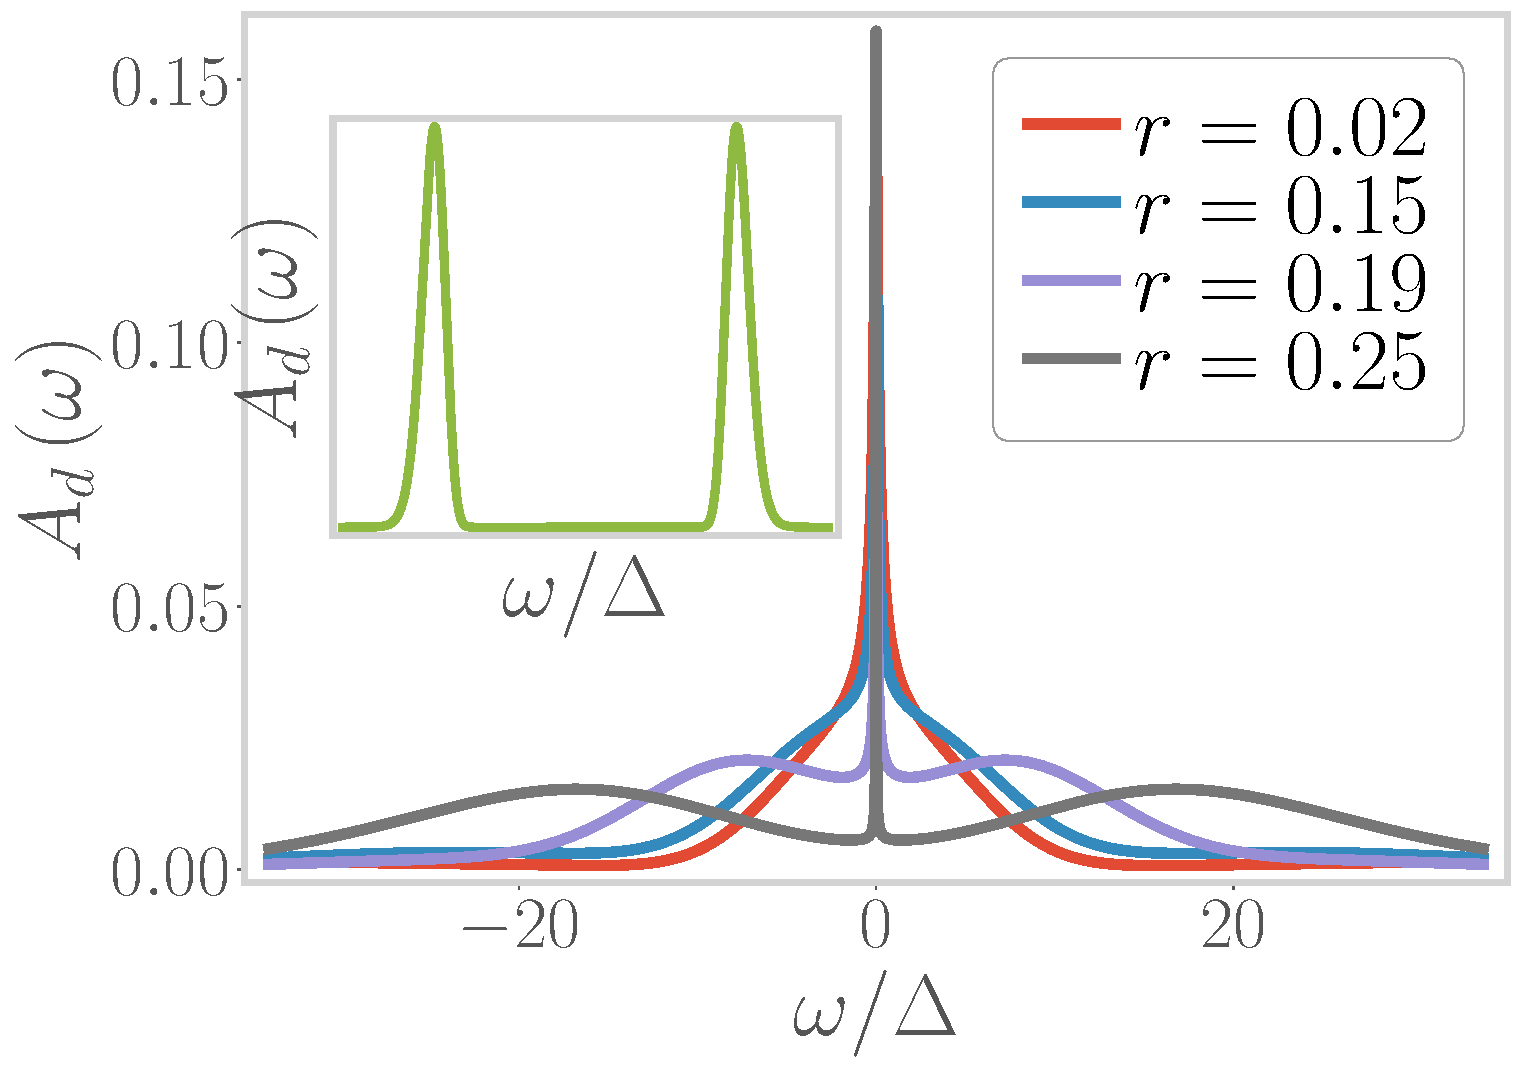
\includegraphics[width=\textwidth]{Add.pdf}
\end{minipage}
\hspace{\fill}
\begin{minipage}{0.25\textwidth}
\begin{itemize}
\nitem hard central \alert{gap} for  \(|U_b| > J/4\)
\end{itemize}
\end{minipage}

\end{frame}

\begin{frame}{Destruction of the Kondo cloud}
\centering
\alert{The Kondo cloud gets destroyed} during the transition.

\vspace*{\fill}

\begin{minipage}{0.4\textwidth}
\begin{itemize}
	\nitem vanishing of impurity-bath correlations
\end{itemize}
\end{minipage}
\hspace*{\fill}
\begin{minipage}{0.4\textwidth}
\begin{itemize}
	\nitem transfer of entanglement into the bath
\end{itemize}
\end{minipage}

\vspace*{\fill}

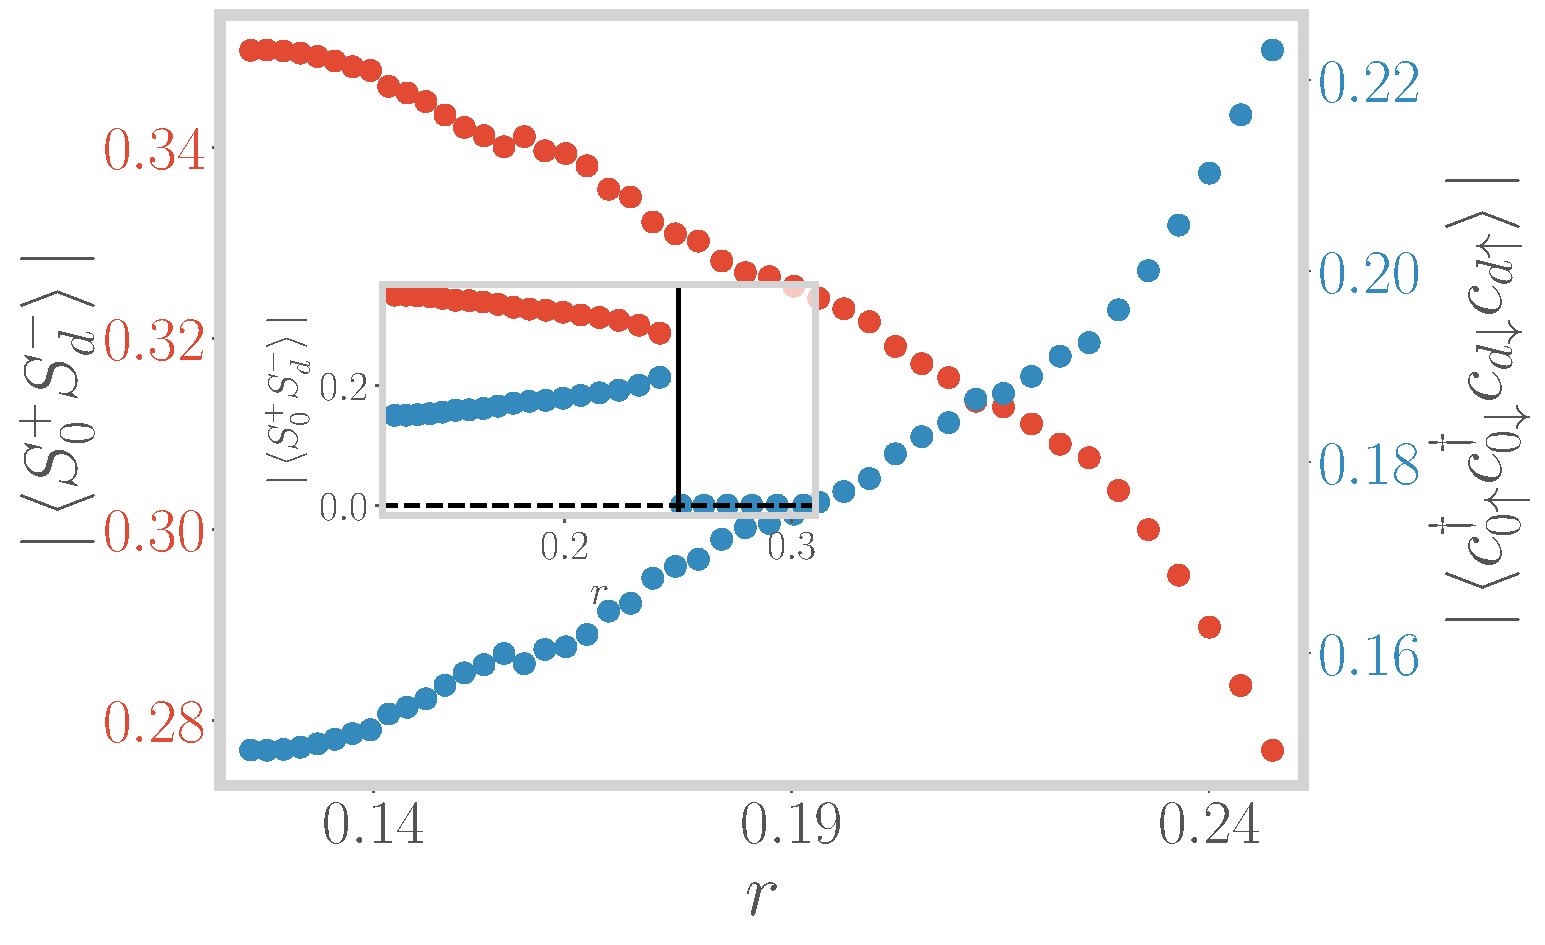
\includegraphics[width=0.45\textwidth]{pairing.pdf}
\hspace*{\fill}
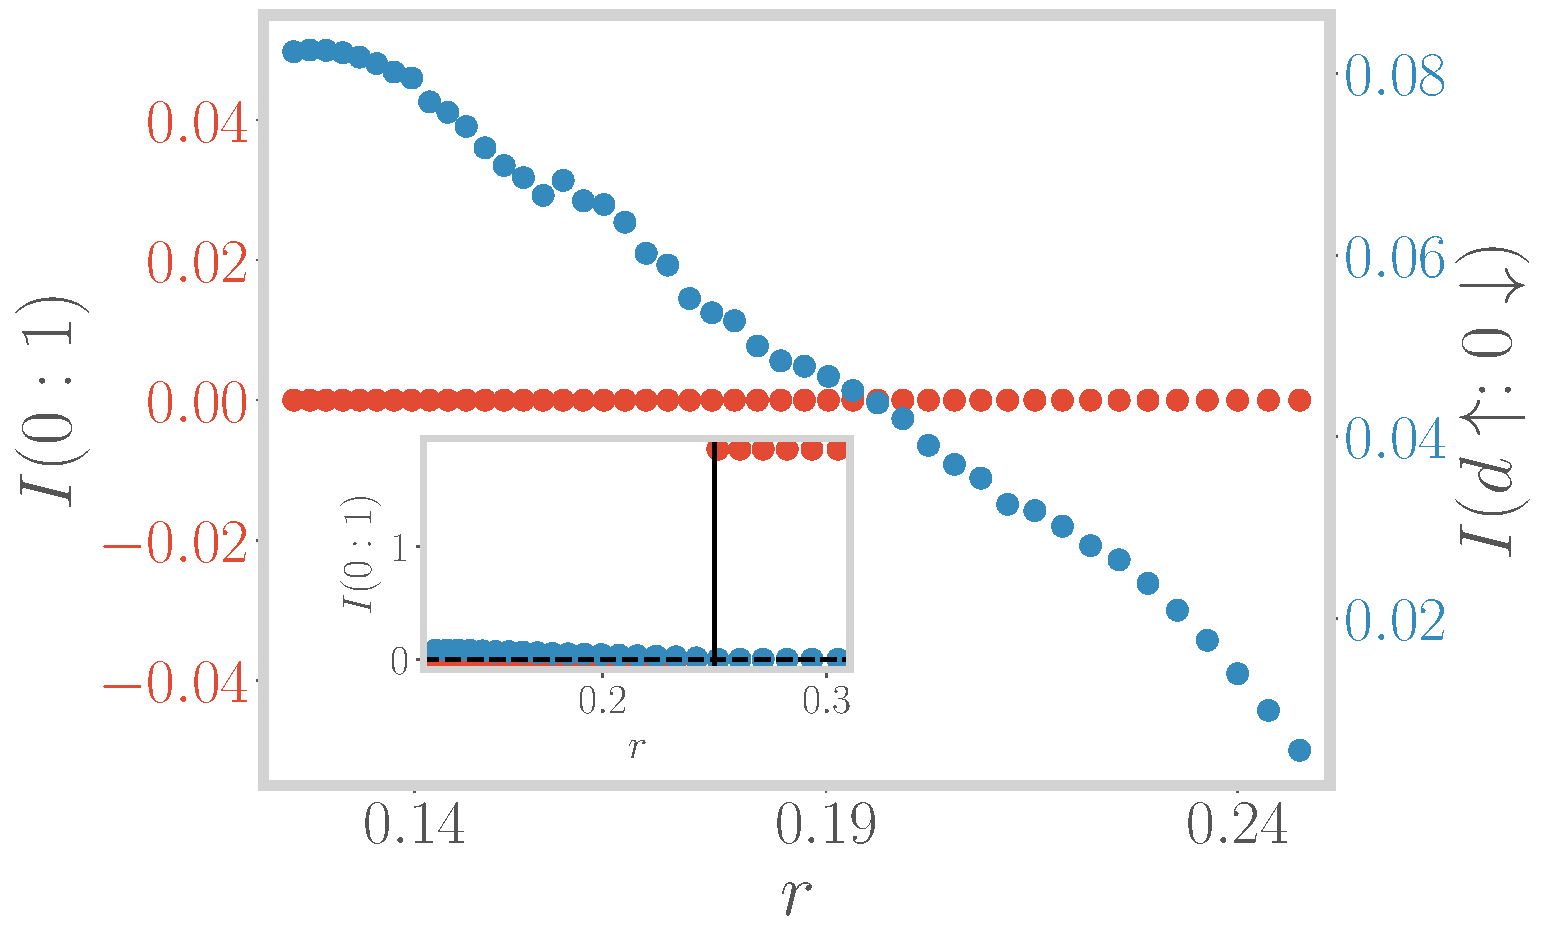
\includegraphics[width=0.45\textwidth]{I_r.pdf}
\end{frame}

\begin{frame}{Growth of pairing fluctuations in the bath}
\centering
\alert{Subdominant pairing fluctuations}, near the transition...

\vspace*{\fill}

\begin{minipage}{0.42\textwidth}
\begin{itemize}
	\nitem growth of fluctuations in Cooper channel, at the cost of spin-flip fluctuations
\end{itemize}
\end{minipage}
\hspace*{\fill}
\begin{minipage}{0.4\textwidth}
\begin{itemize}
	\nitem mutual information within the bath maximised after transition
\end{itemize}
\end{minipage}

\vspace*{\fill}

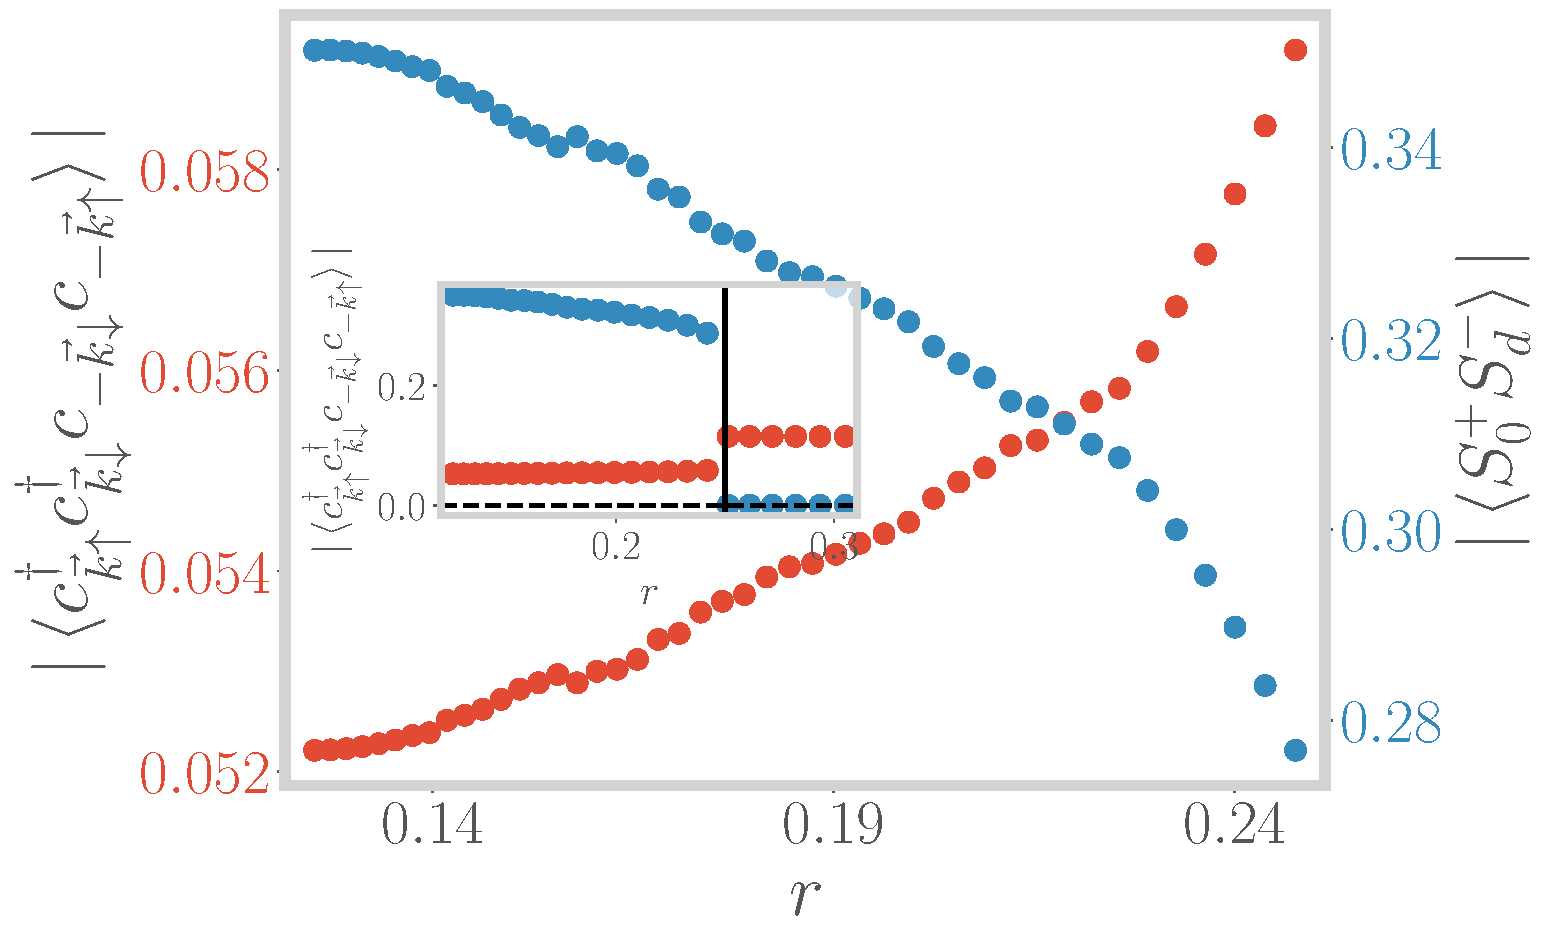
\includegraphics[width=0.45\textwidth]{spinflip-pairing.pdf}
\hspace*{\fill}
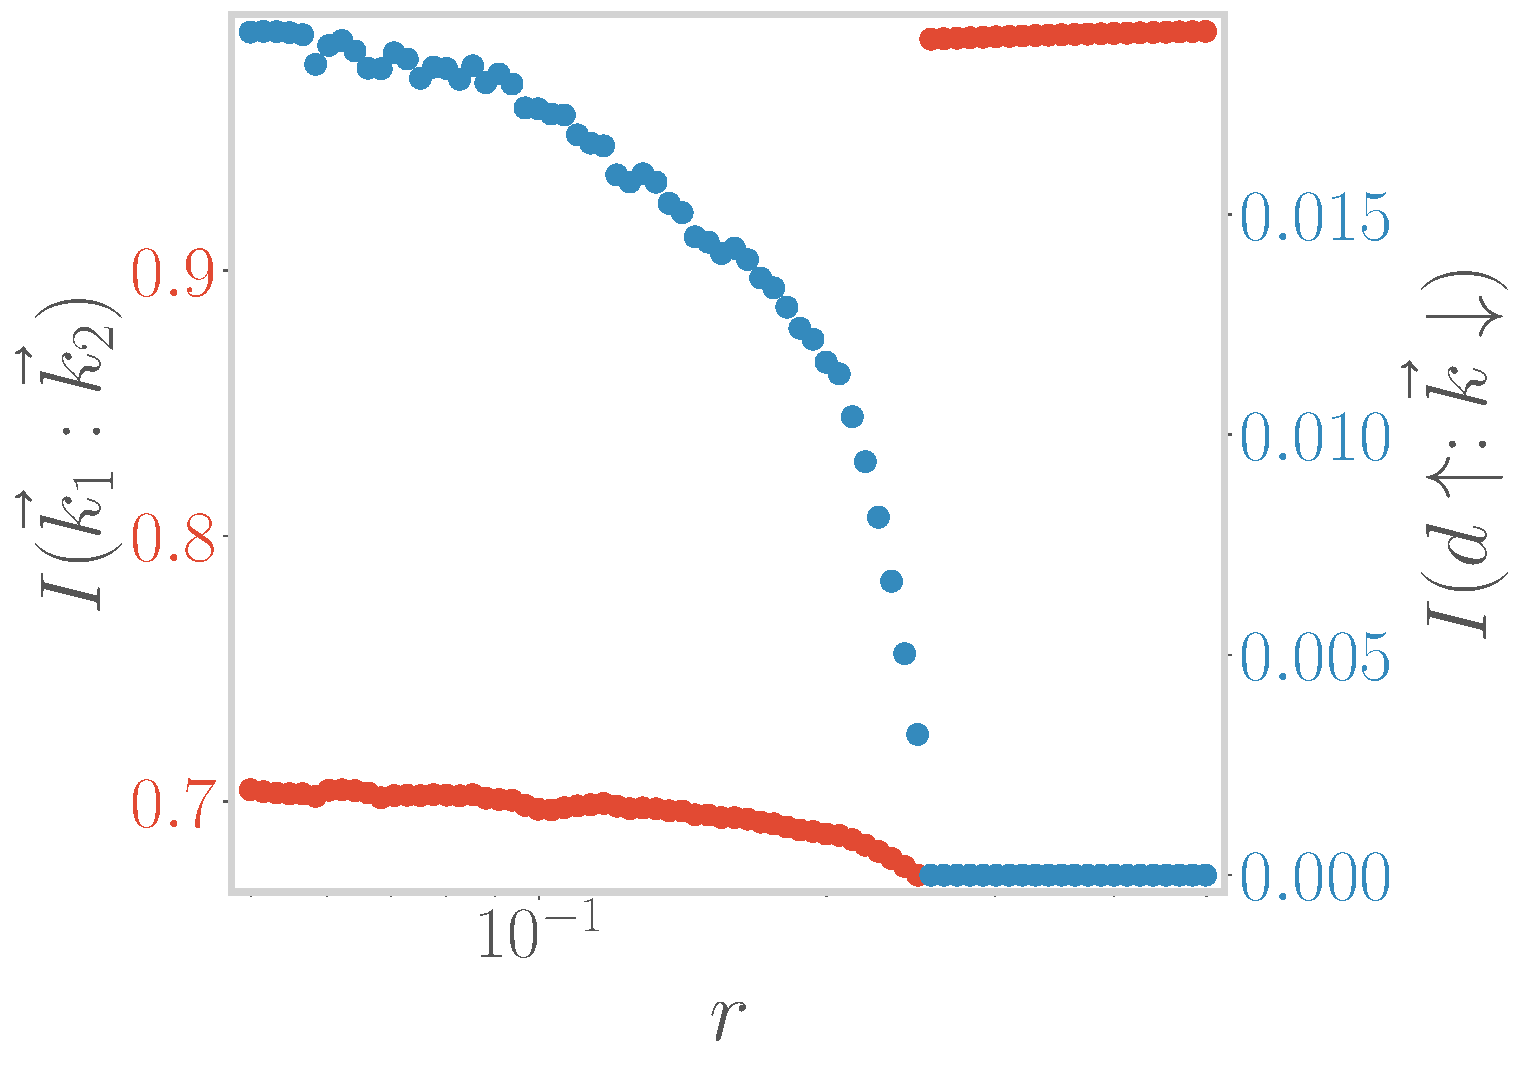
\includegraphics[width=0.45\textwidth]{I_k.pdf}
\end{frame}

\begin{frame}{}
\section{Universal Theory near the Transition}
\end{frame}
\begin{frame}{Minimal effective model for the transition}
\centering
\begin{itemize}
	\nitem For \(|U_b| \lesssim J/4\), central peak and side peaks are \alert{well-separated} \\[10pt]
	\nitem \alert{Integrate out} charge fluctuations through Schrieffer-Wolff transformation
\[H_\text{eff} = \tilde J \vec{S}_d\cdot\vec{S}_0 - U_b\left(\hat n_{0 \uparrow} - \hat n_{0 \downarrow}\right)^2 + H_\text{K.E.}\]
\nitem \alert{captures} the criticality and the strong-coupling and local moment phases
\[ \Delta \tilde J \sim \tilde J \left( \tilde J  + 4U_b \right) \]
\end{itemize}

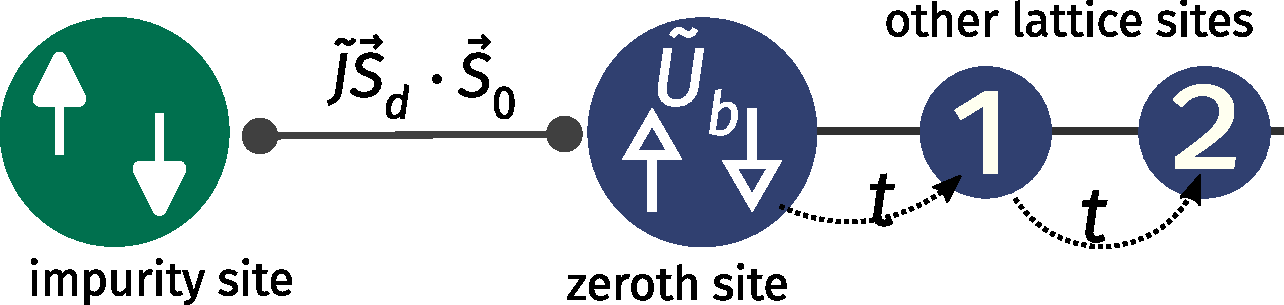
\includegraphics[width=0.6\textwidth]{universal-theory.pdf}

\vspace*{\fill}

Suggests that \alert{$J$ and $U_b$ are the minimal \& universal ingredients} for transition!

\end{frame}

\begin{frame}{Capturing the level crossing at the transition from a two-site model}

\begin{itemize}
	\nitem Obtain two-site model by taking \alert{zero bandwidth} limit\\[10pt]
	\nitem spectrum shows \alert{level crossing} between singlet and local moment states
\end{itemize}

\vspace*{\fill}

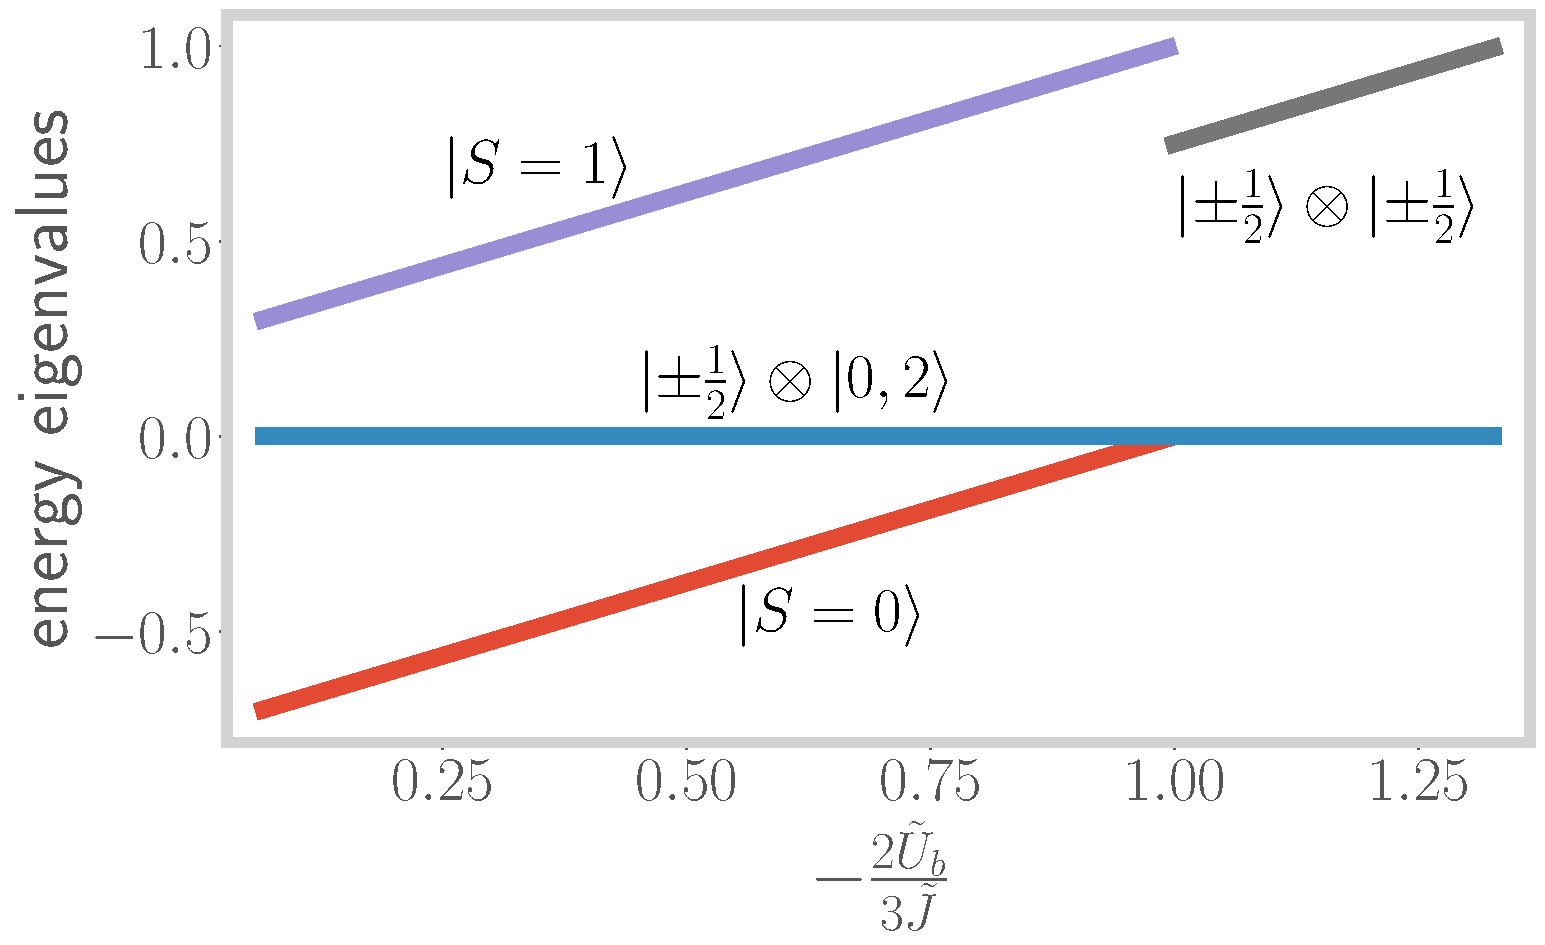
\includegraphics[width=0.5\textwidth]{twosite_spectrum.pdf}
\end{frame}

\begin{frame}{}
\section{Insights into DMFT}
\end{frame}

\begin{frame}{Equivalence of the impurity site and the bath zeroth site}
\begin{itemize}
\only<1>{
	\nitem \alert{Integrate out impurity site} from fixed point Hamiltonian via a single URG transformation\\[10pt]
\nitem Generates additional correlation $U_0$ on zeroth site
\vspace*{\fill}
\begin{center}
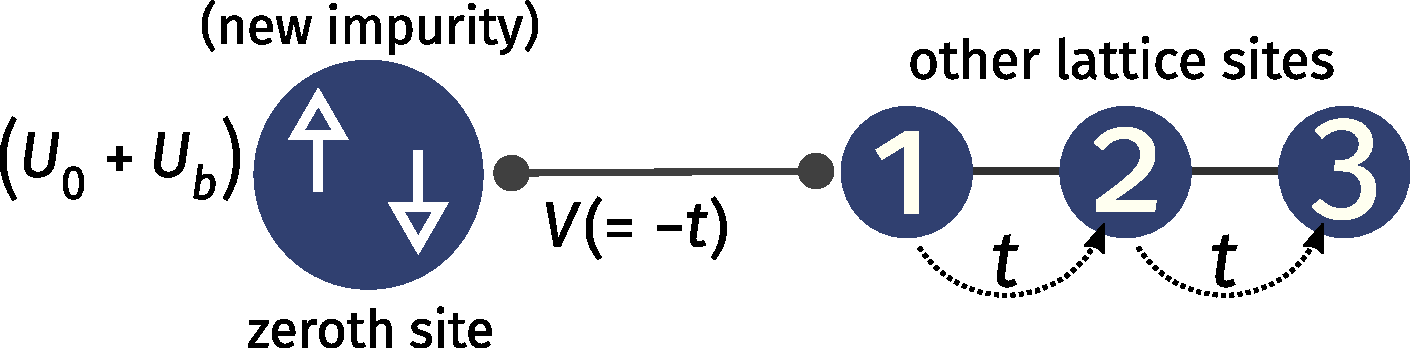
\includegraphics[width=0.6\textwidth]{decouple-impurity.pdf}
\end{center}
}
\only<2>{
	\nitem \(J\) is relevant and the largest scale \(\longrightarrow\) \alert{repulsive correlation}:
	\[U_0 + U_b \simeq J > 0\]
\nitem \(J\) acts a \alert{symmetrisation mechanism} between impurity and zeroth sites\\[10pt]
\nitem \alert{Coherent} spin-flip scatterings ensure similarity of spectral functions
}
\end{itemize}
\vspace*{\fill}
Essence of \alert{self-consistency}: Equivalence of impurity and zeroth sites!
\end{frame}


\begin{frame}{Observation of a coexistence region}
\only<1>{
\begin{itemize}
	\nitem DMFT observes a \alert{coexistence region} near the critical point, for \(U_{c1} < U < U_{c2}\)\\
\begin{center}
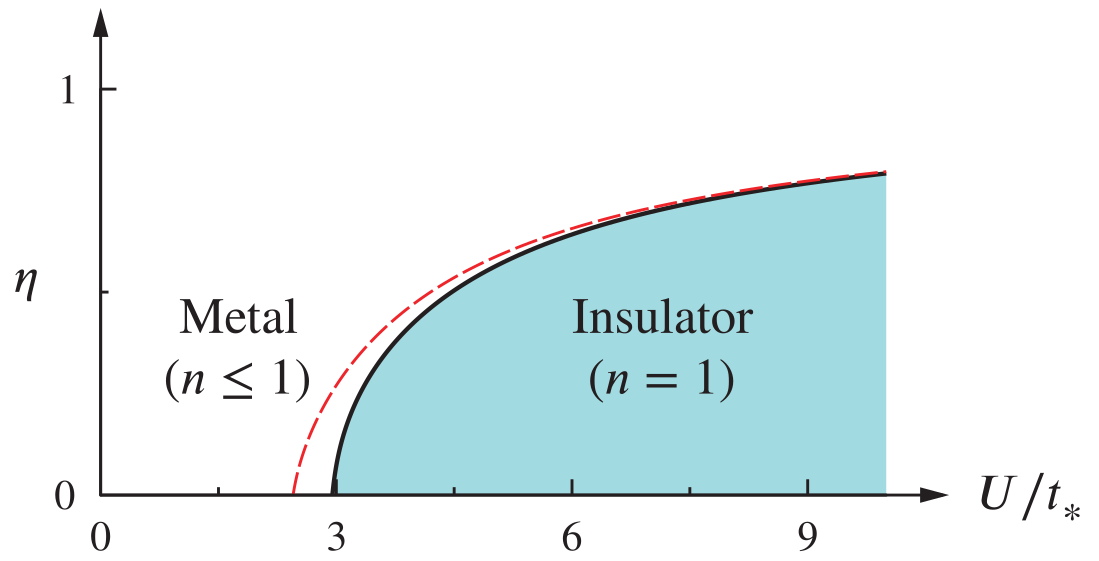
\includegraphics[width=0.5\textwidth]{coexistence.png}\\
\footnotesize{(D.E. Logan and M.R Galpin 2016 JPCM 28 025601) }\\[10pt]
\end{center}
\nitem Insulating when coming in from the insulator, metallic when coming in from the metal\\[10pt]
\nitem True transition believed to occur at \(U_{c2}\)
\end{itemize}
}
\only<2->{
\alert{Can be explained} heuristically using the two site spectrum\\[10pt]
\vspace*{\fill}
\begin{itemize}
\only<2>{\nitem Initial point is when the side peaks get separated (near-zeroes in the spectral function)}
\only<3>{\nitem \(U_{c2}\) is the point where the levels cross}
\only<4>{\nitem Coming from \(U > U_{c2}\), \alert{adiabatic continuity} allows DMFT to stay on the local moment state...}
\only<5>{\nitem For \(U < U_{c1}\), local moment state is too unstable, \alert{relaxes} to the true ground state.}
\end{itemize}

\vspace*{\fill}
\begin{center}
\only<2>{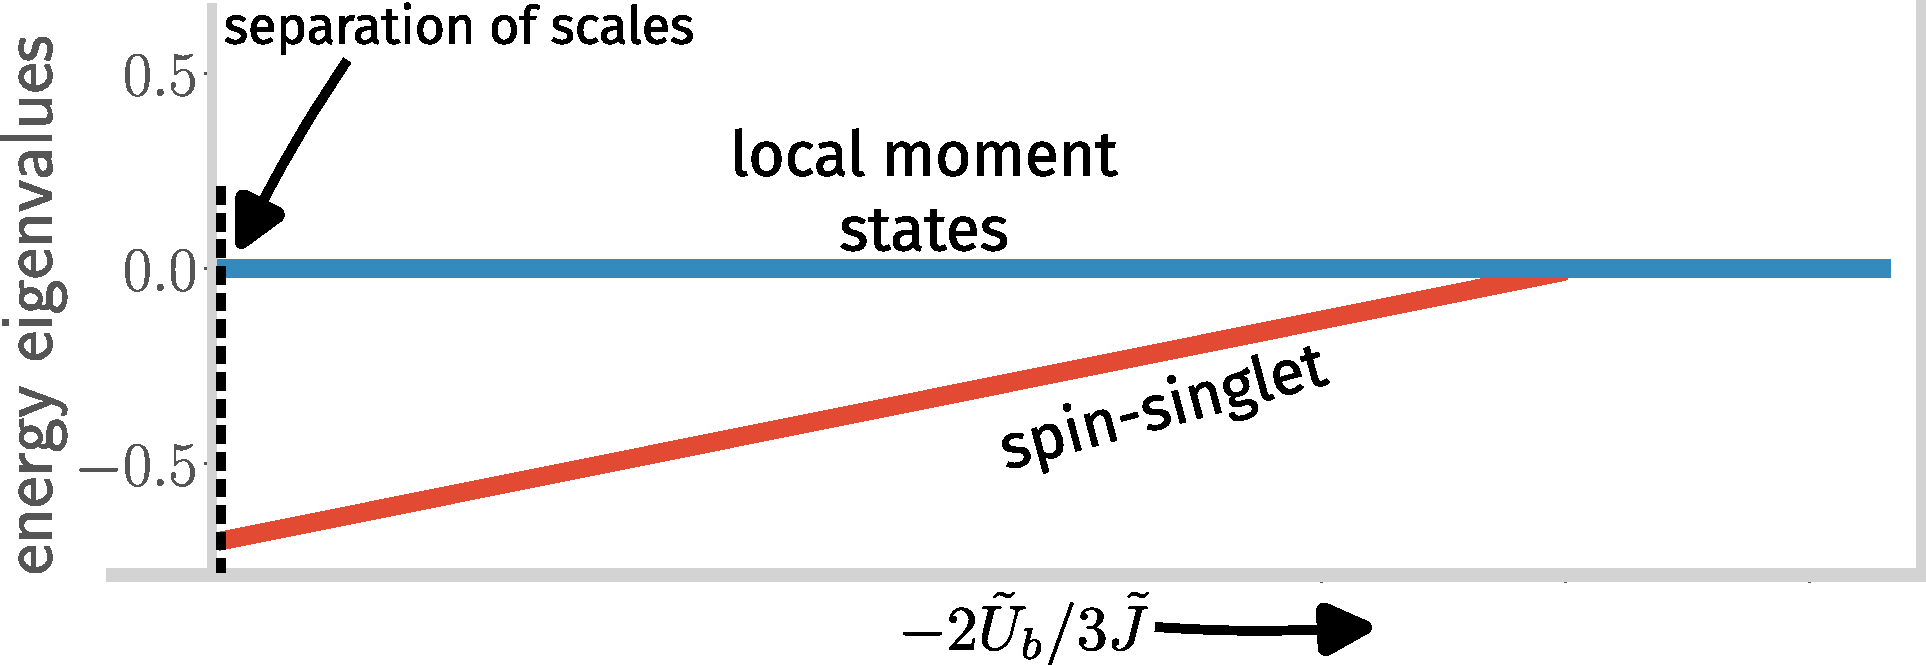
\includegraphics[width=0.7\textwidth]{coexistence-explain.pdf}}
\only<3>{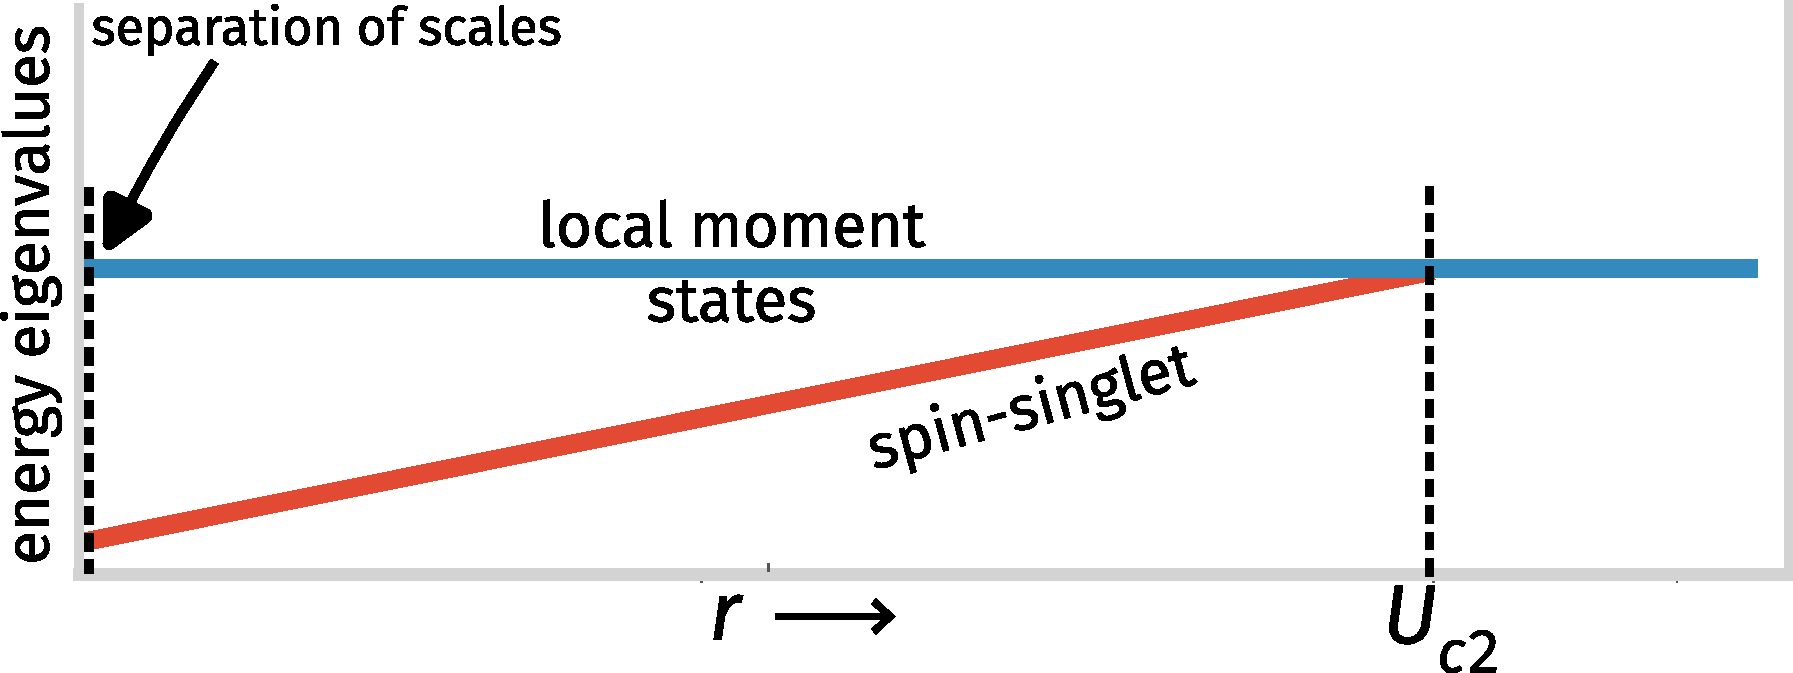
\includegraphics[width=0.7\textwidth]{coexistence-explain1.pdf}}
\only<4>{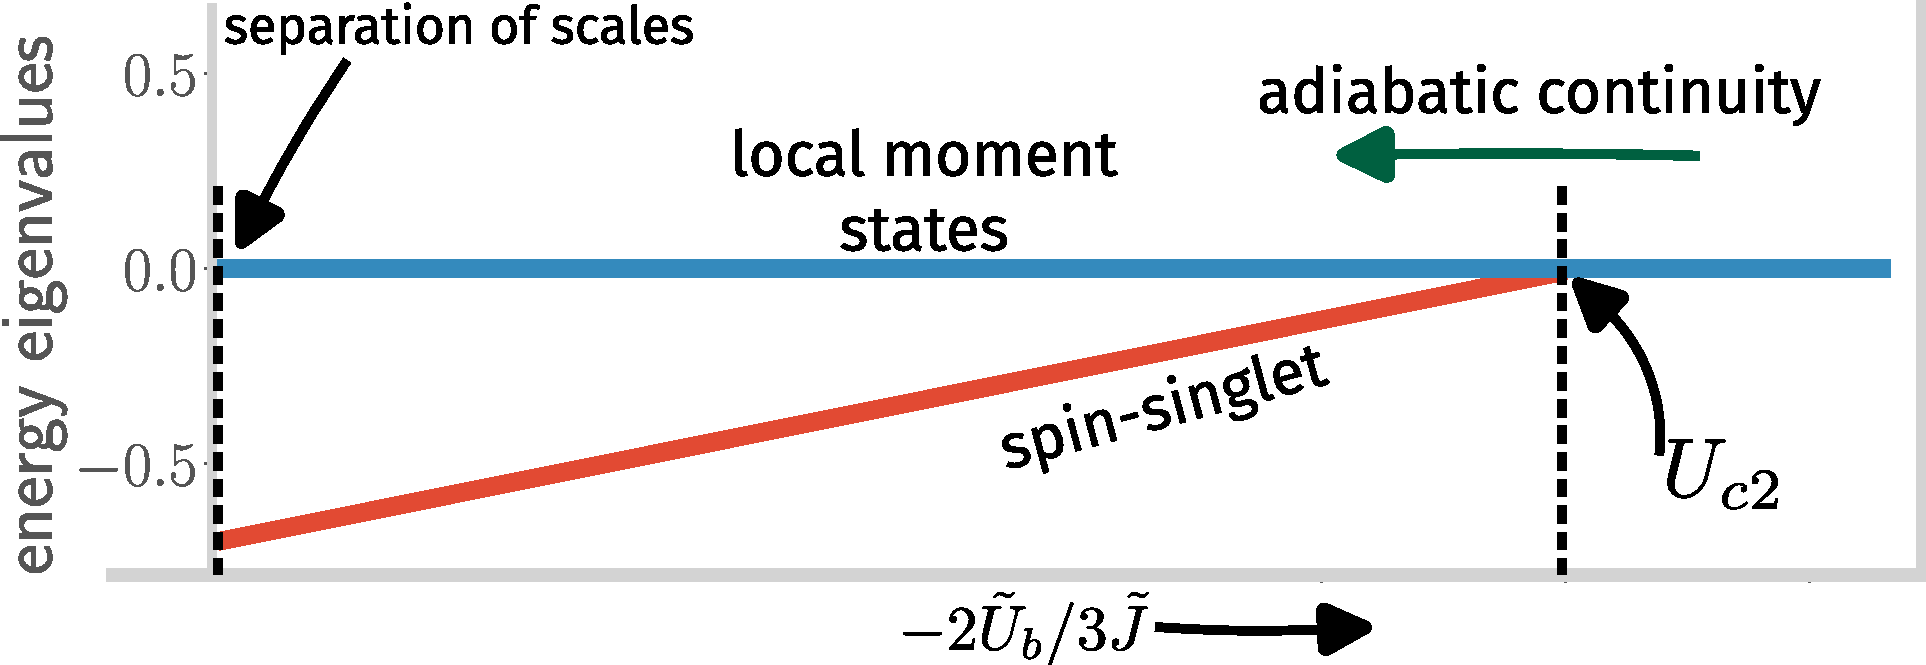
\includegraphics[width=0.7\textwidth]{coexistence-explain2.pdf}}
\only<5>{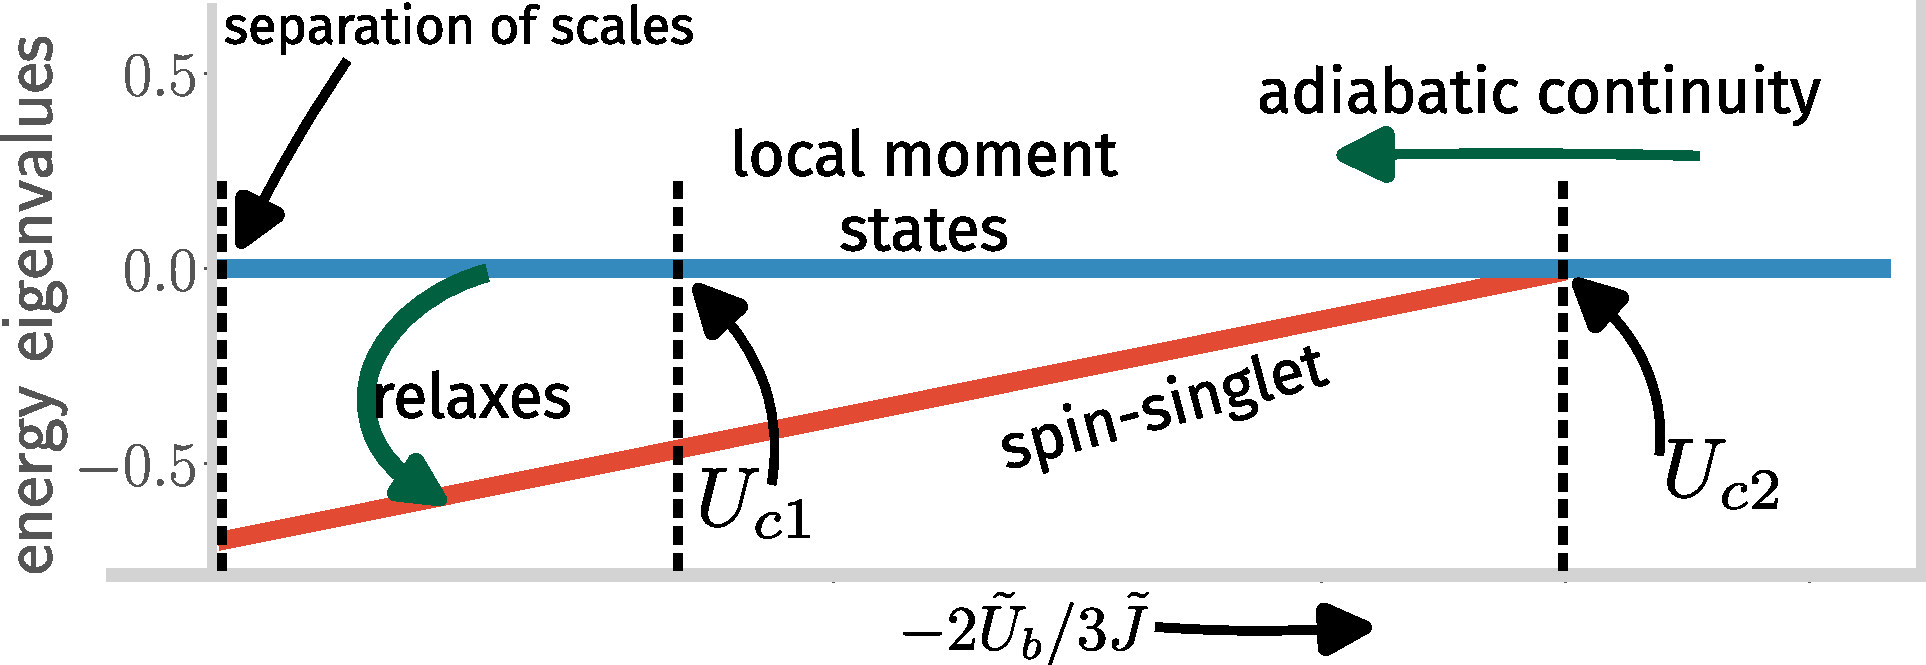
\includegraphics[width=0.7\textwidth]{coexistence-explain3.pdf}}
\end{center}
}
\end{frame}


\begin{frame}{Comparison of correlation functions}
held-toshi and lee-von delft
\end{frame}

\begin{frame}{}
\section{Low-energy excitations of the bath}
\end{frame}
\begin{frame}{effective Hamiltonian for the excitations of the bath near the transition}
\end{frame}
\begin{frame}{emergence of NFL terms at the critical point}
\end{frame}

\begin{frame}{}
\section{Future Prospects}
\end{frame}

\begin{frame}{Future Prospects}
\begin{itemize}
	\nitem Better model can be obtained by taking multiple impurities and general impurity filling\\[20pt]
\nitem novel auxiliary model method can used for studying other models of strong-correlations as well as topologically active or flat band systems\\[20pt]
\nitem The URG can be applied to heavy-fermion materials towards a study of phase diagram and unconventional superconductivity, as well as Kondo insulators\\[20pt]
\nitem Interacting systems in a magnetic field is also a potential area of study, specifically fractional Chern insulators (e.g. the fractional quantum hall effects)
\end{itemize}
\end{frame}


\begin{frame}{Acknowledgements}

\flushleft
Gracious thanks to\\[10pt]
\begin{itemize}
	\nitem my collaborators \alert{S. Patra, A. Mukherjee, Prof. A. Taraphdar} and \alert{Prof. N. S. Vidhyadhiraja},\\[10pt]
	\nitem \alert{Prof. Ritesh Singh} and \alert{Prof. Anandamohan Ghosh} for instructive feedback,\\[10pt]
	\nitem \alert{Prof. H. Casini, Prof. N. Banerjee} and \alert{Shibendu G. Chowdhury} for very fruitful discussions, and\\[10pt]
	\nitem IISER Kolkata for funding.
\end{itemize}

\end{frame}

\appendix

\begin{frame}[allowframebreaks]{References}
\printbibliography[heading=none]
\end{frame}

\begin{frame}{}
\section{Further Details}
\end{frame}

\begin{frame}{}
\section{Theory for the single-channel Kondo cloud}
\begin{minipage}{0.55\textwidth}
	\small{{\bf Phys. Rev. B 105, 085119}\\[10pt]
Anirban Mukherjee, \alert{Abhirup Mukherjee}, N. S. Vidhyadhiraja, A. Taraphder, and Siddhartha Lal}
\end{minipage}
\hspace*{\fill}
\begin{minipage}{0.4\textwidth}
	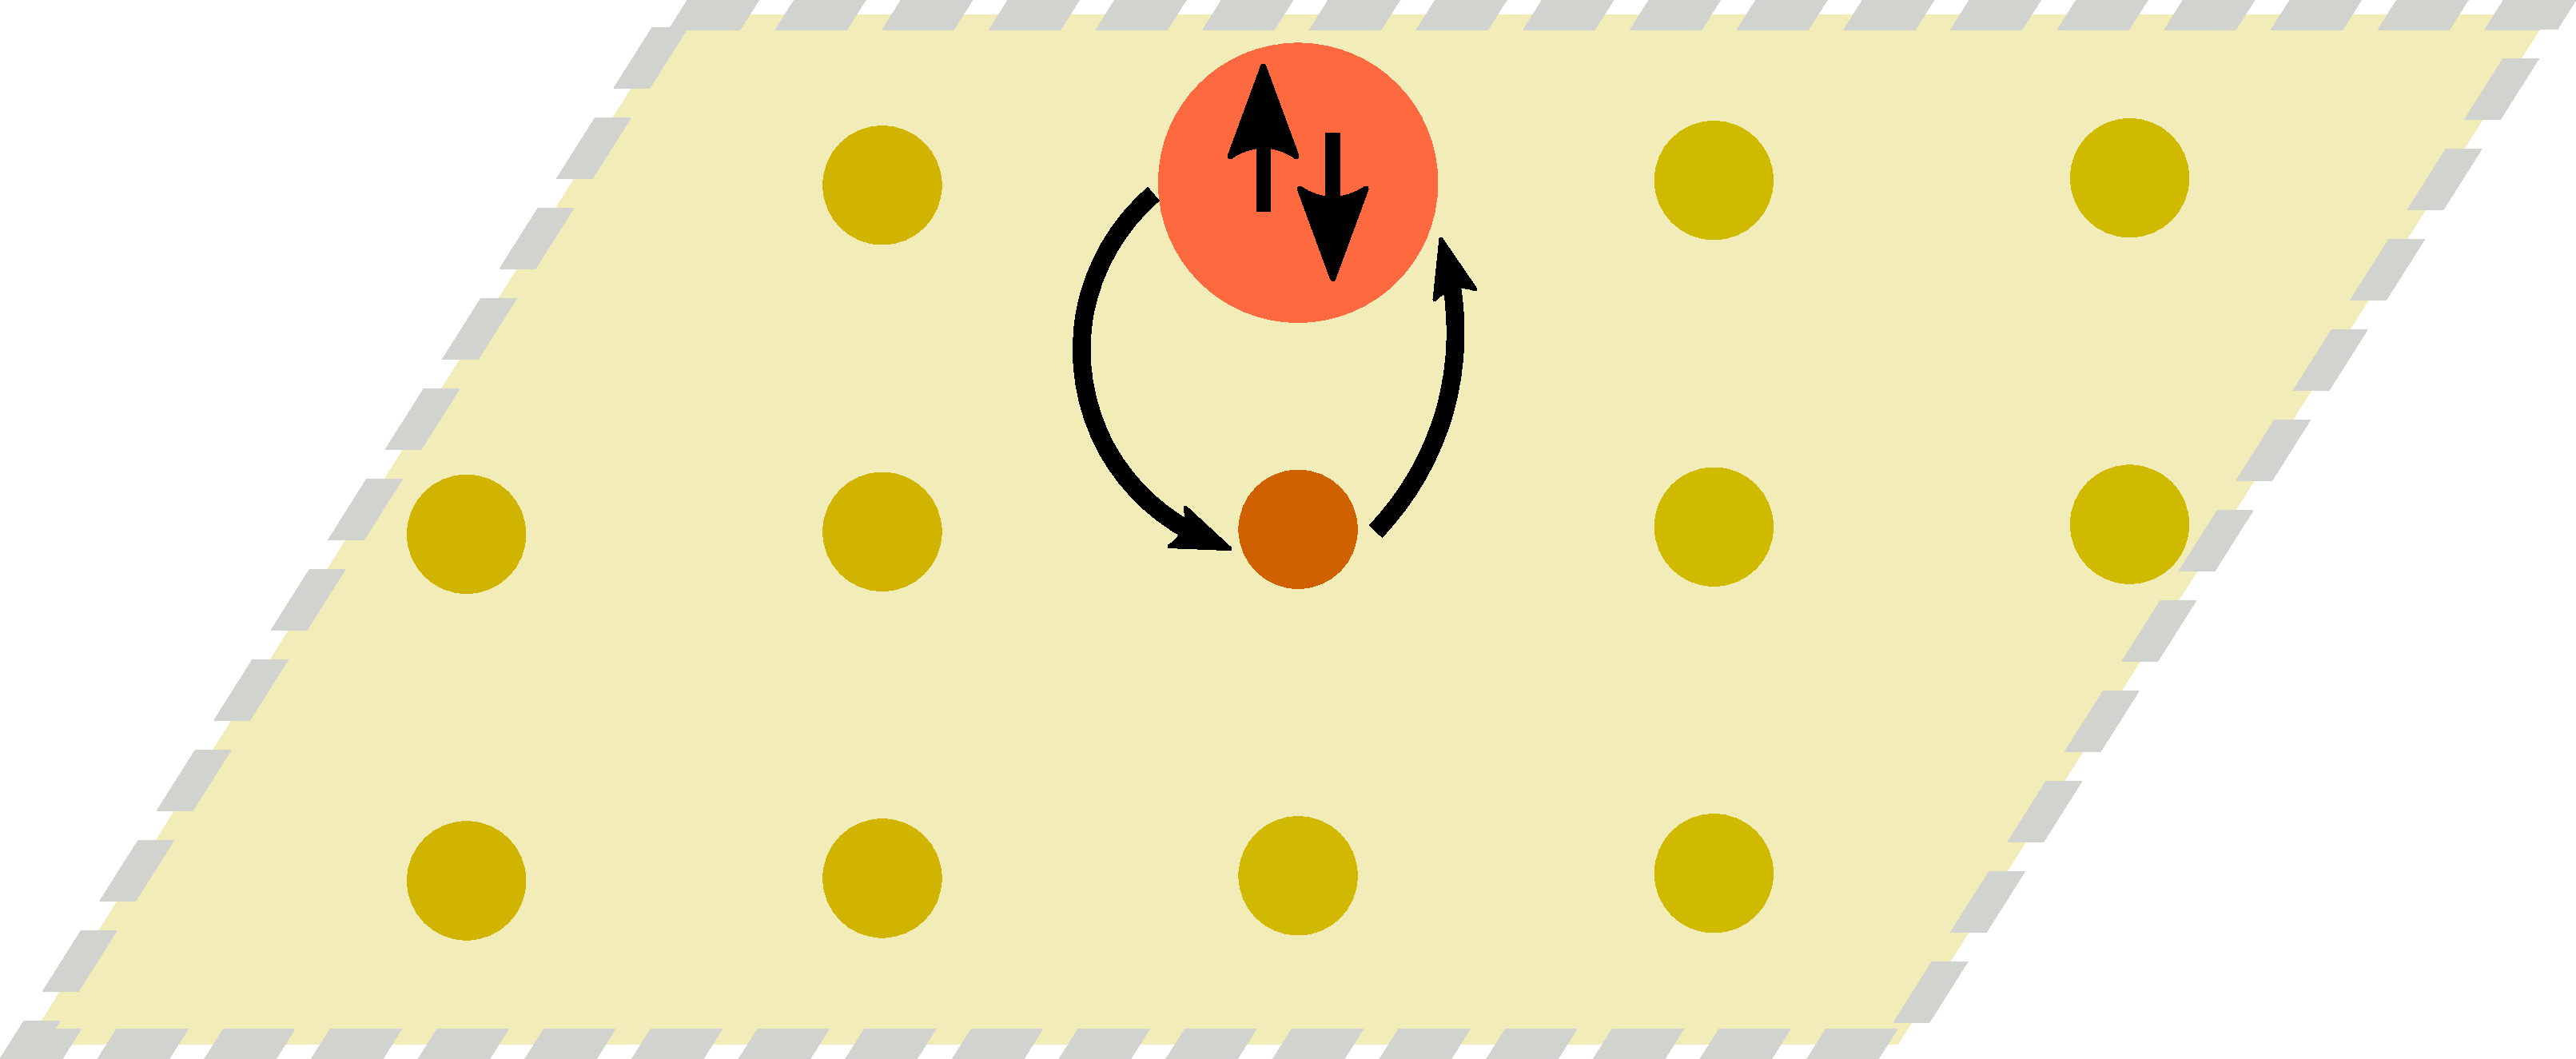
\includegraphics[width=\textwidth]{kondo-effect.pdf}
\end{minipage}
\end{frame}

\begin{frame}{Theory for the single-channel Kondo cloud}
\footcite{kondo1964resistance,wilson1975,andreiKondoreview,hewson1993,nozieres1974fermi,anderson1970,tsvelickKondoreview,affleck1993exact,Goldhaber-Gordon1998,Borzenets2020,sakai_osamu_shimizu,costi_hewson_1990,nozaki2012,affleck1995conformal}

\begin{minipage}{0.49\textwidth}
\centering
\begin{itemize}
\nitem spectral function \& magnetic susceptibility
\end{itemize}

\vspace*{10pt}

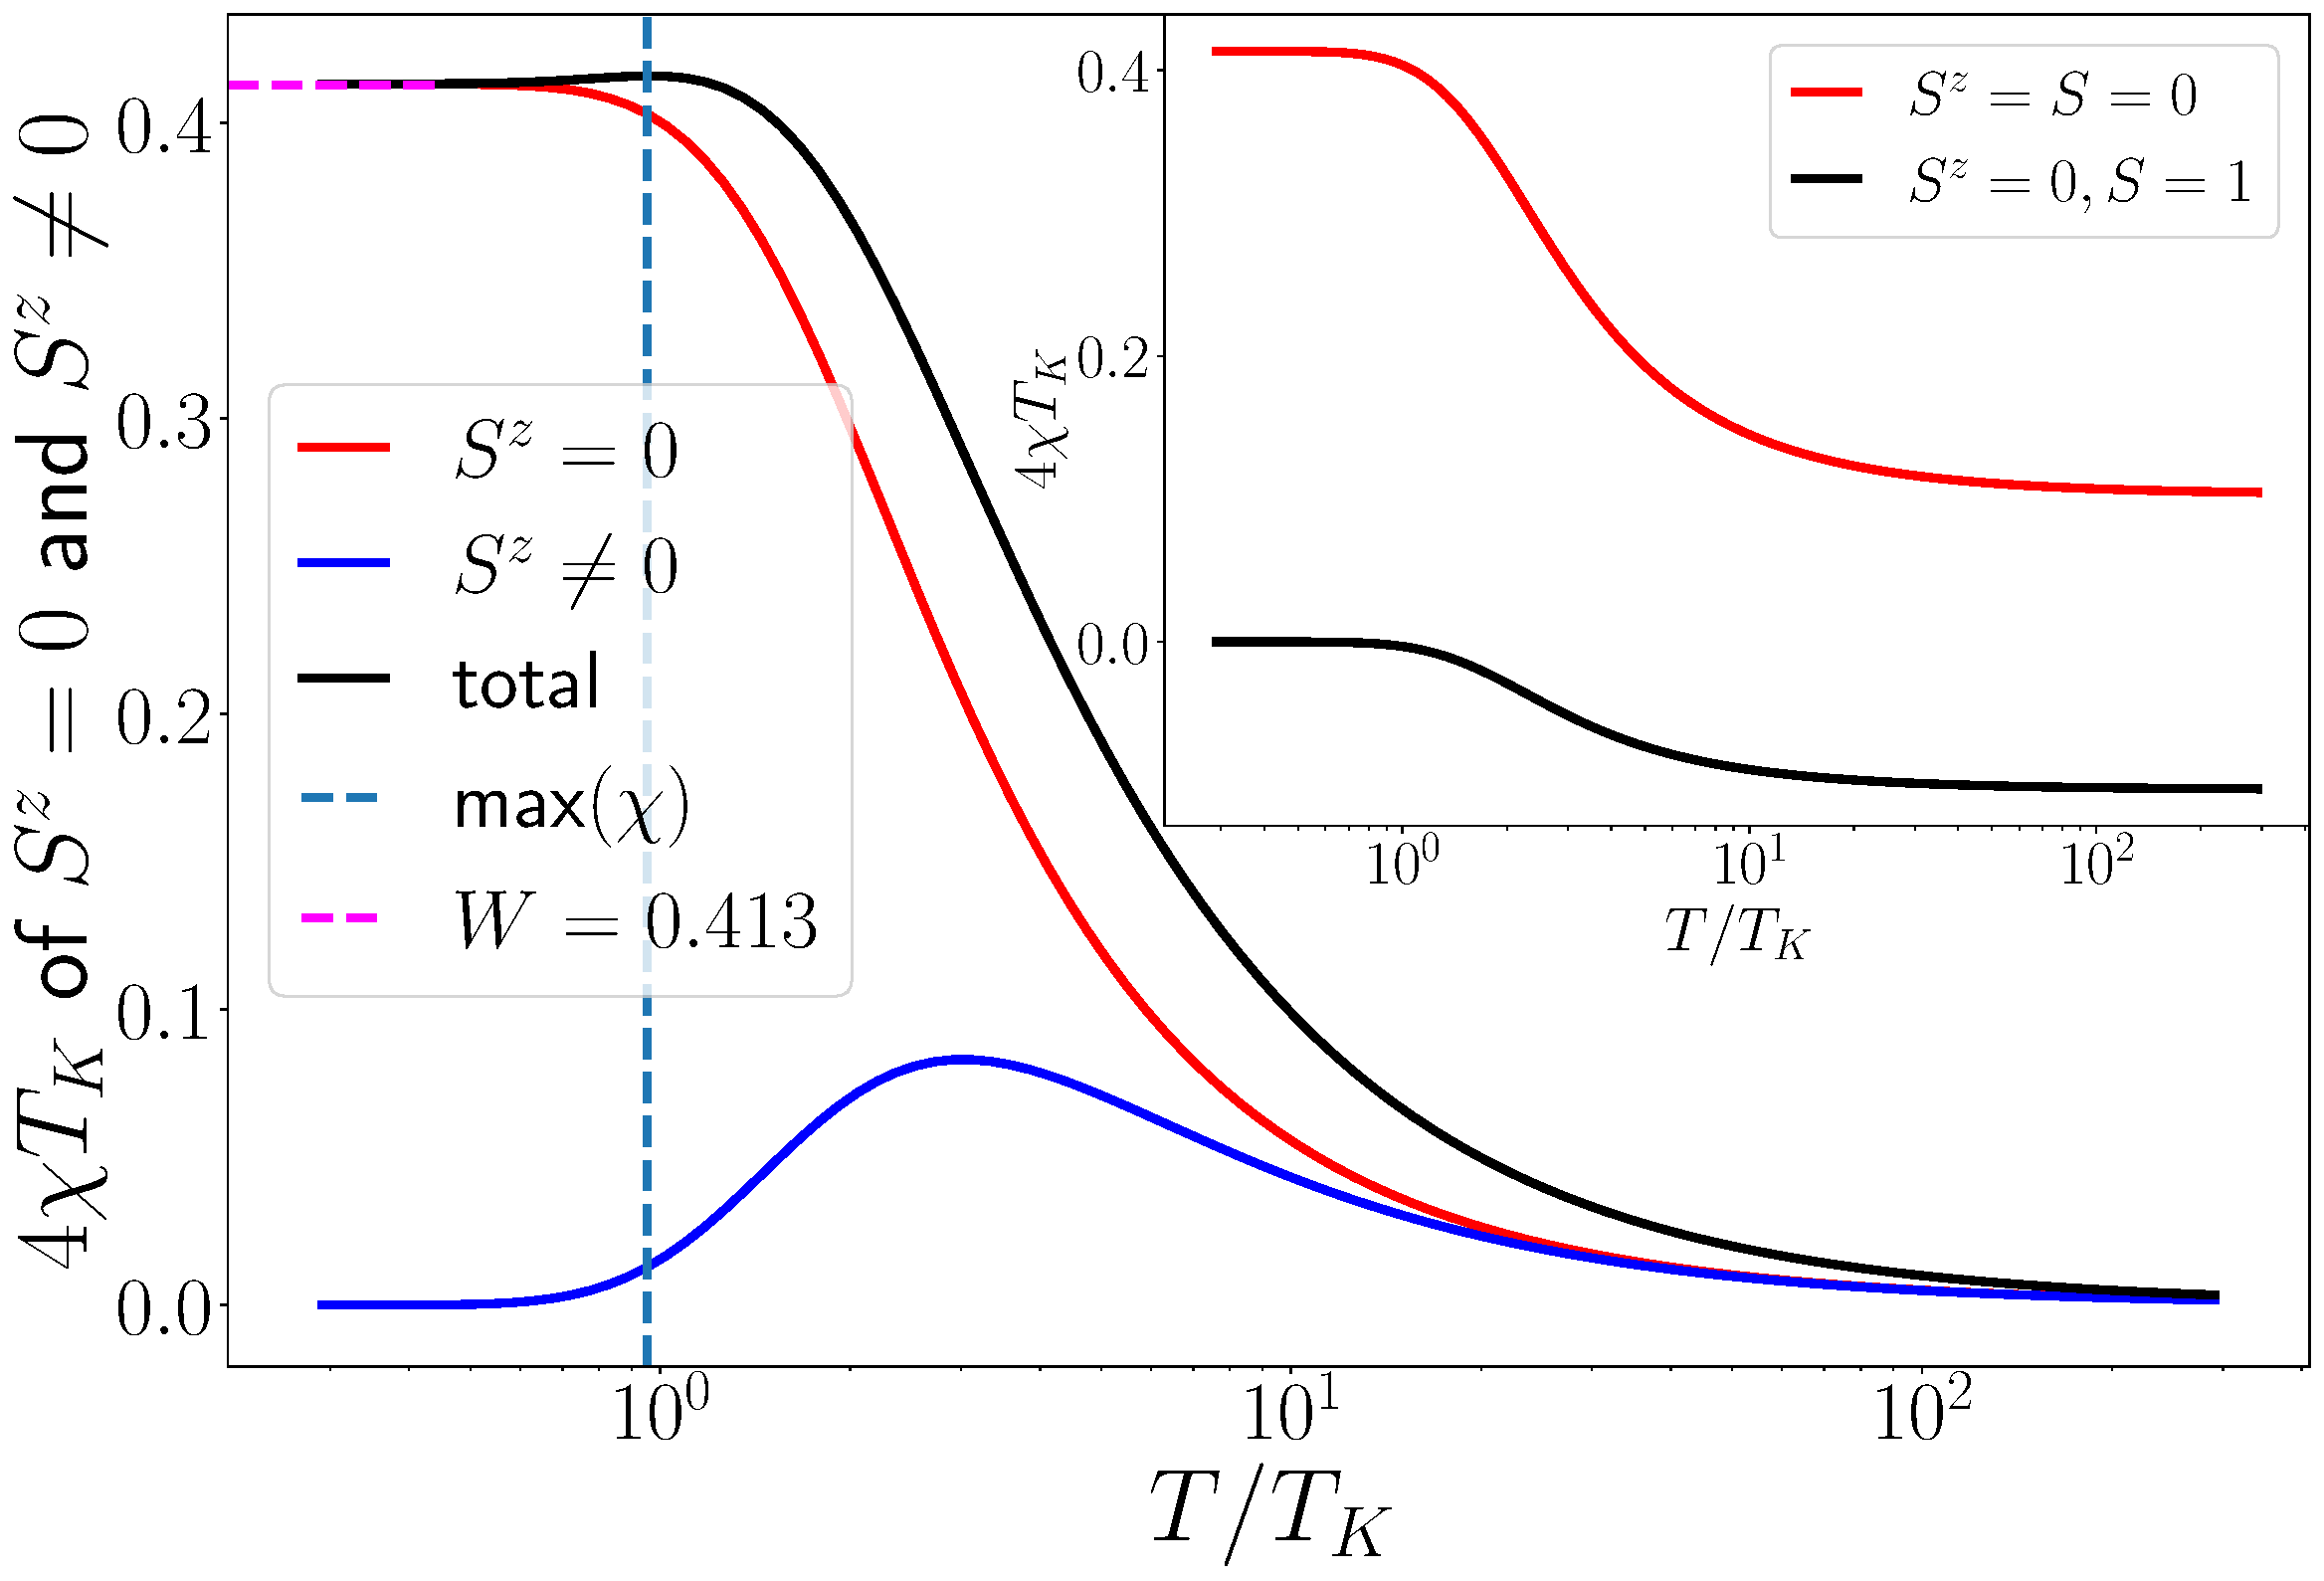
\includegraphics[width=0.8\textwidth]{chi_parts.pdf}
\end{minipage}
\begin{minipage}{0.49\textwidth}
\centering
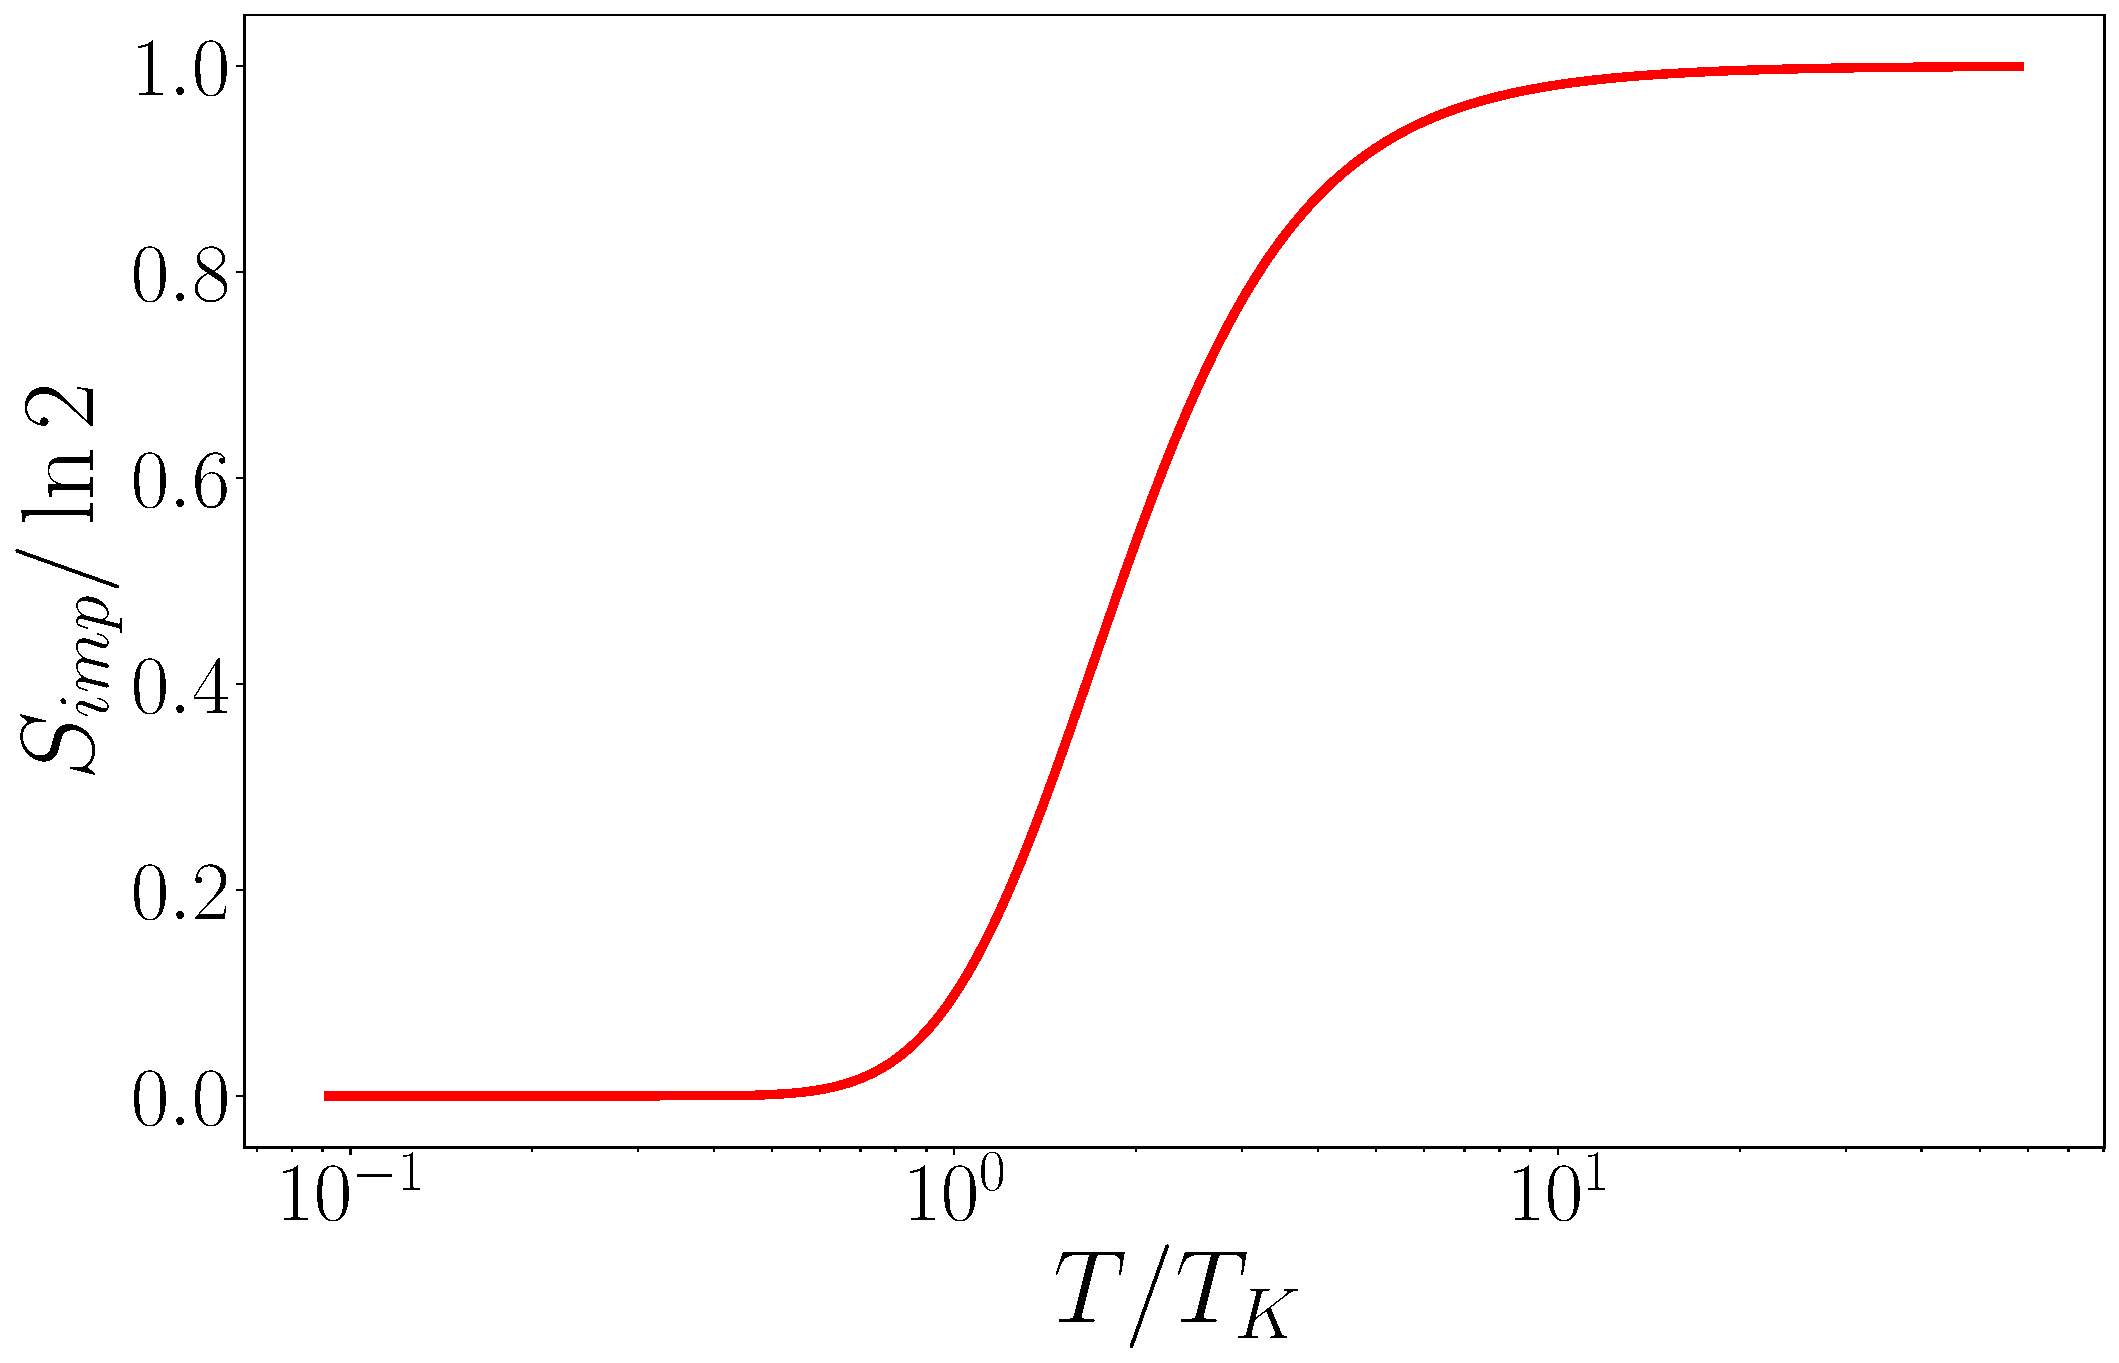
\includegraphics[width=0.8\textwidth]{entropy_therm.pdf}

\vspace*{10pt}

\begin{itemize}
\nitem local Fermi liq. \& orthogonality catastrophe
\nitem thermal entropy
\end{itemize}
\end{minipage}

\end{frame}

\begin{frame}{}
\section{Role of degeneracy in the multi-channel Kondo problem}
\begin{minipage}{0.55\textwidth}
	\small{{\bf arXiv:2205.00790}\\[10pt]
Siddhartha Patra, \alert{Abhirup Mukherjee}, Anirban Mukherjee, N. S. Vidhyadhiraja, A. Taraphder, Siddhartha Lal}
\end{minipage}
\hspace*{\fill}
\begin{minipage}{0.4\textwidth}
	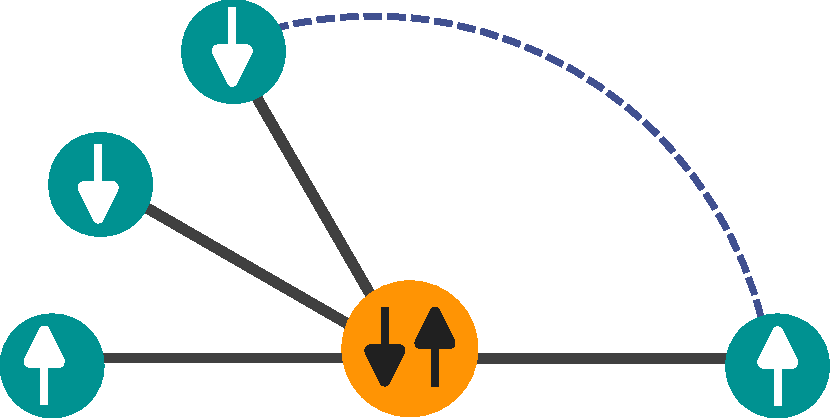
\includegraphics[width=\textwidth]{stargraph.pdf}
\end{minipage}
\end{frame}

\begin{frame}{Role of degeneracy in the multi-channel Kondo problem}
\footcite{Noz_blandin_1980,Tsvelick_weigmann_mchannel_1985,affleck1993exact,Gan_mchannel_1994,affleck_1991_overscreen,emery_kivelson,bulla_1998}

\begin{enumerate}
	\only<1>{\nitem Intermediate-coupling RG fixed point Hamiltonian and \alert{degenerate} ground states
	\nitem Degree of compensation, magnetization and susceptibility show \alert{incomplete screening}}
	\only<2>{\nitem Local \alert{marginal Fermi liquid} within the low-energy excitations of the bath
\nitem \alert{Duality} relations constrain the RG flows of the MCK model}
\end{enumerate}
\vspace*{\fill}

\only<1>{
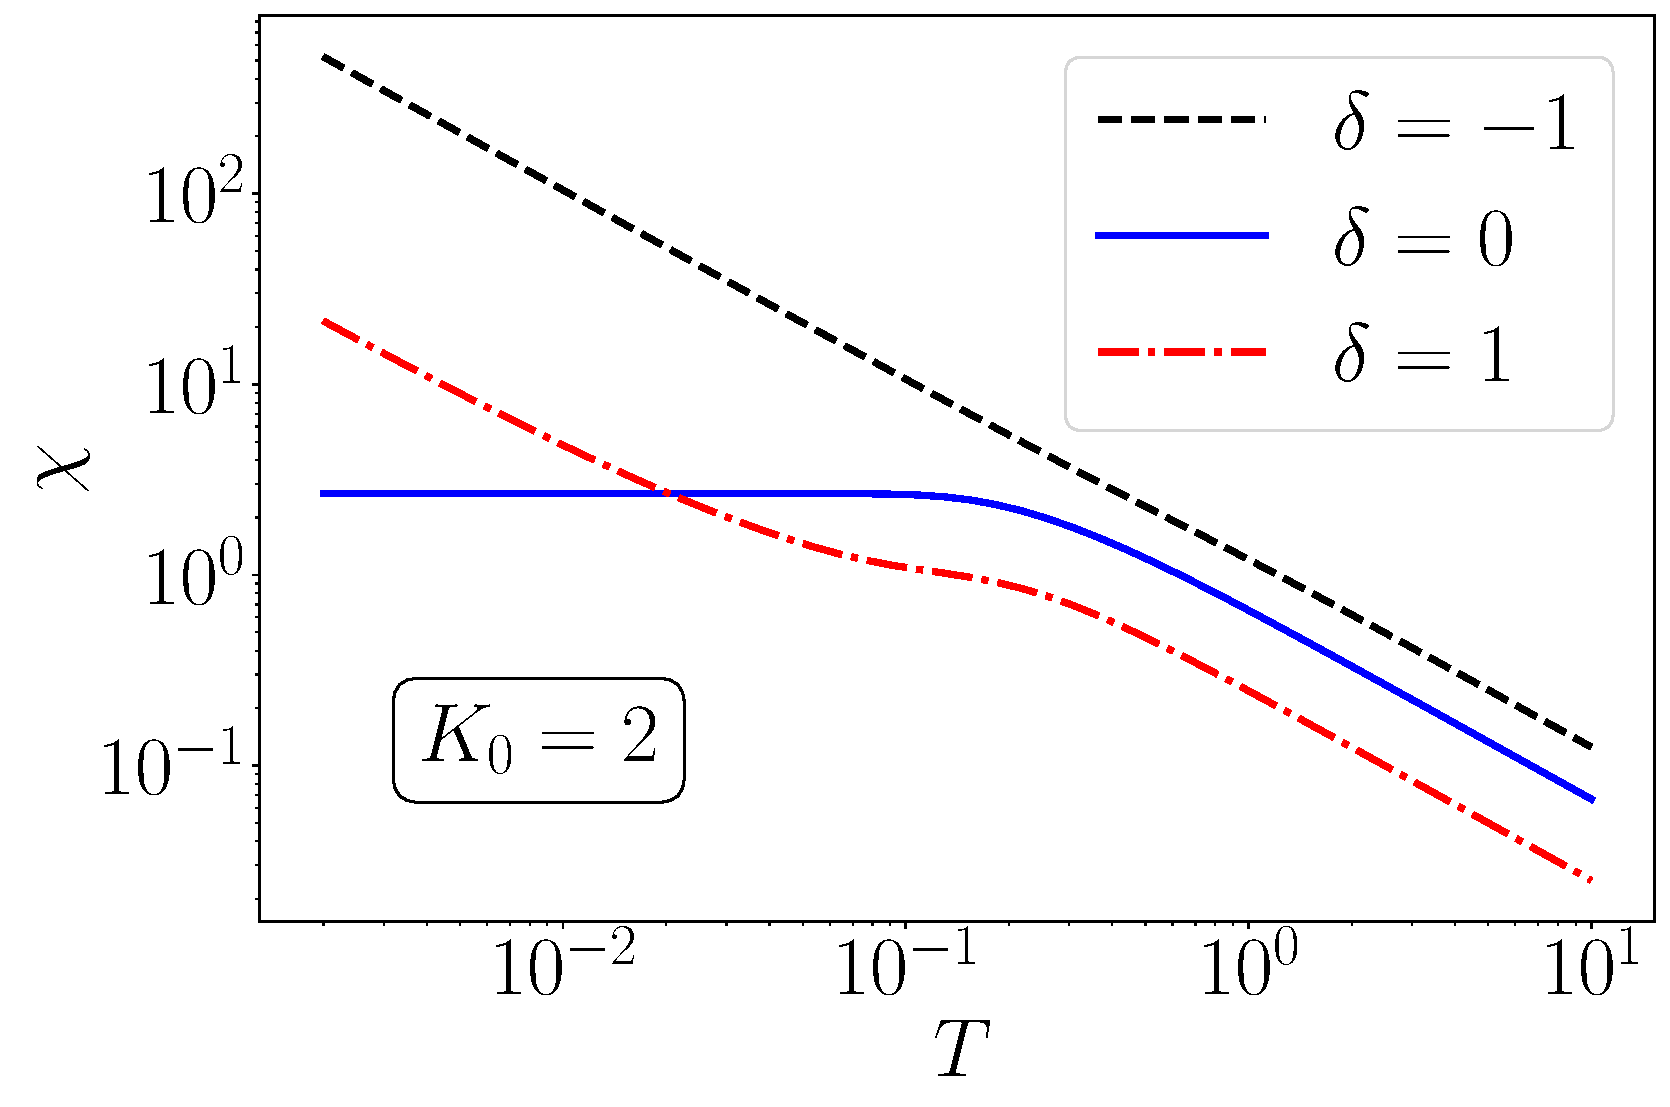
\includegraphics[width=0.4\textwidth]{CentralFieldChiPowerlaw.pdf}
\hspace*{\fill}
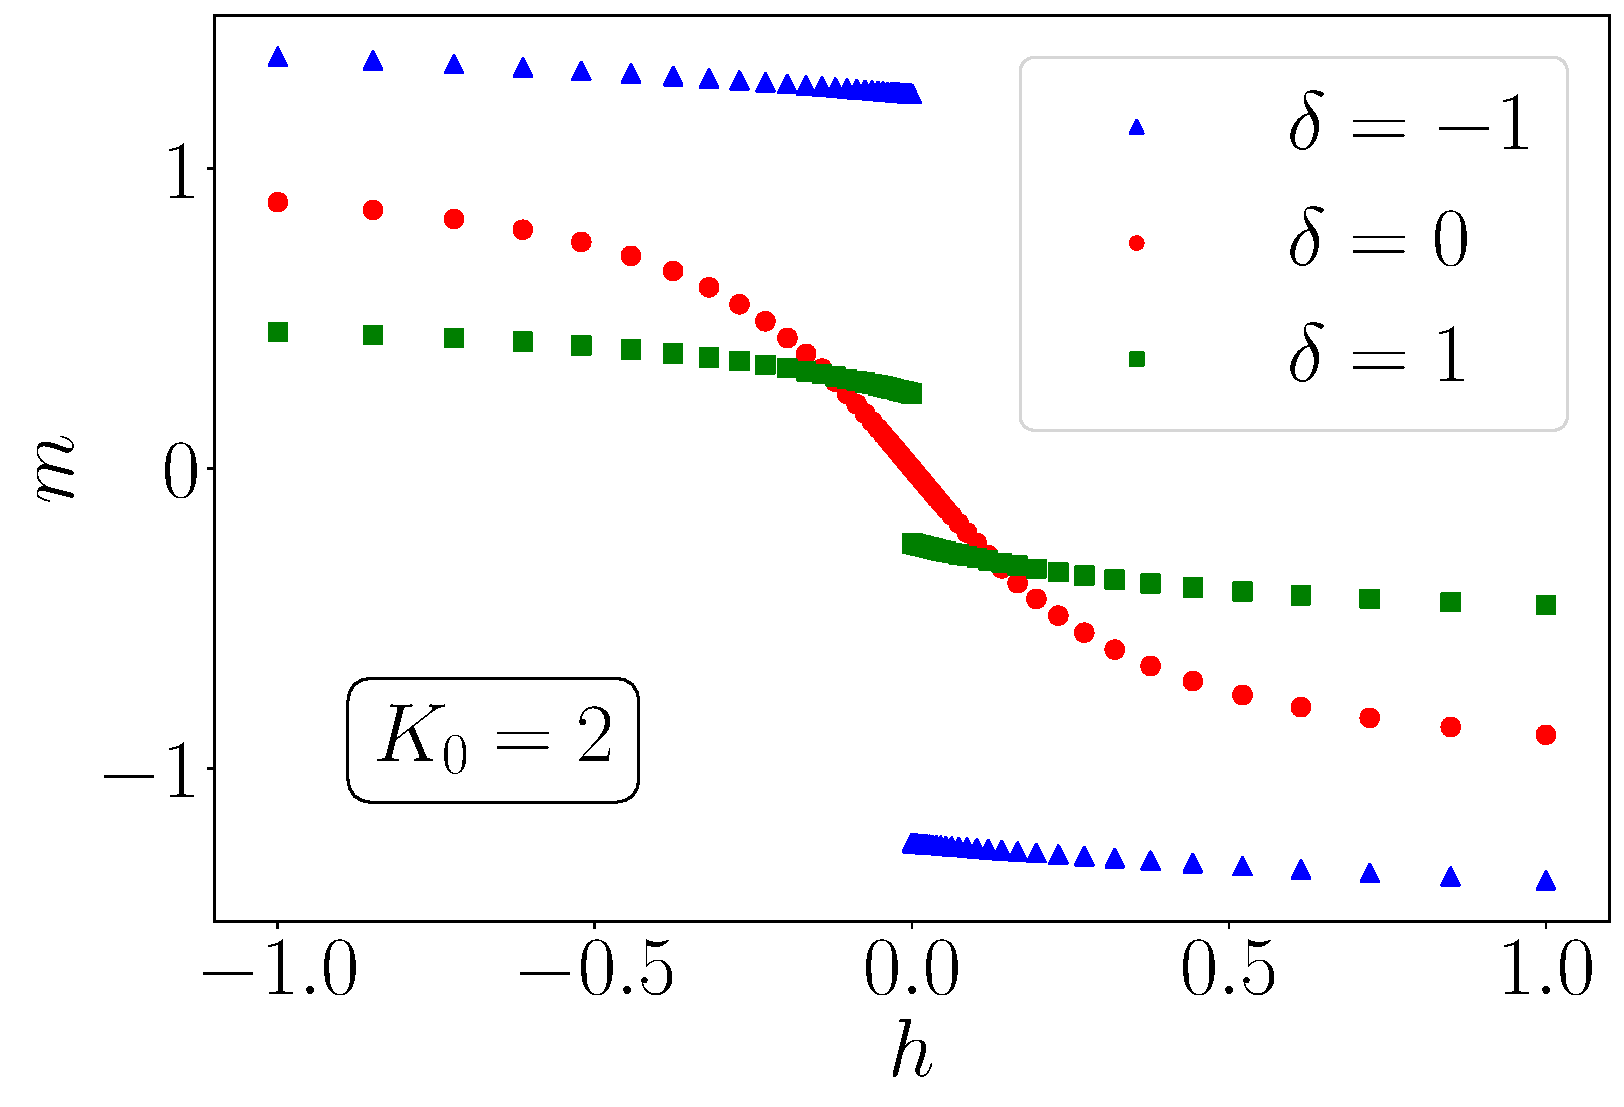
\includegraphics[width=0.4\textwidth]{discmagimpgen.pdf}
}

\only<2>{
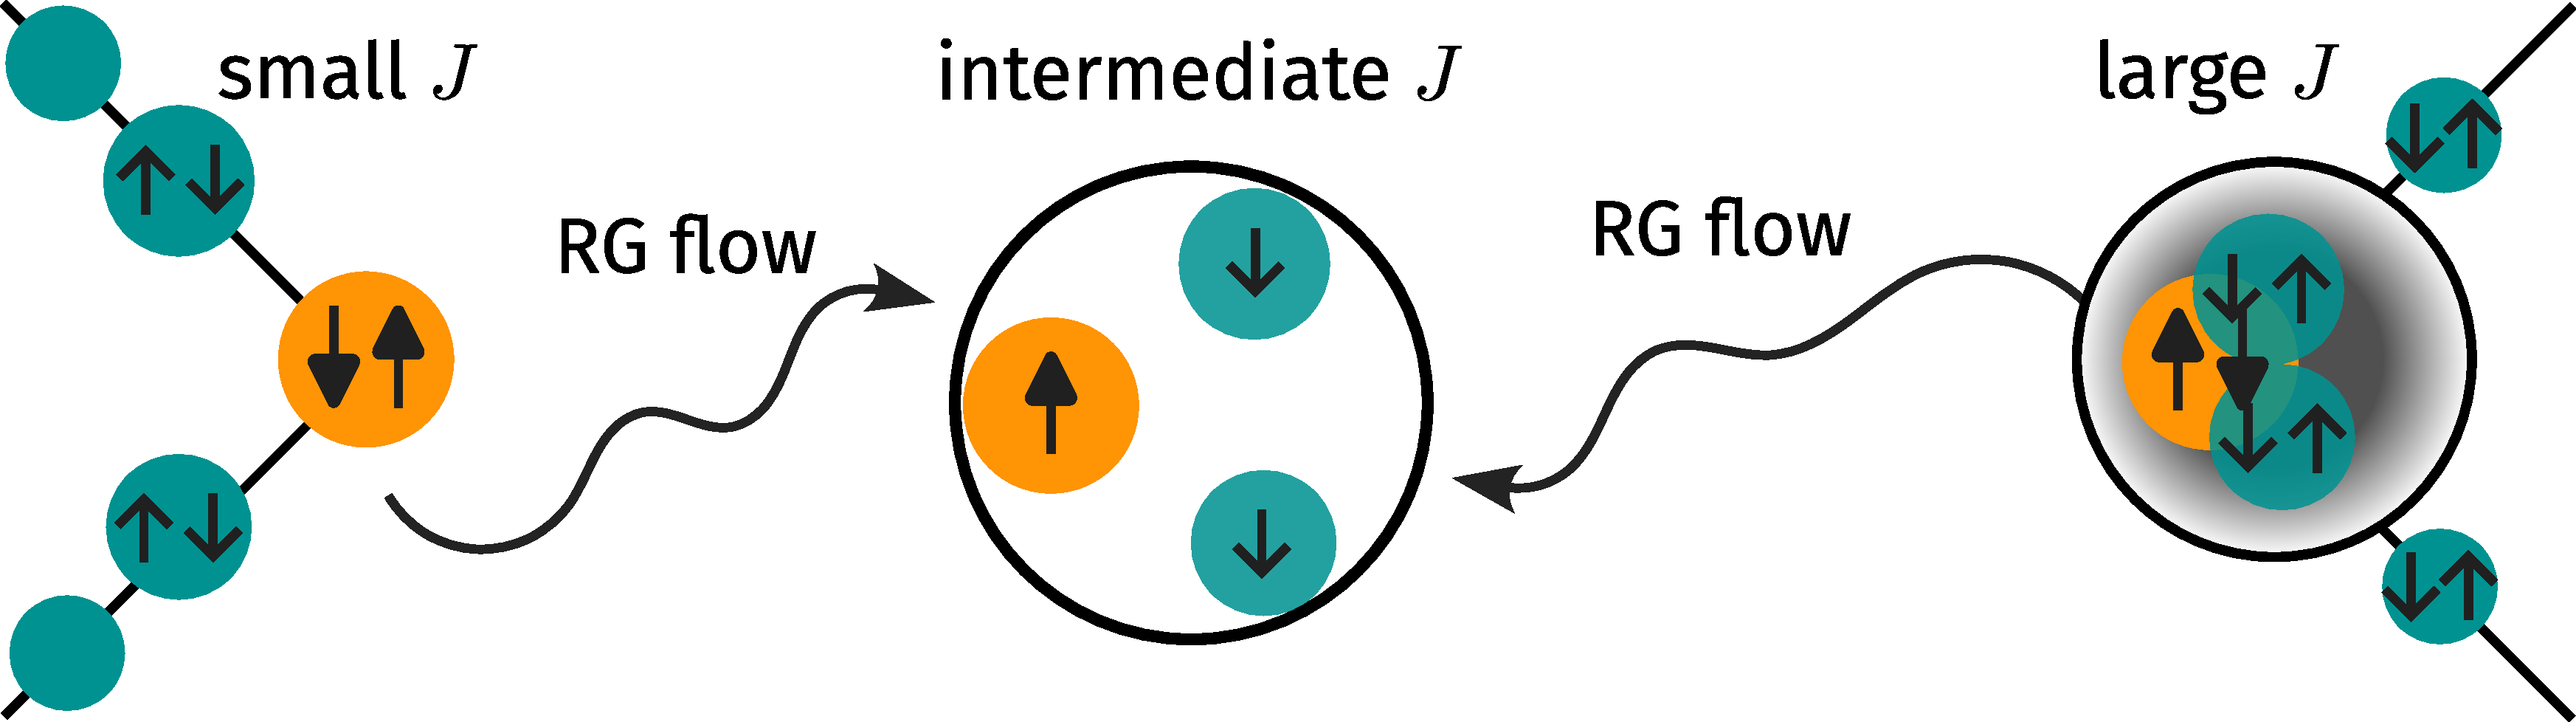
\includegraphics[width=0.7\textwidth]{duality.pdf}
}

\end{frame}

\begin{frame}{RG Phase diagram: }
\end{frame}

\begin{frame}{Local MIT in an extended Anderson impurity model}
\hspace*{-40pt}
\begin{minipage}{0.65\textwidth}
\begin{itemize}
\nitem Competition between $J$ and $U_b$ leads to phase transition from screened singlet phase at \(|U_b| \leq 4J\) to unscreened local moment phase at \(|U_b| > 4J\).
\nitem Impurity spectral function becomes gapped beyond the critical point.
\nitem Decoupling the impurity model leads to an effective model with the zeroth site as the correlated impurity, demonstrating the symmetry between the impurity and zeroth site.
\nitem Geometric entanglement and mutual information track the transition by vanishing beyond the critical point.
\nitem Subdominant pairing tendencies are observed near the quantum critical point.
\end{itemize}
\end{minipage}
\hspace*{5pt}
\begin{minipage}{0.41\textwidth}
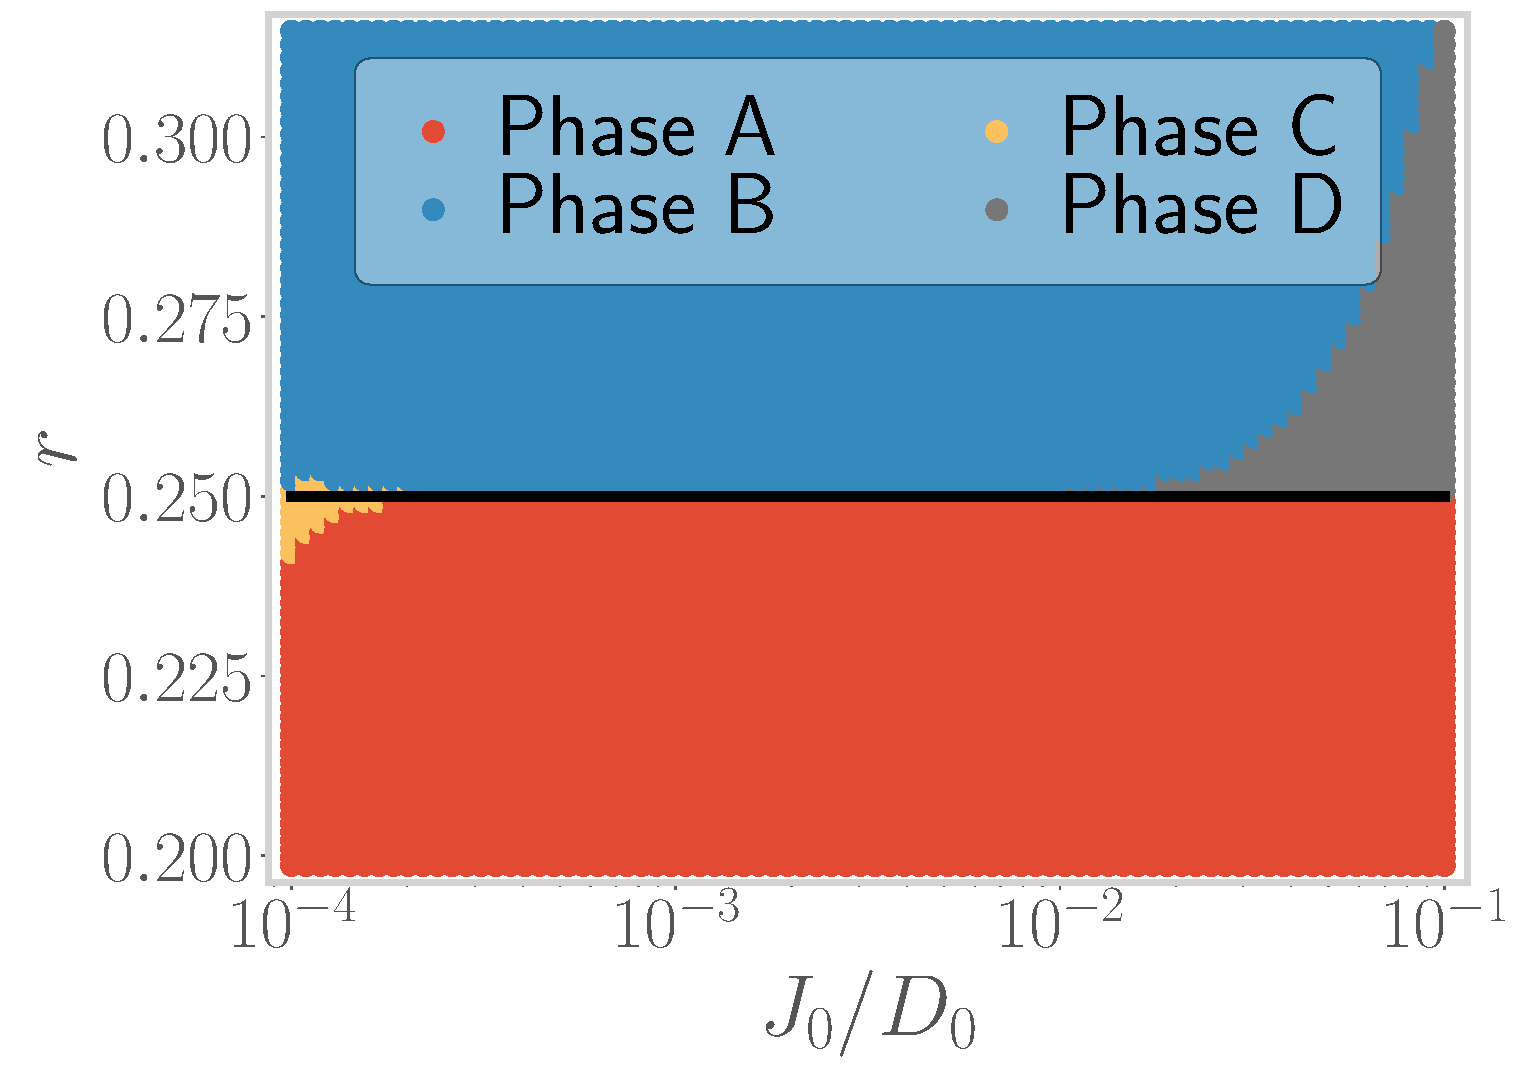
\includegraphics[width=0.9\textwidth]{phase-map-MIT.pdf}
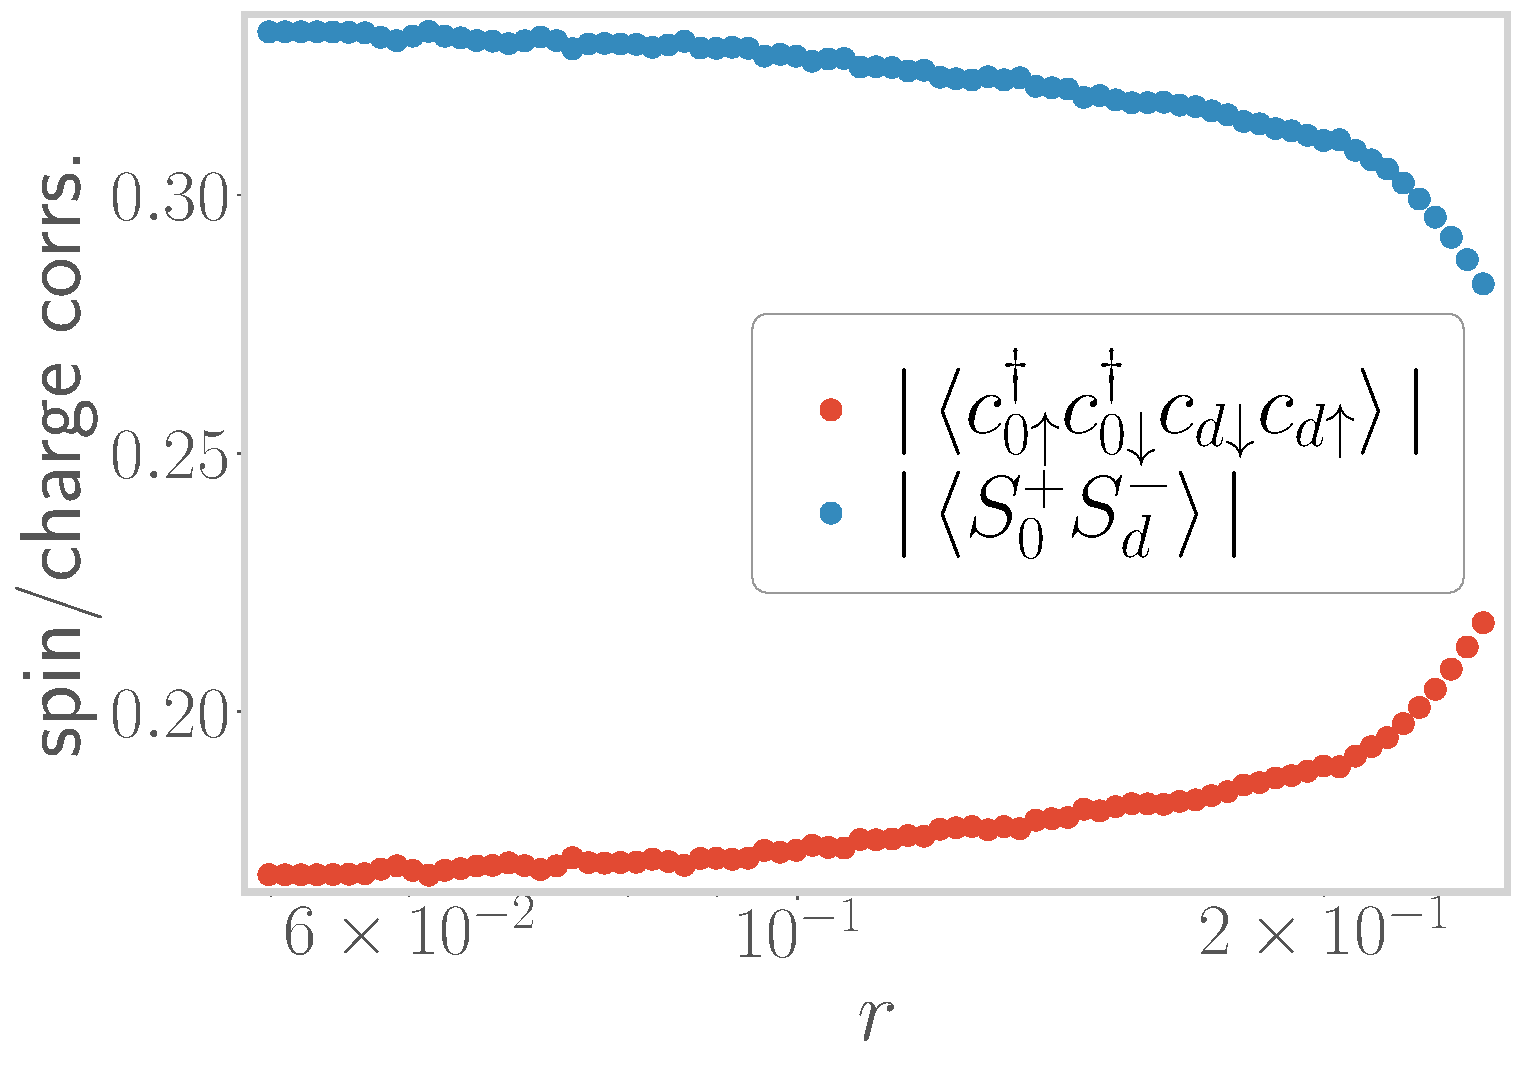
\includegraphics[width=0.9\textwidth]{odlro_d0.pdf}
\end{minipage}
\hspace*{-40pt}
\end{frame}

\begin{frame}{Presence of a phase transition}

\begin{minipage}{0.7\textwidth}
singlet {\LARGE \(\longrightarrow\)} spin+charge liquid {\LARGE \(\longrightarrow\)} local moment\\[10pt]
impurity spectral function gaps out
\end{minipage}
\begin{minipage}{0.29\textwidth}
\[r = -U_b/J\]
\[\ket{SS} = \ket{\uparrow,\downarrow} - \ket{\downarrow,\uparrow}\]
\[\ket{CT} = \ket{2,0} + \ket{0,2}\]
\end{minipage}

\vspace*{\fill}

\begin{minipage}{0.49\textwidth}
	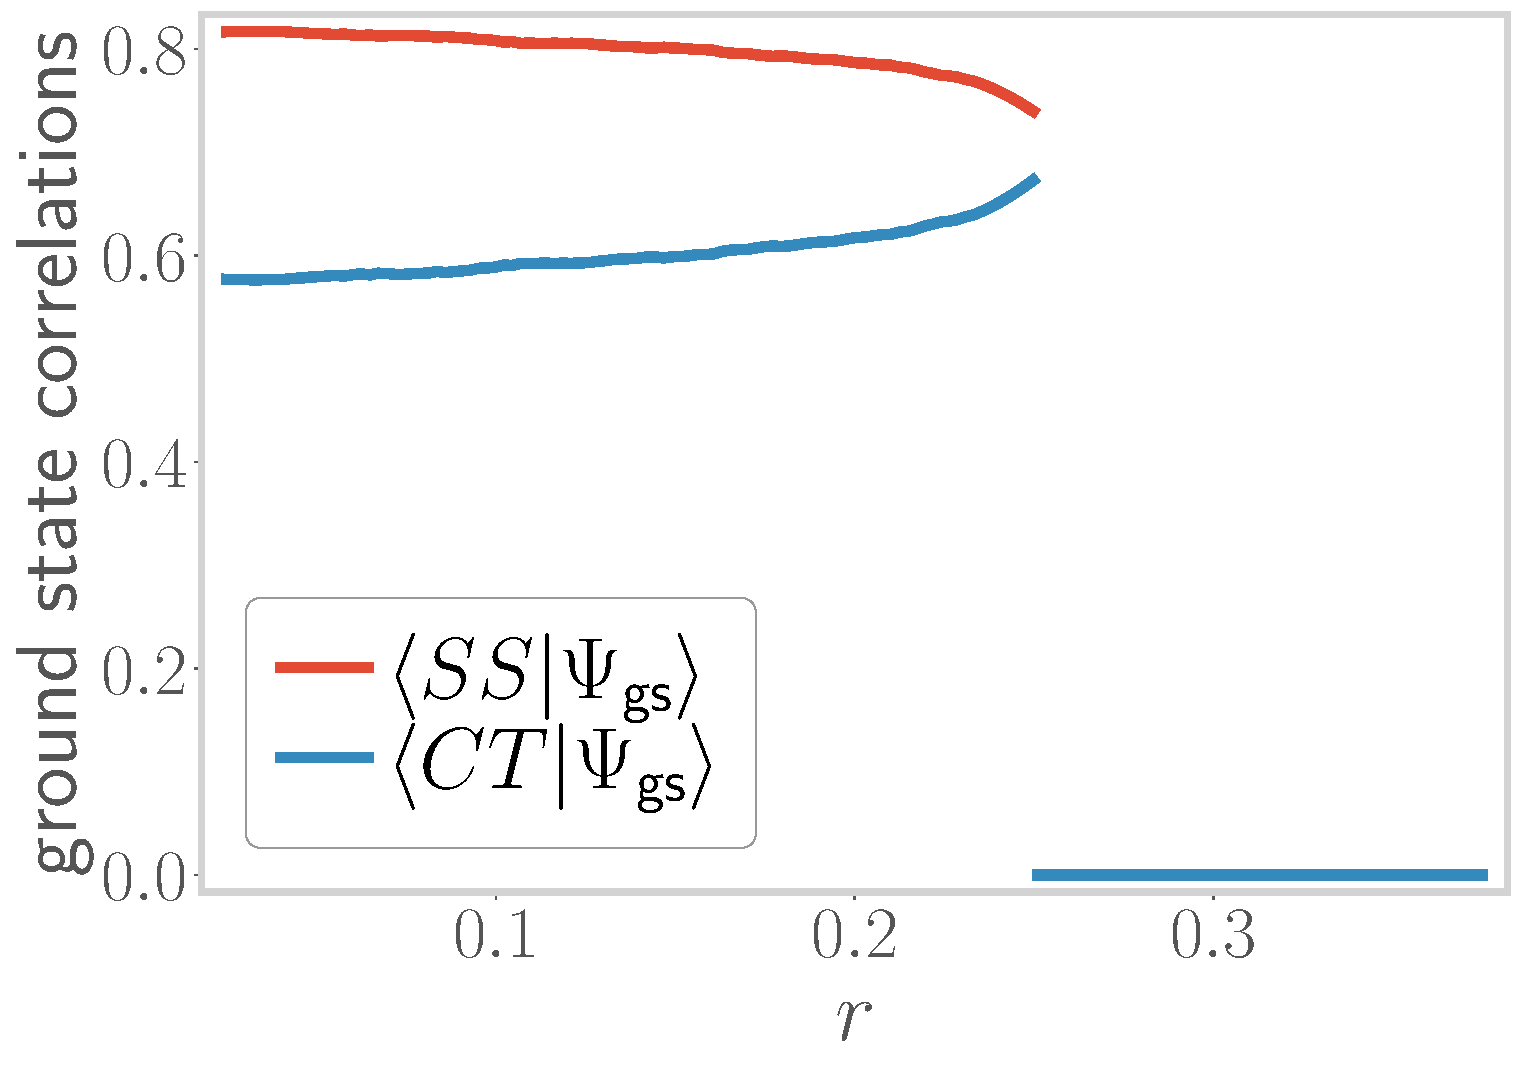
\includegraphics[width=\textwidth]{corrs_gs.pdf}
\end{minipage}
\hspace*{\fill}
\begin{minipage}{0.49\textwidth}
	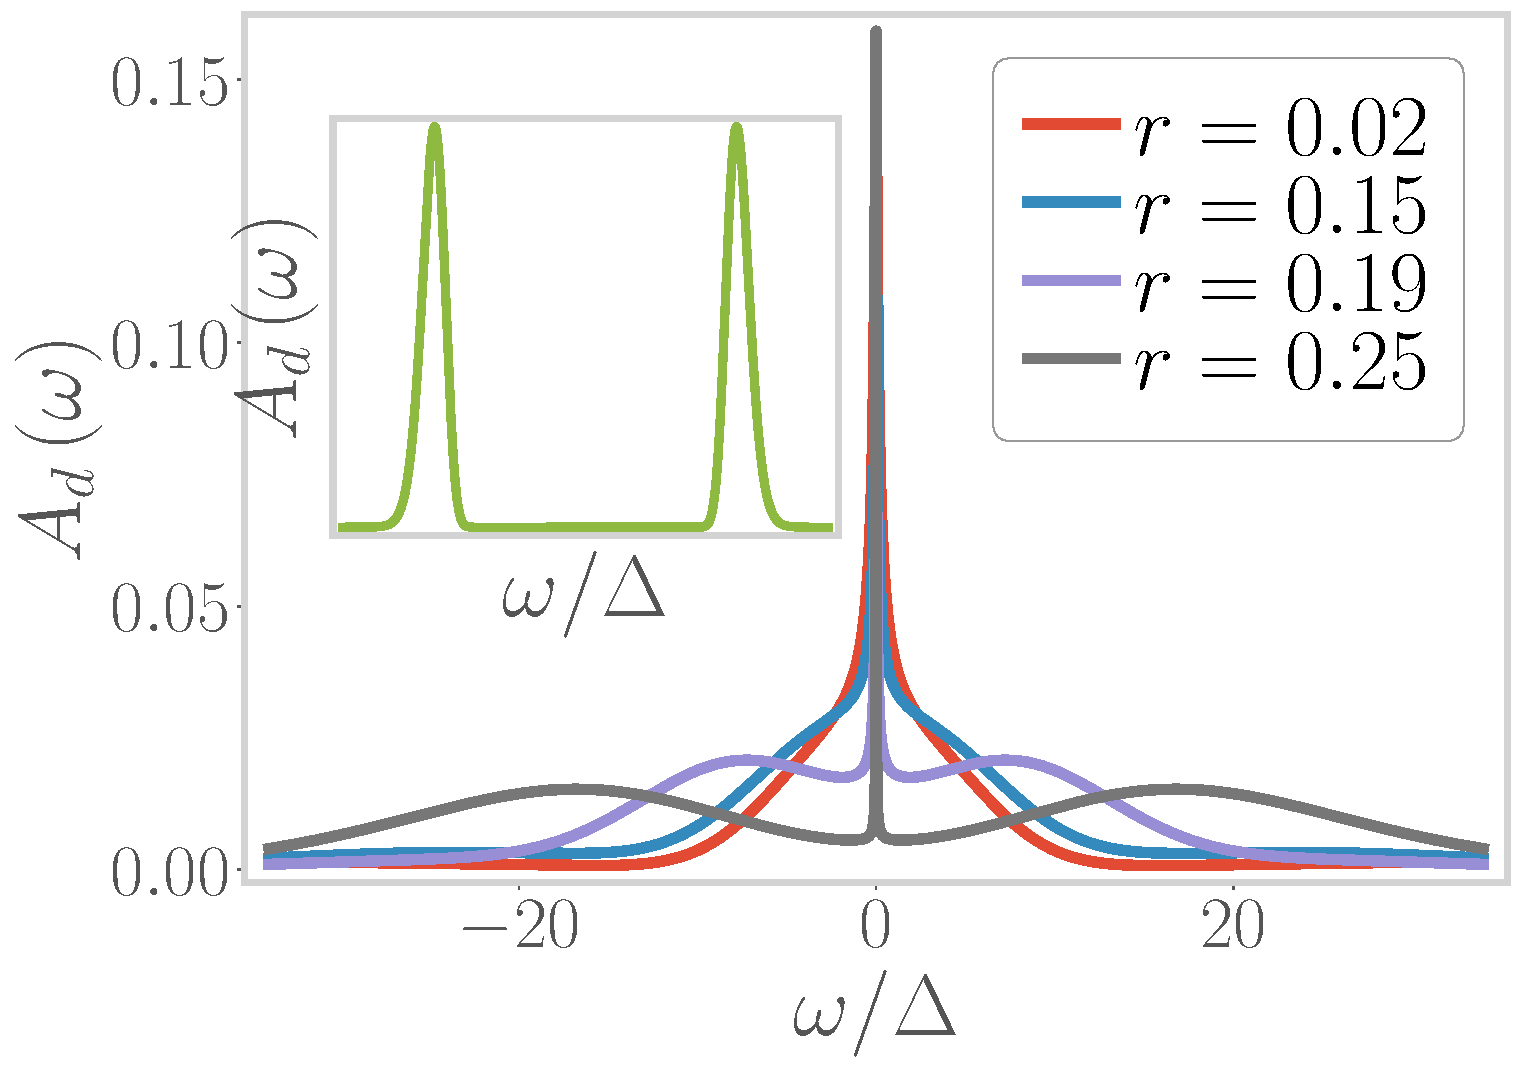
\includegraphics[width=\textwidth]{Add.pdf}
\end{minipage}
\end{frame}

\begin{frame}{Bath spectral function: towards self-consistency}
\begin{itemize}
\nitem Decoupling the impurity site leads  to an Anderson impurity model
	\[H_\text{0+rest} = \underbrace{-\left(U_0 + U_b\right)\left(\hat n_{0\uparrow} - \hat n_{0\downarrow}\right)^2}_\text{new correlated impurity} \underbrace{- t\sum_{j\in \text{n.n. of 0},\atop{\sigma}}\left(c^\dagger_{0\sigma}c_{j\sigma} + \text{h.c.}\right)}_\text{hopping between new impurity \& new bath} \underbrace{-t \sum_{\left<i,j \right>}\left(c^\dagger_{i\sigma}c_{j\sigma} + \text{h.c.}\right)}_\text{K.E. of new bath}\]\\[10pt]
\nitem correlated, dominant spin-flip processes lead to repulsive $U_\text{eff} = U_0 + U_b \sim J^*/8$\\[20pt]
\nitem \(J\) symmetrises the two sites, leading to similar spectral functions \(\longrightarrow\) essence of self-consistency
\end{itemize}
\end{frame}

\begin{frame}{Entanglement as a probe for the transition}

	Geometric entanglement: ~ \(\varepsilon(\psi_1,\psi_2) = 1 - |\braket{\psi_1|\psi_2}|^2\)\\[10pt]
	\(\longrightarrow \sqrt{1 -\varepsilon_\text{SS}}\sqrt{1 -\varepsilon_\text{CT}}\) is maximised, then vanishes\\[10pt]
	Mutual information between impurity and cloud vanishes\\[10pt]

\begin{minipage}{0.49\textwidth}
	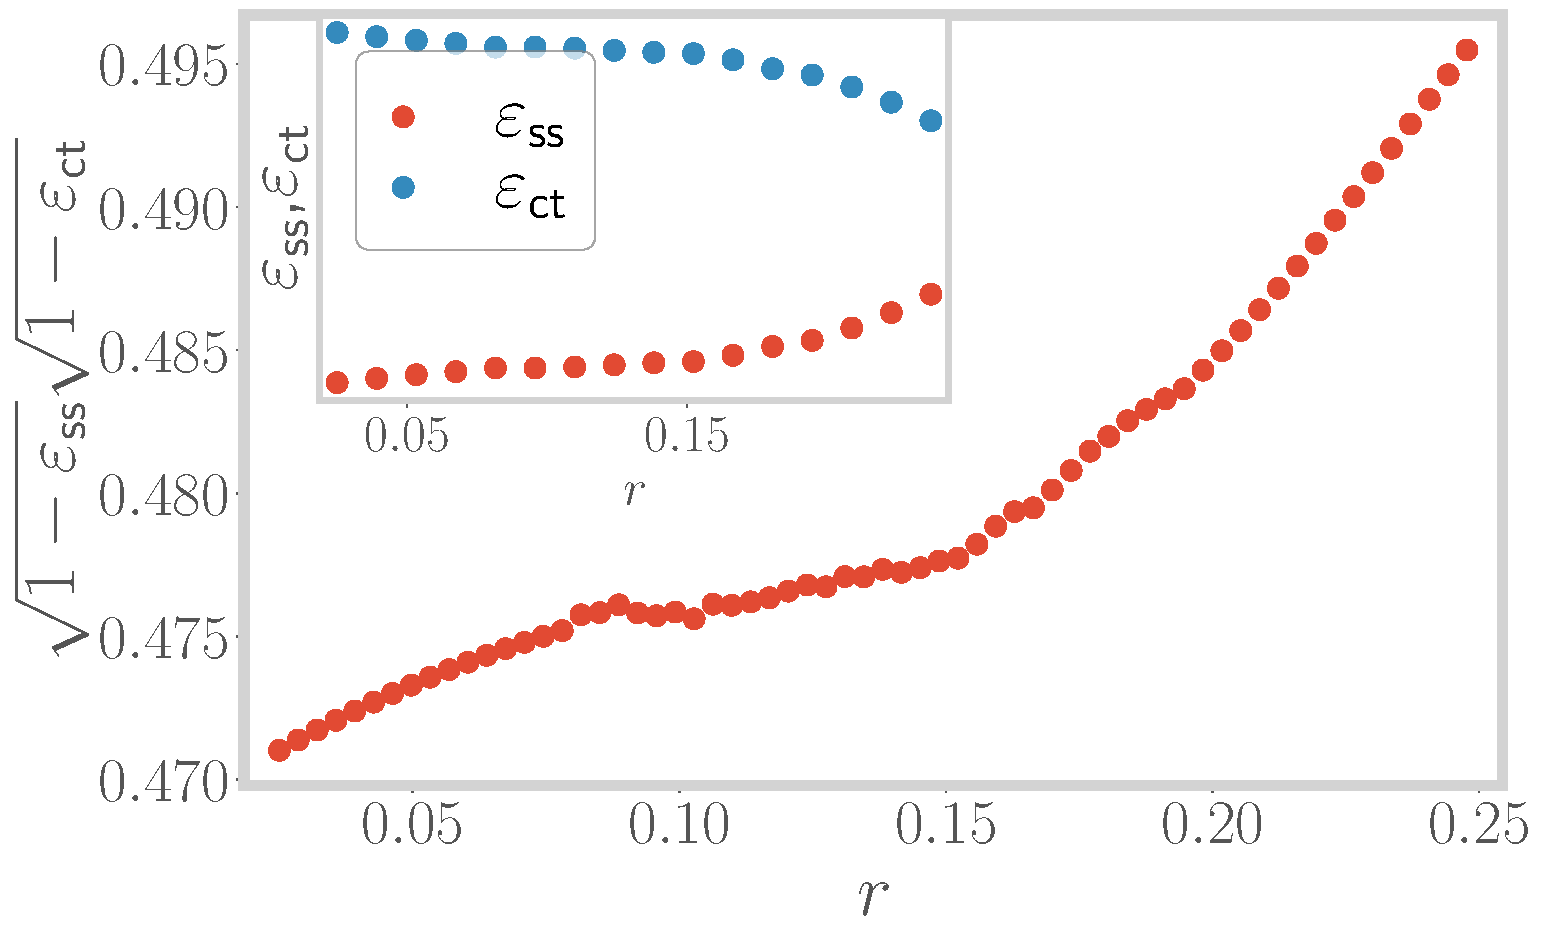
\includegraphics[width=\textwidth]{entanglement.pdf}
\end{minipage}
\hspace*{\fill}
\begin{minipage}{0.49\textwidth}
	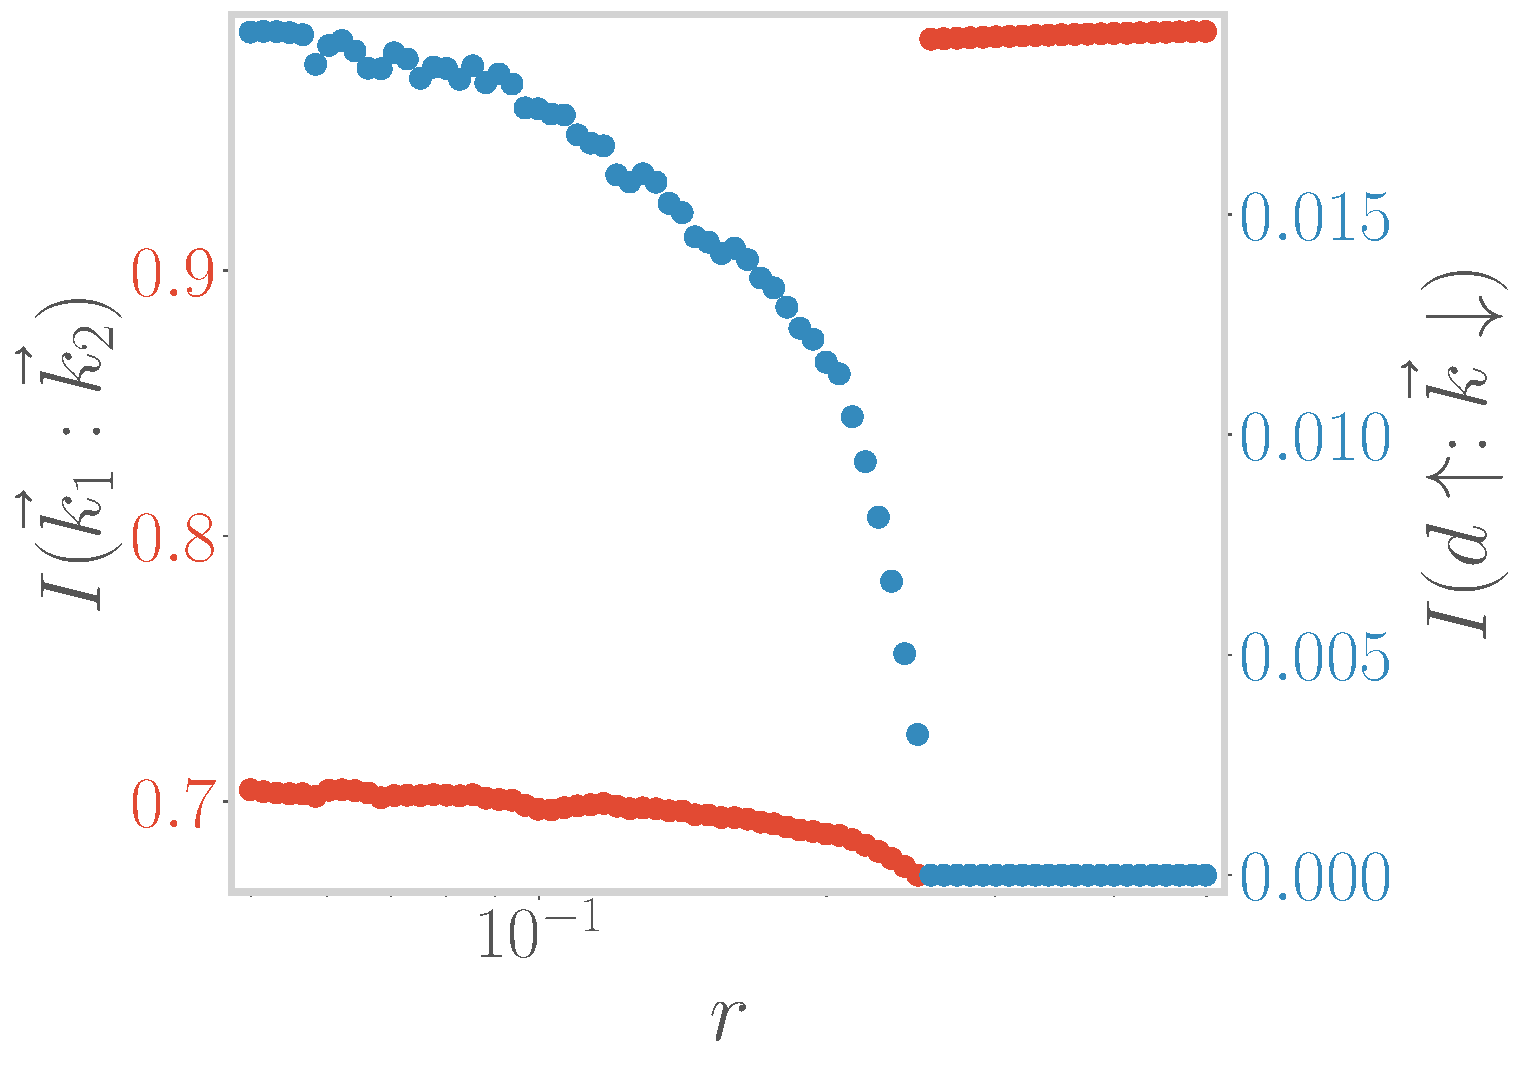
\includegraphics[width=\textwidth]{I_k.pdf}
\end{minipage}

\end{frame}

\begin{frame}{Presence of subdominant pair fluctuations}
	
\begin{itemize}
	\nitem \alert{pairing tendencies} observed near the quantum critical point\\[10pt]
	\nitem might lead to \alert{superconductivity} with doping\\[10pt]
	\nitem seen in cuprates, heavy-fermions materials, pnictides, etc\\[10pt]
\end{itemize}
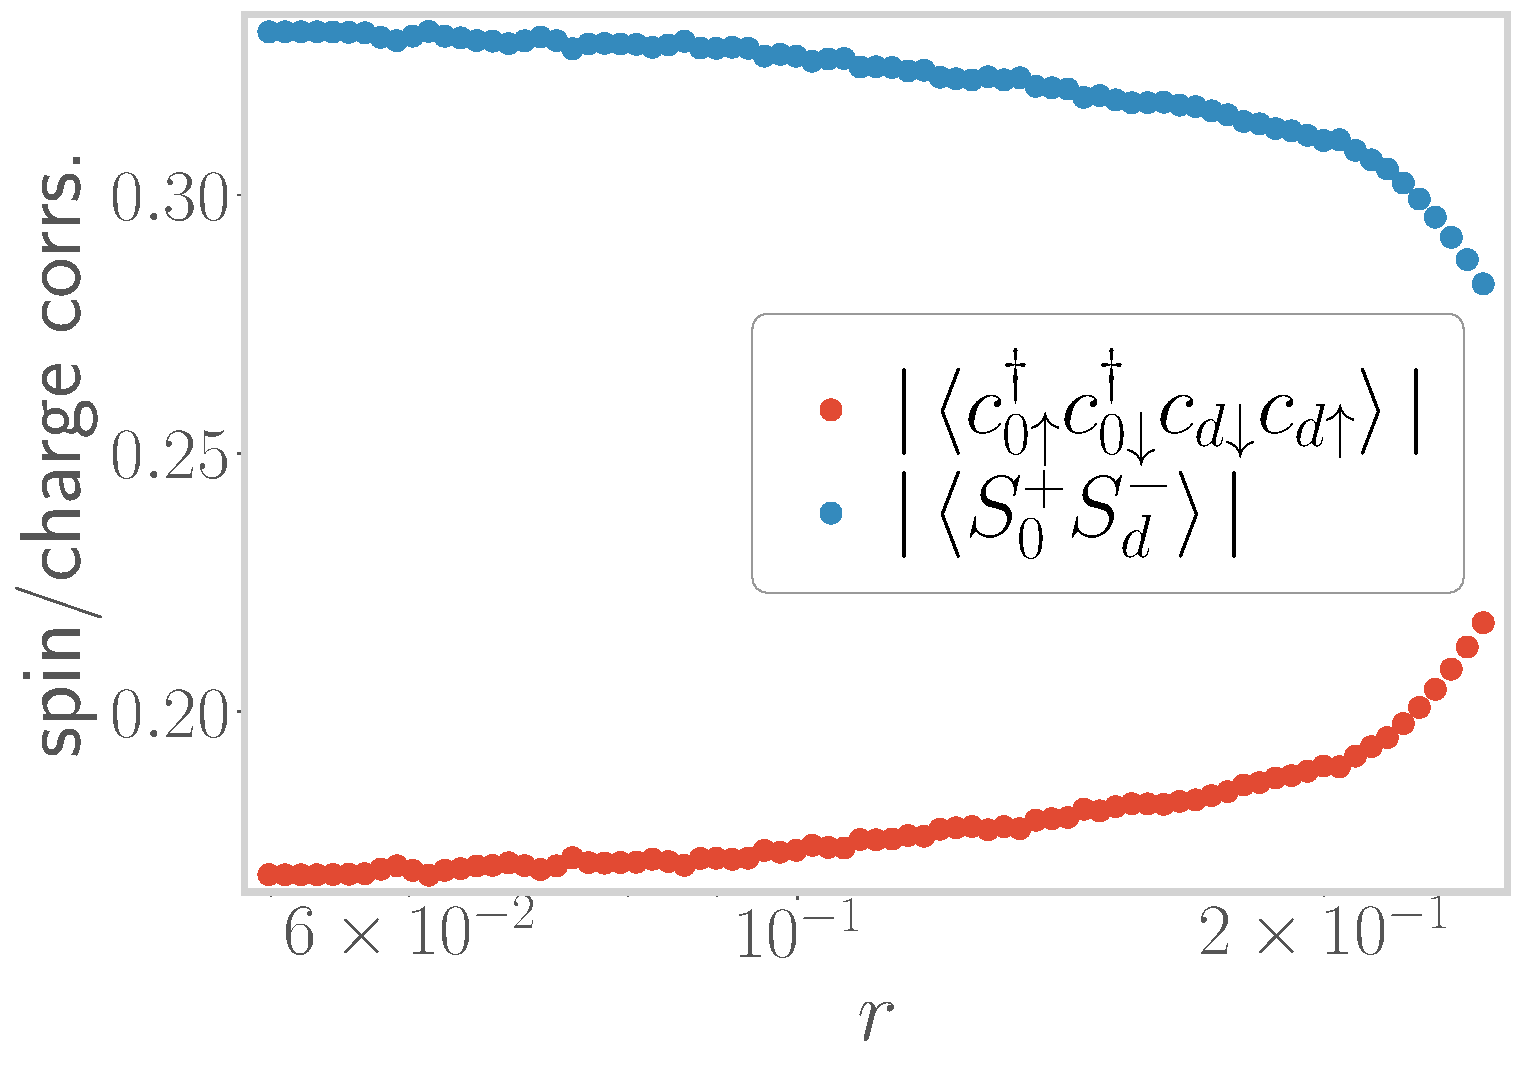
\includegraphics[width=0.45\textwidth]{odlro_d0.pdf}
\hspace*{\fill}
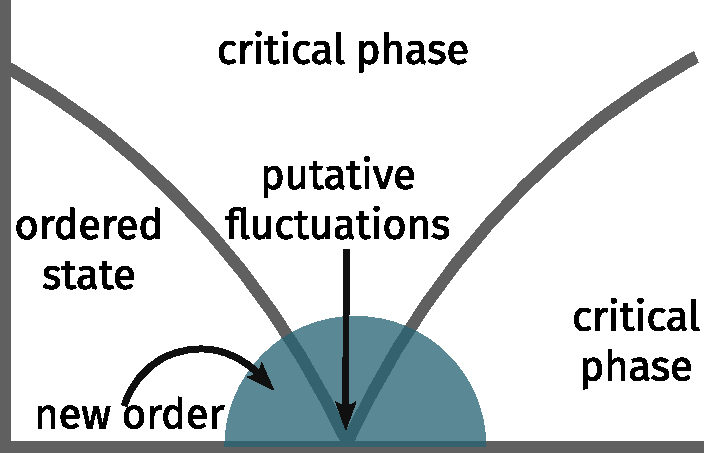
\includegraphics[width=0.45\textwidth]{gen-phase-diagram.pdf}
\end{frame}

\begin{frame}{}
\section{Entanglement scaling in free fermions: holography \& topology}

\begin{minipage}{0.3\textwidth}
	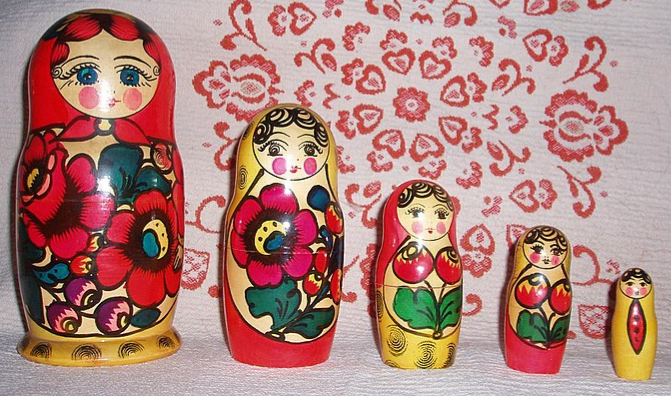
\includegraphics[width=\textwidth]{figures/Matroshka.png}
\end{minipage}
\hspace*{\fill}
\begin{minipage}{0.5\textwidth}
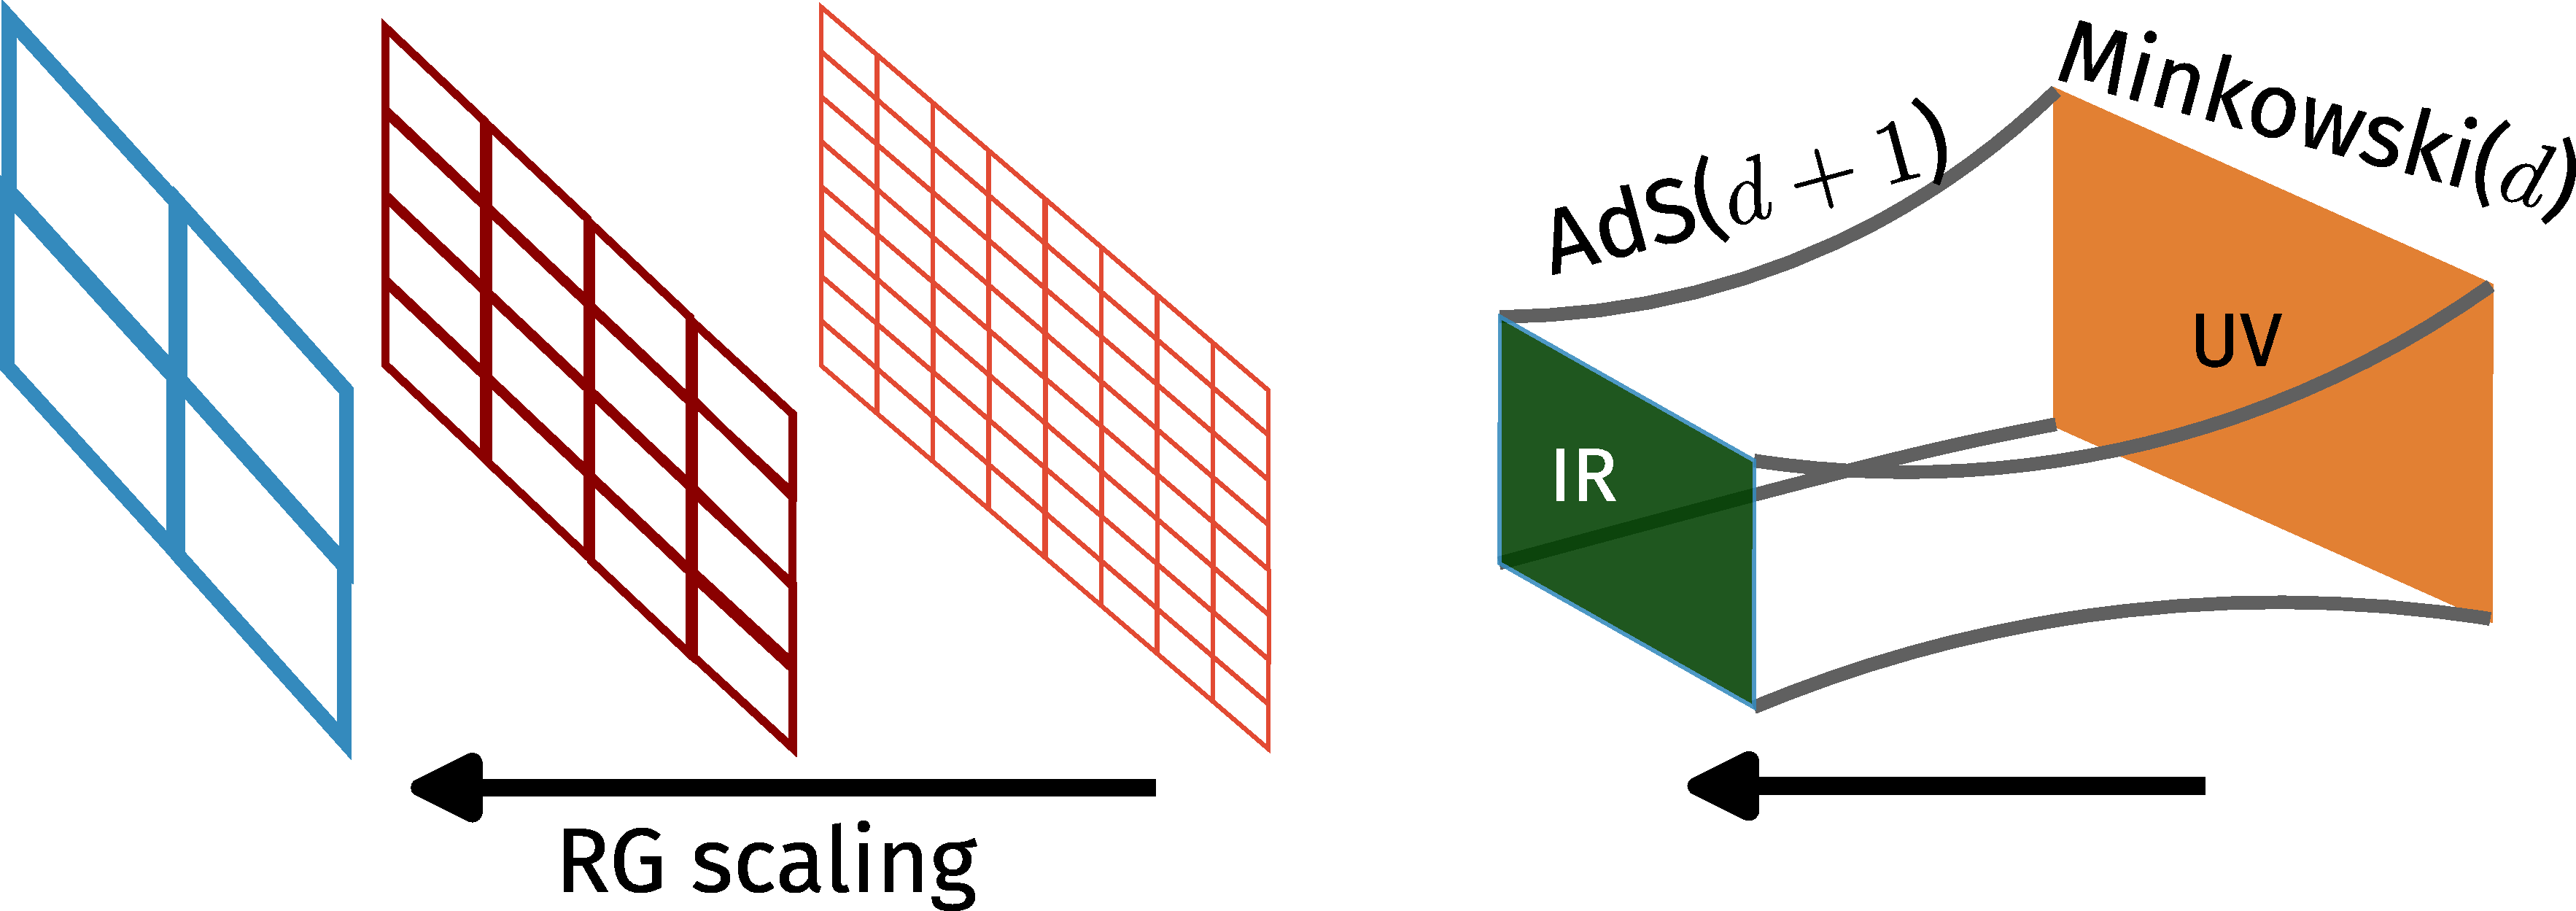
\includegraphics[width=\textwidth]{figures/holography.pdf}
\end{minipage}

\end{frame}

\begin{frame}{Creating subsystems}
	\[\text{Free Dirac fermions on torus:}~ ~ ~ k_x^n = \frac{2\pi }{L_x} n,~ ~ n \in \mathbb{Z};~~~ \text{define \alert{sparsity}} = \Delta n = 1\]
	\alert{Simplest} choice: the entire set
	\[\text{sparsity} = 1 \longrightarrow n \in \left\{-N,-(N-1),-(N-2),\ldots,-1,0,1,\ldots,N-2,N-1,N\right\} \]
	\alert{Coarser} choices: increase sparsity
	\[\text{sparsity} = 2 \longrightarrow n \in \left\{-N,-(N-2),-(N-4),\ldots,-2,0,2,\ldots,N-4,N-2,N\right\} \]
	\[\text{sparsity} = 4 \longrightarrow n \in \left\{-N,-(N-4),-(N-8),\ldots,-4,0,4,\ldots,N-8,N-4,N\right\} \]
	\centering
	\vspace*{\fill}
	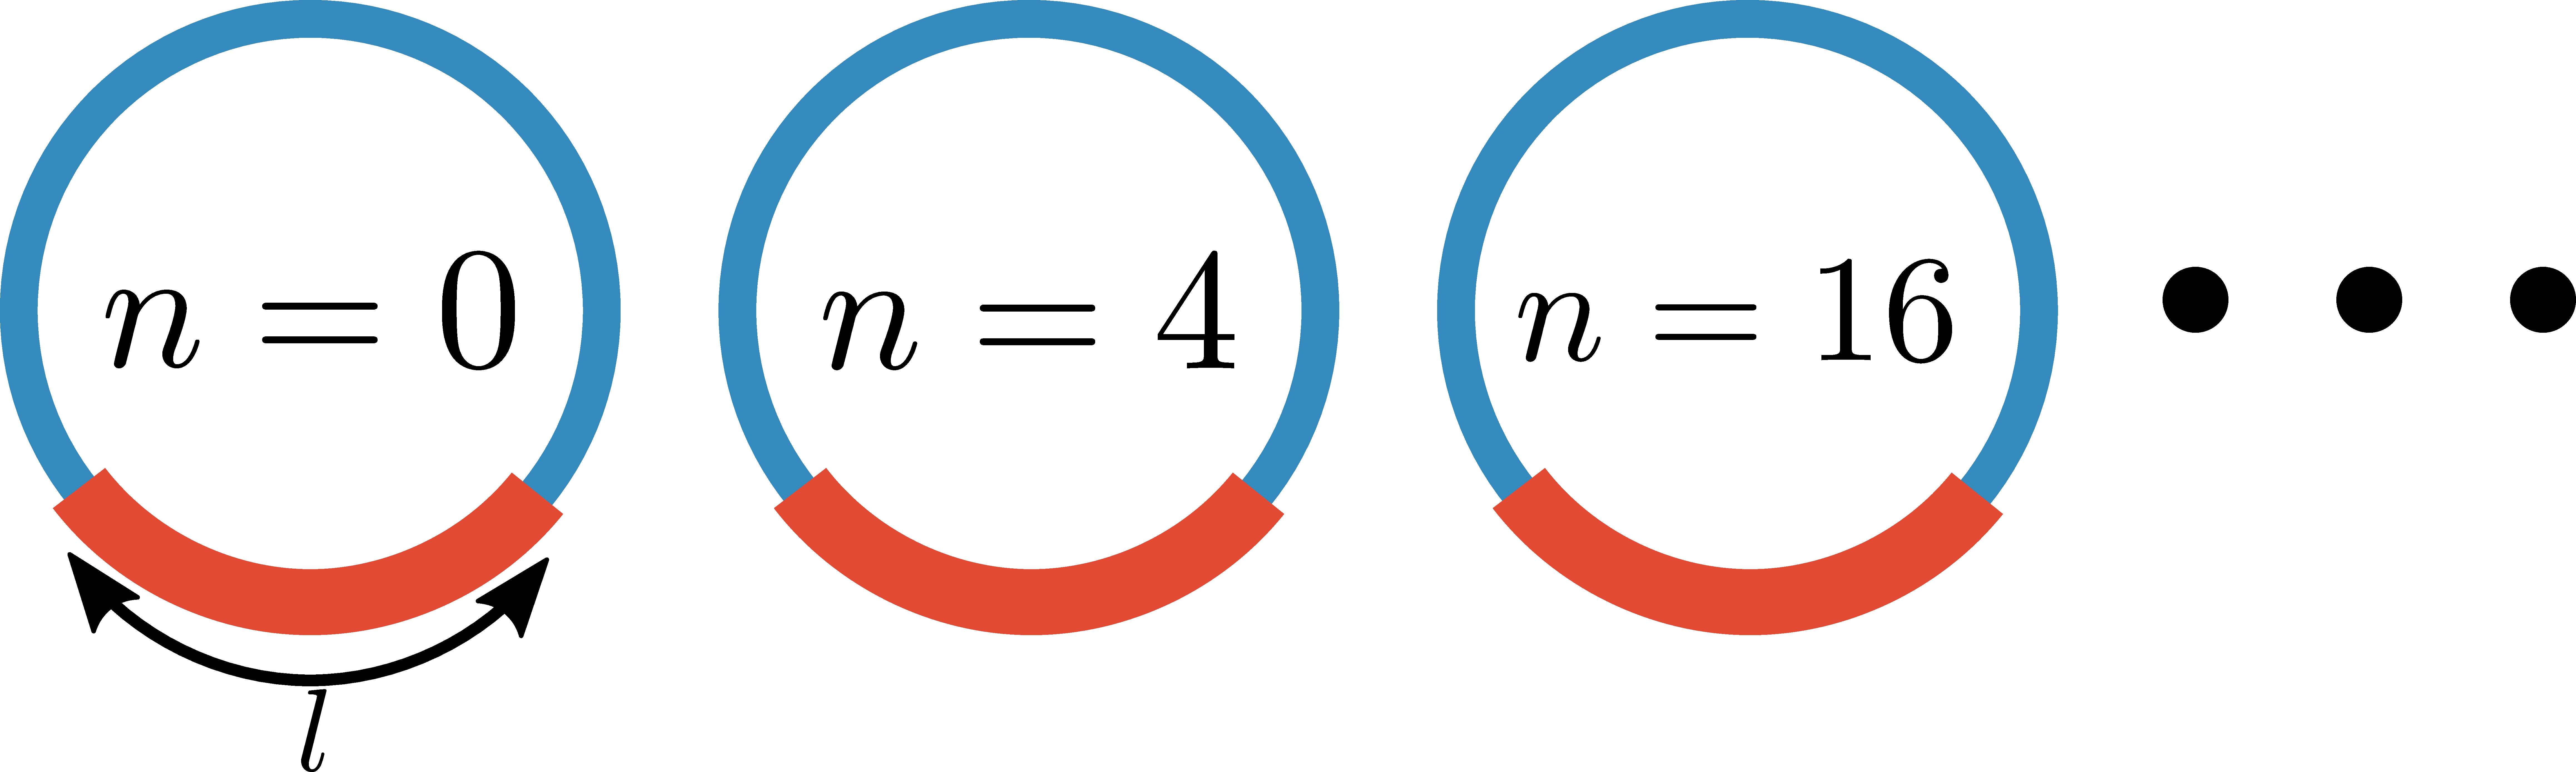
\includegraphics[width=0.4\textwidth]{figures/A_mi.pdf}
	\hspace*{\fill}
	\includegraphics[width=0.25\textwidth]{figures/subsystem-torus.pdf}
\end{frame}

\begin{frame}{Subsystem entanglement entropy: Entanglement hierarchy}
\footcite{Calabrese_2004,Casini_2005,Arias_2015,Chen_2017,Murciano_2020}
\begin{minipage}{0.5\textwidth}
\[S_{\mathcal{A}_z(j)} = f_z(j) c \alpha L_x - c \log \big|2\sin\left(\pi f_z(j)\phi\right)\big|\]
\[i < j, ~ ~ S_{i\cup j} =
	\begin{cases}
	S_{i}, ~ ~ z > 0\\
	S_{j}, ~ ~ z < 0
	\end{cases}
\]
\end{minipage}
\begin{minipage}{0.45\textwidth}
\includegraphics[height=0.3\textheight]{figures/Matroshka.png}
\includegraphics[height=0.3\textheight]{figures/nested.png}
\end{minipage}

\vspace*{\fill}

\begin{itemize}
	\nitem 
presents a \alert{hierarchy} of entanglement \(\longrightarrow\) EE distributed across RG steps\\
RG transformation \(\longrightarrow\) reveals entanglement

\vspace*{\fill}
\nitem distribution of entanglement also present in \alert{multipartite} entanglement
\end{itemize}

\end{frame}

\begin{frame}{Mutual information = distance}
\footcite{van2010building,lee2016,anirban_mott_2022,lee2010,lee2014,qi2013,lee2016,anirbanurg1,anirbanurg2,ryu2006,ryu2006aspects,nozaki2012}
\alert{Mutual information}: ~ \(I^2(A:B) \equiv S(A) + S(B) - S(A \cup B)\) ~ ~ ~ (non-negative)\\[10pt]

	\begin{minipage}{0.5\textwidth}
	Define distances using mut. info.
	\[x_z(j) = \log t_z(j),~ ~ ~y_z(j) = \log t_z(j \pm 1)\]
	\[v_z(j) \equiv \Delta y_z(j)/\Delta x_z(j), ~~ v^\prime = \Delta v_z(j)/\Delta x_z(j)\]
	\[\text{Curvature as well:} ~ ~ ~\kappa_{z}(j) = \frac{v^\prime_z(j)}{\left[1 + v_z(j)^2\right]^\frac{3}{2}}\]
	\end{minipage}
	\begin{minipage}{0.49\textwidth}
		\includegraphics[width=\textwidth]{curvature-pos.pdf}
	\end{minipage}
\end{frame}

\begin{frame}{RG evolution = emergent distance}
	\footcite{maldacena1999large,ryu2006aspects,holzhey_1994}
\begin{itemize}
	\nitem Distances and curvature can be related to an RG \alert{beta function}\\[10pt]
	\nitem Amounts to an \alert{explicit demonstration} of the holographic principle\\[10pt]
	\nitem Sign of curvature is \alert{topological}, can be written in terms of winding numbers\\[10pt]
\end{itemize}
	
\end{frame}

\begin{frame}{Topological nature of geometry-independent term}
	\footcite{luttinger1960ground,luttinger1960fermi,oshikawa2000topological,seki2017topological,anirbanurg1,Heath_2020}
	\[S_{\mathcal{A}_z(j)} = f_z(j) c \alpha L_x - \underbrace{c \log \big|2\sin\left(\pi f_z(j)\phi\right)\big|}_{=Q(\phi),\text{geometry-independent term}}\]
	\begin{itemize}
	\nitem \(Q(\phi)\) is periodic in the flux \(\phi\), ~ \(\phi=1\) transports a charge across Fermi surface\\[10pt]
	\nitem pole structure of \(\left(\sin \frac{\pi}{4} - |\sin\left(\pi f_z(j)\right)\phi|\right)^{-1}\) counts number of states \(\longrightarrow\) tracks Luttinger volume\\[10pt]
	\nitem Luttinger volume is topological, so is \(Q(\phi)\); \(Q(\phi)\) can be expressed in terms of winding numbers
	\end{itemize}
	
\end{frame}

\begin{frame}{}
\section{Holography and topology of entanglement scaling in free fermions}
\end{frame}


\begin{frame}{}
\section{Future Prospects}
\end{frame}

\begin{frame}{Improvements to the auxiliary model}
\begin{itemize}
	\nitem Better model can be obtained by using multiple impurities\\[20pt]
	\nitem Allows entangled liquid-like insulating phases\\[20pt]
	\nitem Might also provide \(k-\)space resolution 
	\begin{itemize}
		\nitem partial gapping of Fermi surface?
		\nitem pseudogap phases\\[20pt]
	\end{itemize}
	\nitem Introducing general impurity filling
	\begin{itemize}
		\nitem new phases?
		\nitem dominant pair fluctuations?
	\end{itemize}
\end{itemize}
\end{frame}

\begin{frame}{A novel auxiliary model approach}
\begin{itemize}
\only<1>{
	\nitem Using local impurity models to create bulk lattice models (Bloch's theorem)
		\[ H_\text{bulk} = \sum_i H_\text{local}(i), ~ ~\Psi_\text{bulk}(\vec k) \sim \sum_i e^{i \vec{k}\cdot\vec{r}_i}\Psi_\text{local}(i)\]
	\nitem Relates bulk correlation functions to those of the auxiliary model\\[20pt]
	\nitem phase transition in the extended AIM \(\longrightarrow\) phase transition inthe bulk model, \alert{metal-insulator transition} in Hubbard-Heisenberg model\\[20pt]
}
\only<2>{
	\nitem Should be useful for studying other models of strong-correlations
		\begin{itemize}
			\nitem periodic Anderson/Kondo models
			\nitem Heisenberg models\\[20pt]
		\end{itemize}
	\nitem Another potential application: topologically active systems:
		\begin{itemize}
			\nitem Fractional quantum hall systems\\[20pt]
		\end{itemize}
	\nitem Extend the formalism towards higher order Greens functions
		\begin{itemize}
			\nitem two-particle Greens functions, doublon-holon correlations
			\nitem can provide more info on the MIT
		\end{itemize}
}
\end{itemize}
\end{frame}

\begin{frame}{Heavy-fermion materials}
\begin{itemize}
	\nitem Materials with very high quasiparticle masses\\[20pt]
	\nitem Outstanding questions exist about the nature of phases and phase transitions
		\begin{itemize}
			\nitem microscopic justification of certain phases
			\nitem theory for the strange metal excitations
			\nitem microscopic justification for the origin of unconventional superconductivity\\[20pt]
		\end{itemize}
	\nitem the URG, MERG and auxiliary model methods should prove useful
\end{itemize}
\end{frame}

\end{document}
